\documentclass[letterpaper, 10pt]{report}

\usepackage[spanish]{babel}
\usepackage{fullpage}
\usepackage{graphicx}
\usepackage[utf8]{inputenc}
\usepackage{color}
\usepackage{gensymb}
\usepackage{listings}    
\usepackage{import}
\usepackage{pythonhighlight}
 %%%%%%%%%%%%%%%%%%%%%%%%%%%%%%%%%%%%%%%%%%%%%%%%%%%%%%%%%%%%%%%%%%%%%%%%%%%%%%%% 
%%% ~ Arduino Language - Arduino IDE Colors ~                                  %%%
%%%                                                                            %%%
%%% Kyle Rocha-Brownell | 10/2/2017 | No Licence                               %%%
%%% -------------------------------------------------------------------------- %%%
%%%                                                                            %%%
%%% Place this file in your working directory (next to the latex file you're   %%%
%%% working on).  To add it to your project, place:                            %%%
%%%     %%%%%%%%%%%%%%%%%%%%%%%%%%%%%%%%%%%%%%%%%%%%%%%%%%%%%%%%%%%%%%%%%%%%%%%%%%%%%%%% 
%%% ~ Arduino Language - Arduino IDE Colors ~                                  %%%
%%%                                                                            %%%
%%% Kyle Rocha-Brownell | 10/2/2017 | No Licence                               %%%
%%% -------------------------------------------------------------------------- %%%
%%%                                                                            %%%
%%% Place this file in your working directory (next to the latex file you're   %%%
%%% working on).  To add it to your project, place:                            %%%
%%%     %%%%%%%%%%%%%%%%%%%%%%%%%%%%%%%%%%%%%%%%%%%%%%%%%%%%%%%%%%%%%%%%%%%%%%%%%%%%%%%% 
%%% ~ Arduino Language - Arduino IDE Colors ~                                  %%%
%%%                                                                            %%%
%%% Kyle Rocha-Brownell | 10/2/2017 | No Licence                               %%%
%%% -------------------------------------------------------------------------- %%%
%%%                                                                            %%%
%%% Place this file in your working directory (next to the latex file you're   %%%
%%% working on).  To add it to your project, place:                            %%%
%%%    \input{arduinoLanguage.tex}                                             %%%
%%% somewhere before \begin{document} in your latex file.                      %%%
%%%                                                                            %%%
%%% In your document, place your arduino code between:                         %%%
%%%   \begin{lstlisting}[language=Arduino]                                     %%%
%%% and:                                                                       %%%
%%%   \end{lstlisting}                                                         %%%
%%%                                                                            %%%
%%% Or create your own style to add non-built-in functions and variables.      %%%
%%%                                                                            %%%
 %%%%%%%%%%%%%%%%%%%%%%%%%%%%%%%%%%%%%%%%%%%%%%%%%%%%%%%%%%%%%%%%%%%%%%%%%%%%%%%% 

\usepackage{color}
\usepackage{listings}    
\usepackage{courier}

%%% Define Custom IDE Colors %%%
\definecolor{arduinoGreen}    {rgb} {0.17, 0.43, 0.01}
\definecolor{arduinoGrey}     {rgb} {0.47, 0.47, 0.33}
\definecolor{arduinoOrange}   {rgb} {0.8 , 0.4 , 0   }
\definecolor{arduinoBlue}     {rgb} {0.01, 0.61, 0.98}
\definecolor{arduinoDarkBlue} {rgb} {0.0 , 0.2 , 0.5 }

%%% Define Arduino Language %%%
\lstdefinelanguage{Arduino}{
  language=C++, % begin with default C++ settings 
%
%
  %%% Keyword Color Group 1 %%%  (called KEYWORD3 by arduino)
  keywordstyle=\color{arduinoGreen},   
  deletekeywords={  % remove all arduino keywords that might be in c++
                break, case, override, final, continue, default, do, else, for, 
                if, return, goto, switch, throw, try, while, setup, loop, export, 
                not, or, and, xor, include, define, elif, else, error, if, ifdef, 
                ifndef, pragma, warning,
                HIGH, LOW, INPUT, INPUT_PULLUP, OUTPUT, DEC, BIN, HEX, OCT, PI, 
                HALF_PI, TWO_PI, LSBFIRST, MSBFIRST, CHANGE, FALLING, RISING, 
                DEFAULT, EXTERNAL, INTERNAL, INTERNAL1V1, INTERNAL2V56, LED_BUILTIN, 
                LED_BUILTIN_RX, LED_BUILTIN_TX, DIGITAL_MESSAGE, FIRMATA_STRING, 
                ANALOG_MESSAGE, REPORT_DIGITAL, REPORT_ANALOG, SET_PIN_MODE, 
                SYSTEM_RESET, SYSEX_START, auto, int8_t, int16_t, int32_t, int64_t, 
                uint8_t, uint16_t, uint32_t, uint64_t, char16_t, char32_t, operator, 
                enum, delete, bool, boolean, byte, char, const, false, float, double, 
                null, NULL, int, long, new, private, protected, public, short, 
                signed, static, volatile, String, void, true, unsigned, word, array, 
                sizeof, dynamic_cast, typedef, const_cast, struct, static_cast, union, 
                friend, extern, class, reinterpret_cast, register, explicit, inline, 
                _Bool, complex, _Complex, _Imaginary, atomic_bool, atomic_char, 
                atomic_schar, atomic_uchar, atomic_short, atomic_ushort, atomic_int, 
                atomic_uint, atomic_long, atomic_ulong, atomic_llong, atomic_ullong, 
                virtual, PROGMEM,
                Serial, Serial1, Serial2, Serial3, SerialUSB, Keyboard, Mouse,
                abs, acos, asin, atan, atan2, ceil, constrain, cos, degrees, exp, 
                floor, log, map, max, min, radians, random, randomSeed, round, sin, 
                sq, sqrt, tan, pow, bitRead, bitWrite, bitSet, bitClear, bit, 
                highByte, lowByte, analogReference, analogRead, 
                analogReadResolution, analogWrite, analogWriteResolution, 
                attachInterrupt, detachInterrupt, digitalPinToInterrupt, delay, 
                delayMicroseconds, digitalWrite, digitalRead, interrupts, millis, 
                micros, noInterrupts, noTone, pinMode, pulseIn, pulseInLong, shiftIn, 
                shiftOut, tone, yield, Stream, begin, end, peek, read, print, 
                println, available, availableForWrite, flush, setTimeout, find, 
                findUntil, parseInt, parseFloat, readBytes, readBytesUntil, readString, 
                readStringUntil, trim, toUpperCase, toLowerCase, charAt, compareTo, 
                concat, endsWith, startsWith, equals, equalsIgnoreCase, getBytes, 
                indexOf, lastIndexOf, length, replace, setCharAt, substring, 
                toCharArray, toInt, press, release, releaseAll, accept, click, move, 
                isPressed, isAlphaNumeric, isAlpha, isAscii, isWhitespace, isControl, 
                isDigit, isGraph, isLowerCase, isPrintable, isPunct, isSpace, 
                isUpperCase, isHexadecimalDigit, 
                }, 
  morekeywords={   % add arduino structures to group 1
                break, case, override, final, continue, default, do, else, for, 
                if, return, goto, switch, throw, try, while, setup, loop, export, 
                not, or, and, xor, include, define, elif, else, error, if, ifdef, 
                ifndef, pragma, warning,
                }, 
% 
%
  %%% Keyword Color Group 2 %%%  (called LITERAL1 by arduino)
  keywordstyle=[2]\color{arduinoBlue},   
  keywords=[2]{   % add variables and dataTypes as 2nd group  
                HIGH, LOW, INPUT, INPUT_PULLUP, OUTPUT, DEC, BIN, HEX, OCT, PI, 
                HALF_PI, TWO_PI, LSBFIRST, MSBFIRST, CHANGE, FALLING, RISING, 
                DEFAULT, EXTERNAL, INTERNAL, INTERNAL1V1, INTERNAL2V56, LED_BUILTIN, 
                LED_BUILTIN_RX, LED_BUILTIN_TX, DIGITAL_MESSAGE, FIRMATA_STRING, 
                ANALOG_MESSAGE, REPORT_DIGITAL, REPORT_ANALOG, SET_PIN_MODE, 
                SYSTEM_RESET, SYSEX_START, auto, int8_t, int16_t, int32_t, int64_t, 
                uint8_t, uint16_t, uint32_t, uint64_t, char16_t, char32_t, operator, 
                enum, delete, bool, boolean, byte, char, const, false, float, double, 
                null, NULL, int, long, new, private, protected, public, short, 
                signed, static, volatile, String, void, true, unsigned, word, array, 
                sizeof, dynamic_cast, typedef, const_cast, struct, static_cast, union, 
                friend, extern, class, reinterpret_cast, register, explicit, inline, 
                _Bool, complex, _Complex, _Imaginary, atomic_bool, atomic_char, 
                atomic_schar, atomic_uchar, atomic_short, atomic_ushort, atomic_int, 
                atomic_uint, atomic_long, atomic_ulong, atomic_llong, atomic_ullong, 
                virtual, PROGMEM,
                },  
% 
%
  %%% Keyword Color Group 3 %%%  (called KEYWORD1 by arduino)
  keywordstyle=[3]\bfseries\color{arduinoOrange},
  keywords=[3]{  % add built-in functions as a 3rd group
                Serial, Serial1, Serial2, Serial3, SerialUSB, Keyboard, Mouse,
                },      
%
%
  %%% Keyword Color Group 4 %%%  (called KEYWORD2 by arduino)
  keywordstyle=[4]\color{arduinoOrange},
  keywords=[4]{  % add more built-in functions as a 4th group
                abs, acos, asin, atan, atan2, ceil, constrain, cos, degrees, exp, 
                floor, log, map, max, min, radians, random, randomSeed, round, sin, 
                sq, sqrt, tan, pow, bitRead, bitWrite, bitSet, bitClear, bit, 
                highByte, lowByte, analogReference, analogRead, 
                analogReadResolution, analogWrite, analogWriteResolution, 
                attachInterrupt, detachInterrupt, digitalPinToInterrupt, delay, 
                delayMicroseconds, digitalWrite, digitalRead, interrupts, millis, 
                micros, noInterrupts, noTone, pinMode, pulseIn, pulseInLong, shiftIn, 
                shiftOut, tone, yield, Stream, begin, end, peek, read, print, 
                println, available, availableForWrite, flush, setTimeout, find, 
                findUntil, parseInt, parseFloat, readBytes, readBytesUntil, readString, 
                readStringUntil, trim, toUpperCase, toLowerCase, charAt, compareTo, 
                concat, endsWith, startsWith, equals, equalsIgnoreCase, getBytes, 
                indexOf, lastIndexOf, length, replace, setCharAt, substring, 
                toCharArray, toInt, press, release, releaseAll, accept, click, move, 
                isPressed, isAlphaNumeric, isAlpha, isAscii, isWhitespace, isControl, 
                isDigit, isGraph, isLowerCase, isPrintable, isPunct, isSpace, 
                isUpperCase, isHexadecimalDigit, 
                },      
%
%
  %%% Set Other Colors %%%
  stringstyle=\color{arduinoDarkBlue},    
  commentstyle=\color{arduinoGrey},    
%          
%   
  %%%% Line Numbering %%%%
   numbers=left,                    
  numbersep=5pt,                   
  numberstyle=\color{arduinoGrey},    
  %stepnumber=2,                      % show every 2 line numbers
%
%
  %%%% Code Box Style %%%%
  breaklines=true,                    % wordwrapping
  tabsize=2,         
  basicstyle=\ttfamily  
}                                             %%%
%%% somewhere before \begin{document} in your latex file.                      %%%
%%%                                                                            %%%
%%% In your document, place your arduino code between:                         %%%
%%%   \begin{lstlisting}[language=Arduino]                                     %%%
%%% and:                                                                       %%%
%%%   \end{lstlisting}                                                         %%%
%%%                                                                            %%%
%%% Or create your own style to add non-built-in functions and variables.      %%%
%%%                                                                            %%%
 %%%%%%%%%%%%%%%%%%%%%%%%%%%%%%%%%%%%%%%%%%%%%%%%%%%%%%%%%%%%%%%%%%%%%%%%%%%%%%%% 

\usepackage{color}
\usepackage{listings}    
\usepackage{courier}

%%% Define Custom IDE Colors %%%
\definecolor{arduinoGreen}    {rgb} {0.17, 0.43, 0.01}
\definecolor{arduinoGrey}     {rgb} {0.47, 0.47, 0.33}
\definecolor{arduinoOrange}   {rgb} {0.8 , 0.4 , 0   }
\definecolor{arduinoBlue}     {rgb} {0.01, 0.61, 0.98}
\definecolor{arduinoDarkBlue} {rgb} {0.0 , 0.2 , 0.5 }

%%% Define Arduino Language %%%
\lstdefinelanguage{Arduino}{
  language=C++, % begin with default C++ settings 
%
%
  %%% Keyword Color Group 1 %%%  (called KEYWORD3 by arduino)
  keywordstyle=\color{arduinoGreen},   
  deletekeywords={  % remove all arduino keywords that might be in c++
                break, case, override, final, continue, default, do, else, for, 
                if, return, goto, switch, throw, try, while, setup, loop, export, 
                not, or, and, xor, include, define, elif, else, error, if, ifdef, 
                ifndef, pragma, warning,
                HIGH, LOW, INPUT, INPUT_PULLUP, OUTPUT, DEC, BIN, HEX, OCT, PI, 
                HALF_PI, TWO_PI, LSBFIRST, MSBFIRST, CHANGE, FALLING, RISING, 
                DEFAULT, EXTERNAL, INTERNAL, INTERNAL1V1, INTERNAL2V56, LED_BUILTIN, 
                LED_BUILTIN_RX, LED_BUILTIN_TX, DIGITAL_MESSAGE, FIRMATA_STRING, 
                ANALOG_MESSAGE, REPORT_DIGITAL, REPORT_ANALOG, SET_PIN_MODE, 
                SYSTEM_RESET, SYSEX_START, auto, int8_t, int16_t, int32_t, int64_t, 
                uint8_t, uint16_t, uint32_t, uint64_t, char16_t, char32_t, operator, 
                enum, delete, bool, boolean, byte, char, const, false, float, double, 
                null, NULL, int, long, new, private, protected, public, short, 
                signed, static, volatile, String, void, true, unsigned, word, array, 
                sizeof, dynamic_cast, typedef, const_cast, struct, static_cast, union, 
                friend, extern, class, reinterpret_cast, register, explicit, inline, 
                _Bool, complex, _Complex, _Imaginary, atomic_bool, atomic_char, 
                atomic_schar, atomic_uchar, atomic_short, atomic_ushort, atomic_int, 
                atomic_uint, atomic_long, atomic_ulong, atomic_llong, atomic_ullong, 
                virtual, PROGMEM,
                Serial, Serial1, Serial2, Serial3, SerialUSB, Keyboard, Mouse,
                abs, acos, asin, atan, atan2, ceil, constrain, cos, degrees, exp, 
                floor, log, map, max, min, radians, random, randomSeed, round, sin, 
                sq, sqrt, tan, pow, bitRead, bitWrite, bitSet, bitClear, bit, 
                highByte, lowByte, analogReference, analogRead, 
                analogReadResolution, analogWrite, analogWriteResolution, 
                attachInterrupt, detachInterrupt, digitalPinToInterrupt, delay, 
                delayMicroseconds, digitalWrite, digitalRead, interrupts, millis, 
                micros, noInterrupts, noTone, pinMode, pulseIn, pulseInLong, shiftIn, 
                shiftOut, tone, yield, Stream, begin, end, peek, read, print, 
                println, available, availableForWrite, flush, setTimeout, find, 
                findUntil, parseInt, parseFloat, readBytes, readBytesUntil, readString, 
                readStringUntil, trim, toUpperCase, toLowerCase, charAt, compareTo, 
                concat, endsWith, startsWith, equals, equalsIgnoreCase, getBytes, 
                indexOf, lastIndexOf, length, replace, setCharAt, substring, 
                toCharArray, toInt, press, release, releaseAll, accept, click, move, 
                isPressed, isAlphaNumeric, isAlpha, isAscii, isWhitespace, isControl, 
                isDigit, isGraph, isLowerCase, isPrintable, isPunct, isSpace, 
                isUpperCase, isHexadecimalDigit, 
                }, 
  morekeywords={   % add arduino structures to group 1
                break, case, override, final, continue, default, do, else, for, 
                if, return, goto, switch, throw, try, while, setup, loop, export, 
                not, or, and, xor, include, define, elif, else, error, if, ifdef, 
                ifndef, pragma, warning,
                }, 
% 
%
  %%% Keyword Color Group 2 %%%  (called LITERAL1 by arduino)
  keywordstyle=[2]\color{arduinoBlue},   
  keywords=[2]{   % add variables and dataTypes as 2nd group  
                HIGH, LOW, INPUT, INPUT_PULLUP, OUTPUT, DEC, BIN, HEX, OCT, PI, 
                HALF_PI, TWO_PI, LSBFIRST, MSBFIRST, CHANGE, FALLING, RISING, 
                DEFAULT, EXTERNAL, INTERNAL, INTERNAL1V1, INTERNAL2V56, LED_BUILTIN, 
                LED_BUILTIN_RX, LED_BUILTIN_TX, DIGITAL_MESSAGE, FIRMATA_STRING, 
                ANALOG_MESSAGE, REPORT_DIGITAL, REPORT_ANALOG, SET_PIN_MODE, 
                SYSTEM_RESET, SYSEX_START, auto, int8_t, int16_t, int32_t, int64_t, 
                uint8_t, uint16_t, uint32_t, uint64_t, char16_t, char32_t, operator, 
                enum, delete, bool, boolean, byte, char, const, false, float, double, 
                null, NULL, int, long, new, private, protected, public, short, 
                signed, static, volatile, String, void, true, unsigned, word, array, 
                sizeof, dynamic_cast, typedef, const_cast, struct, static_cast, union, 
                friend, extern, class, reinterpret_cast, register, explicit, inline, 
                _Bool, complex, _Complex, _Imaginary, atomic_bool, atomic_char, 
                atomic_schar, atomic_uchar, atomic_short, atomic_ushort, atomic_int, 
                atomic_uint, atomic_long, atomic_ulong, atomic_llong, atomic_ullong, 
                virtual, PROGMEM,
                },  
% 
%
  %%% Keyword Color Group 3 %%%  (called KEYWORD1 by arduino)
  keywordstyle=[3]\bfseries\color{arduinoOrange},
  keywords=[3]{  % add built-in functions as a 3rd group
                Serial, Serial1, Serial2, Serial3, SerialUSB, Keyboard, Mouse,
                },      
%
%
  %%% Keyword Color Group 4 %%%  (called KEYWORD2 by arduino)
  keywordstyle=[4]\color{arduinoOrange},
  keywords=[4]{  % add more built-in functions as a 4th group
                abs, acos, asin, atan, atan2, ceil, constrain, cos, degrees, exp, 
                floor, log, map, max, min, radians, random, randomSeed, round, sin, 
                sq, sqrt, tan, pow, bitRead, bitWrite, bitSet, bitClear, bit, 
                highByte, lowByte, analogReference, analogRead, 
                analogReadResolution, analogWrite, analogWriteResolution, 
                attachInterrupt, detachInterrupt, digitalPinToInterrupt, delay, 
                delayMicroseconds, digitalWrite, digitalRead, interrupts, millis, 
                micros, noInterrupts, noTone, pinMode, pulseIn, pulseInLong, shiftIn, 
                shiftOut, tone, yield, Stream, begin, end, peek, read, print, 
                println, available, availableForWrite, flush, setTimeout, find, 
                findUntil, parseInt, parseFloat, readBytes, readBytesUntil, readString, 
                readStringUntil, trim, toUpperCase, toLowerCase, charAt, compareTo, 
                concat, endsWith, startsWith, equals, equalsIgnoreCase, getBytes, 
                indexOf, lastIndexOf, length, replace, setCharAt, substring, 
                toCharArray, toInt, press, release, releaseAll, accept, click, move, 
                isPressed, isAlphaNumeric, isAlpha, isAscii, isWhitespace, isControl, 
                isDigit, isGraph, isLowerCase, isPrintable, isPunct, isSpace, 
                isUpperCase, isHexadecimalDigit, 
                },      
%
%
  %%% Set Other Colors %%%
  stringstyle=\color{arduinoDarkBlue},    
  commentstyle=\color{arduinoGrey},    
%          
%   
  %%%% Line Numbering %%%%
   numbers=left,                    
  numbersep=5pt,                   
  numberstyle=\color{arduinoGrey},    
  %stepnumber=2,                      % show every 2 line numbers
%
%
  %%%% Code Box Style %%%%
  breaklines=true,                    % wordwrapping
  tabsize=2,         
  basicstyle=\ttfamily  
}                                             %%%
%%% somewhere before \begin{document} in your latex file.                      %%%
%%%                                                                            %%%
%%% In your document, place your arduino code between:                         %%%
%%%   \begin{lstlisting}[language=Arduino]                                     %%%
%%% and:                                                                       %%%
%%%   \end{lstlisting}                                                         %%%
%%%                                                                            %%%
%%% Or create your own style to add non-built-in functions and variables.      %%%
%%%                                                                            %%%
 %%%%%%%%%%%%%%%%%%%%%%%%%%%%%%%%%%%%%%%%%%%%%%%%%%%%%%%%%%%%%%%%%%%%%%%%%%%%%%%% 

\usepackage{color}
\usepackage{listings}    
\usepackage{courier}

%%% Define Custom IDE Colors %%%
\definecolor{arduinoGreen}    {rgb} {0.17, 0.43, 0.01}
\definecolor{arduinoGrey}     {rgb} {0.47, 0.47, 0.33}
\definecolor{arduinoOrange}   {rgb} {0.8 , 0.4 , 0   }
\definecolor{arduinoBlue}     {rgb} {0.01, 0.61, 0.98}
\definecolor{arduinoDarkBlue} {rgb} {0.0 , 0.2 , 0.5 }

%%% Define Arduino Language %%%
\lstdefinelanguage{Arduino}{
  language=C++, % begin with default C++ settings 
%
%
  %%% Keyword Color Group 1 %%%  (called KEYWORD3 by arduino)
  keywordstyle=\color{arduinoGreen},   
  deletekeywords={  % remove all arduino keywords that might be in c++
                break, case, override, final, continue, default, do, else, for, 
                if, return, goto, switch, throw, try, while, setup, loop, export, 
                not, or, and, xor, include, define, elif, else, error, if, ifdef, 
                ifndef, pragma, warning,
                HIGH, LOW, INPUT, INPUT_PULLUP, OUTPUT, DEC, BIN, HEX, OCT, PI, 
                HALF_PI, TWO_PI, LSBFIRST, MSBFIRST, CHANGE, FALLING, RISING, 
                DEFAULT, EXTERNAL, INTERNAL, INTERNAL1V1, INTERNAL2V56, LED_BUILTIN, 
                LED_BUILTIN_RX, LED_BUILTIN_TX, DIGITAL_MESSAGE, FIRMATA_STRING, 
                ANALOG_MESSAGE, REPORT_DIGITAL, REPORT_ANALOG, SET_PIN_MODE, 
                SYSTEM_RESET, SYSEX_START, auto, int8_t, int16_t, int32_t, int64_t, 
                uint8_t, uint16_t, uint32_t, uint64_t, char16_t, char32_t, operator, 
                enum, delete, bool, boolean, byte, char, const, false, float, double, 
                null, NULL, int, long, new, private, protected, public, short, 
                signed, static, volatile, String, void, true, unsigned, word, array, 
                sizeof, dynamic_cast, typedef, const_cast, struct, static_cast, union, 
                friend, extern, class, reinterpret_cast, register, explicit, inline, 
                _Bool, complex, _Complex, _Imaginary, atomic_bool, atomic_char, 
                atomic_schar, atomic_uchar, atomic_short, atomic_ushort, atomic_int, 
                atomic_uint, atomic_long, atomic_ulong, atomic_llong, atomic_ullong, 
                virtual, PROGMEM,
                Serial, Serial1, Serial2, Serial3, SerialUSB, Keyboard, Mouse,
                abs, acos, asin, atan, atan2, ceil, constrain, cos, degrees, exp, 
                floor, log, map, max, min, radians, random, randomSeed, round, sin, 
                sq, sqrt, tan, pow, bitRead, bitWrite, bitSet, bitClear, bit, 
                highByte, lowByte, analogReference, analogRead, 
                analogReadResolution, analogWrite, analogWriteResolution, 
                attachInterrupt, detachInterrupt, digitalPinToInterrupt, delay, 
                delayMicroseconds, digitalWrite, digitalRead, interrupts, millis, 
                micros, noInterrupts, noTone, pinMode, pulseIn, pulseInLong, shiftIn, 
                shiftOut, tone, yield, Stream, begin, end, peek, read, print, 
                println, available, availableForWrite, flush, setTimeout, find, 
                findUntil, parseInt, parseFloat, readBytes, readBytesUntil, readString, 
                readStringUntil, trim, toUpperCase, toLowerCase, charAt, compareTo, 
                concat, endsWith, startsWith, equals, equalsIgnoreCase, getBytes, 
                indexOf, lastIndexOf, length, replace, setCharAt, substring, 
                toCharArray, toInt, press, release, releaseAll, accept, click, move, 
                isPressed, isAlphaNumeric, isAlpha, isAscii, isWhitespace, isControl, 
                isDigit, isGraph, isLowerCase, isPrintable, isPunct, isSpace, 
                isUpperCase, isHexadecimalDigit, 
                }, 
  morekeywords={   % add arduino structures to group 1
                break, case, override, final, continue, default, do, else, for, 
                if, return, goto, switch, throw, try, while, setup, loop, export, 
                not, or, and, xor, include, define, elif, else, error, if, ifdef, 
                ifndef, pragma, warning,
                }, 
% 
%
  %%% Keyword Color Group 2 %%%  (called LITERAL1 by arduino)
  keywordstyle=[2]\color{arduinoBlue},   
  keywords=[2]{   % add variables and dataTypes as 2nd group  
                HIGH, LOW, INPUT, INPUT_PULLUP, OUTPUT, DEC, BIN, HEX, OCT, PI, 
                HALF_PI, TWO_PI, LSBFIRST, MSBFIRST, CHANGE, FALLING, RISING, 
                DEFAULT, EXTERNAL, INTERNAL, INTERNAL1V1, INTERNAL2V56, LED_BUILTIN, 
                LED_BUILTIN_RX, LED_BUILTIN_TX, DIGITAL_MESSAGE, FIRMATA_STRING, 
                ANALOG_MESSAGE, REPORT_DIGITAL, REPORT_ANALOG, SET_PIN_MODE, 
                SYSTEM_RESET, SYSEX_START, auto, int8_t, int16_t, int32_t, int64_t, 
                uint8_t, uint16_t, uint32_t, uint64_t, char16_t, char32_t, operator, 
                enum, delete, bool, boolean, byte, char, const, false, float, double, 
                null, NULL, int, long, new, private, protected, public, short, 
                signed, static, volatile, String, void, true, unsigned, word, array, 
                sizeof, dynamic_cast, typedef, const_cast, struct, static_cast, union, 
                friend, extern, class, reinterpret_cast, register, explicit, inline, 
                _Bool, complex, _Complex, _Imaginary, atomic_bool, atomic_char, 
                atomic_schar, atomic_uchar, atomic_short, atomic_ushort, atomic_int, 
                atomic_uint, atomic_long, atomic_ulong, atomic_llong, atomic_ullong, 
                virtual, PROGMEM,
                },  
% 
%
  %%% Keyword Color Group 3 %%%  (called KEYWORD1 by arduino)
  keywordstyle=[3]\bfseries\color{arduinoOrange},
  keywords=[3]{  % add built-in functions as a 3rd group
                Serial, Serial1, Serial2, Serial3, SerialUSB, Keyboard, Mouse,
                },      
%
%
  %%% Keyword Color Group 4 %%%  (called KEYWORD2 by arduino)
  keywordstyle=[4]\color{arduinoOrange},
  keywords=[4]{  % add more built-in functions as a 4th group
                abs, acos, asin, atan, atan2, ceil, constrain, cos, degrees, exp, 
                floor, log, map, max, min, radians, random, randomSeed, round, sin, 
                sq, sqrt, tan, pow, bitRead, bitWrite, bitSet, bitClear, bit, 
                highByte, lowByte, analogReference, analogRead, 
                analogReadResolution, analogWrite, analogWriteResolution, 
                attachInterrupt, detachInterrupt, digitalPinToInterrupt, delay, 
                delayMicroseconds, digitalWrite, digitalRead, interrupts, millis, 
                micros, noInterrupts, noTone, pinMode, pulseIn, pulseInLong, shiftIn, 
                shiftOut, tone, yield, Stream, begin, end, peek, read, print, 
                println, available, availableForWrite, flush, setTimeout, find, 
                findUntil, parseInt, parseFloat, readBytes, readBytesUntil, readString, 
                readStringUntil, trim, toUpperCase, toLowerCase, charAt, compareTo, 
                concat, endsWith, startsWith, equals, equalsIgnoreCase, getBytes, 
                indexOf, lastIndexOf, length, replace, setCharAt, substring, 
                toCharArray, toInt, press, release, releaseAll, accept, click, move, 
                isPressed, isAlphaNumeric, isAlpha, isAscii, isWhitespace, isControl, 
                isDigit, isGraph, isLowerCase, isPrintable, isPunct, isSpace, 
                isUpperCase, isHexadecimalDigit, 
                },      
%
%
  %%% Set Other Colors %%%
  stringstyle=\color{arduinoDarkBlue},    
  commentstyle=\color{arduinoGrey},    
%          
%   
  %%%% Line Numbering %%%%
   numbers=left,                    
  numbersep=5pt,                   
  numberstyle=\color{arduinoGrey},    
  %stepnumber=2,                      % show every 2 line numbers
%
%
  %%%% Code Box Style %%%%
  breaklines=true,                    % wordwrapping
  tabsize=2,         
  basicstyle=\ttfamily  
}

\lstdefinestyle{myArduino}{
  language=Arduino,
  %% Add other words needing highlighting below %%
  morekeywords=[1]{},                  % dark green
  morekeywords=[2]{FILE_WRITE},        % light blue
  morekeywords=[3]{SD, File},          % bold orange
  morekeywords=[4]{open, exists},      % orange
  %% The lines below add a nifty box around the code %%
  frame=shadowbox,                    
  rulesepcolor=\color{arduinoBlue},
}


\usepackage{lmodern}
\renewcommand*\familydefault{\sfdefault} %% Only if the base font of the document is to be sans serif
\usepackage[T1]{fontenc}

\title{\textbf{Curso de Capacitación}\\Arduino y Raspberry Pi Como Herramientas Didácticas\\ \textit{Apunte de Profundización}}
\author{Universidad Tecnológica de Chile -- INACAP\\
\textbf{Relator}: Antonio D. Vásquez Briones}
\date{\today}



\begin{document}
	\maketitle
	\tableofcontents
	
\begin{abstract}
	El presente documento, presenta diversos apuntes y material de apoyo para el curso \emph{Arduino y Raspberry Pi Como Herramientas Didácticas} orientado a académicos del \textbf{Área Informática y Telecomunicaciones}, dictado durante el mes de enero de 2018 en Sede Santiago Sur.
	
	Los tópicos tratados en este curso, están orientados a profesionales de las áreas mencionadas que no cuentan con conocimientos en estas plataformas, pero si cuentan con un trasfondo sólido de conocimientos en programación estructurada y sistemas operativos, como por ejemplo, el Lenguaje C y manejo básico de Sistemas Operativos basados en Linux.
	
	El apunte, está orientado para ser seguido junto con el avance del curso, el cual se estructura en tres capítulos que corresponden a las tres jornadas en que se dicta, de las cuales, se hace un esfuerzo para que cada una de estas, se subdivida en 4 bloques de dos horas, lo que corresponderían a las secciones de los capítulos correspondientes.
	
\end{abstract}
	
\chapter{Introducción}

\setlength{\parskip}{\baselineskip}
En este capítulo introductorio, se entrega información acerca de conceptos fundamentales involucrados en dos plataformas y proyectos \emph{Open-Source} independientes entre sí; {\bf Arduino} y {\bf Raspberry}. Estas plataformas, actualmente pasan por un evidente periodo de auge gracias a diversos portales en internet, al respaldo que han tenido por diversas instituciones educacionales de renombre alrededor del mundo y por sobre todo por contar con una gran y creciente comunidad que genera y comparte contenidos que permiten que muchas personas, con o sin tener una base de conocimientos en la materia, pueda poner en marcha interesantes proyectos de \emph{hágalo usted mismo} o \emph{Do It Yourself} DIY por sus siglas en inglés, por lo tanto, no es extraño que tanto  alumnos como docentes, constantemente insistan en la utilización de este tipo de plataformas, básicamente por que parece muy fácil y esta \emph{de moda}, cuando en realidad lo que se está haciendo es un \emph{copy-paste} desde internet, lo cual no es del todo algo malo. 

Por otro lado, el relator de esta capacitación, considera que la verdadera riqueza, está en que tenemos en nuestras manos, poderosas capacidades de cálculo que nos permitirán exprimir gran parte del conocimiento teórico que se imparte, en áreas ligadas a las Tecnologías de la Información y la Electrónica, puesto que en escencia estos artefactos, no son más que una implementación particular, de lo que desde décadas se ha venido enseñando, por lo tanto cualquier análisis desde la rigurosidad del \emph{Electrical Engineering and Computer Science} es posible y de hecho, resulta muy enriquecedor.

El llamado es, a no caer en que nuestros alumnos sean meros repetidores de proyectos que encuentran en la web, si no que estos puedan articular e integrar implementaciones, para crear más y mejores proyectos, gracias un análisis riguroso, sustentado en conocimientos sólidos en cada una de sus áreas.

\section{Microntroladores y Microprocesadores}
	
	Desde los años 90, por estos lados del mundo (Chile), con el auge de la computación y posteriormente internet, el término \textbf{Micro-Procesador}, nos resulta bastante familiar. A grandes rasgos, sabemos que se trata del \emph{cerebro} del sistema computacional, al punto que hoy en día se nos viene de inmediato a la cabeza exponentes como, \emph{Intel Core i7}, \emph{AMD Ryzen}, \emph{Intel Pentium}, \emph{AMD A9} por nombrar algunos. Por otro lado, existen por doquier, en nuestros dispositivos, como celulares, teclados, televisores, hornos micro-ondas, etc. otro tipo de dispositivos muy parecidos en arquitectura y funcionalidades; los \textbf{Micro-Controladores}, que están siempre silenciosamente, encargándose de tareas específicas, como por ejemplo, llevar el control de la potencia y el tiempo al calentar un plato en un Micro-ondas.
	
	\begin{figure}[h]
		\centering
		
\includegraphics[scale=0.8]{logoFabricantes.png}
		\caption{Principales Fabricantes actuales de Microprocesadores y Microcontroladores. \label{fabricantes}}
	\end{figure}
	
	Podemos entender inicialmente, estos dos tipos de dispositivos muy parecidos y diferentes a la vez, como bifurcaciones evolutivas de la máquina computacional. Así es, existe un mismo origen, por allá por 1971 en los albores de la compañía fabricante de \emph{chips} {\bf Intel}, se desarrolló el primer microprocesador {\bf Intel 4040}. El problema que resolvía era simple: Calcular, pues era parte de las calculadoras \emph{Busicom} de la época y más tarde el microprocesador {\bf Intel 8086} cómo parte de los primeros ordenadores, es decir, servían a los seres humanos en sus tareas con en el manejo y procesamiento de \emph{información} de manera rudimentaria, para ello, se valían de los principios de la electricidad y la electrónica para tomar \emph{información} del mundo real, procesarla a un nivel abstracto en forma de señales eléctricas y finalmente devolver el resultado final en forma de información inteligible por los seres humanos. Ese mismo potencial de cálculo desarrollado, podría ser utilizado para resolver problemas con señales eléctricas que actúan sobre elementos físicos en la industria y la vida cotidiana, para lo cual, no se requiere gran parte de los periféricos que trabajan con información \emph{humana}. En base a esta utilidad, nace el {\bf Microcontrolador} cómo un sistema computacional mínimo, pero completo inserto en un sólo chip, orientado principalmente a trabajar con señales eléctricas por sobre el manejo de información. \cite{libroMicro}
	
	Cabe notar, que en la actualidad la diferencia entre microprocesador y microcontrolador ha dejado de ser una línea bien definida, puesto que existen sistemas como los llamados \emph{System On Chip} SoC que utilizan microprocesadores conocidos insertos en un mismo chip junto a otros periféricos de un sistema computacional, sin ser un microcontrolador, y los \emph{Circuitos Integrados de Aplicación Específica} ASIC's que podrían integrar tanto microprocesadores o microcontroladores en su diseño sin que sea necesario que su fabricante especifique su diseño interno. Toda esta gama de dispositivos y aplicaciones conforman el área de especialización llama \textbf{Sistemas Embebidos} o Embedded Systems. 
	
\section{Placa de Desarrollo Arduino UNO}
	\begin{figure}[h]
		\centering
		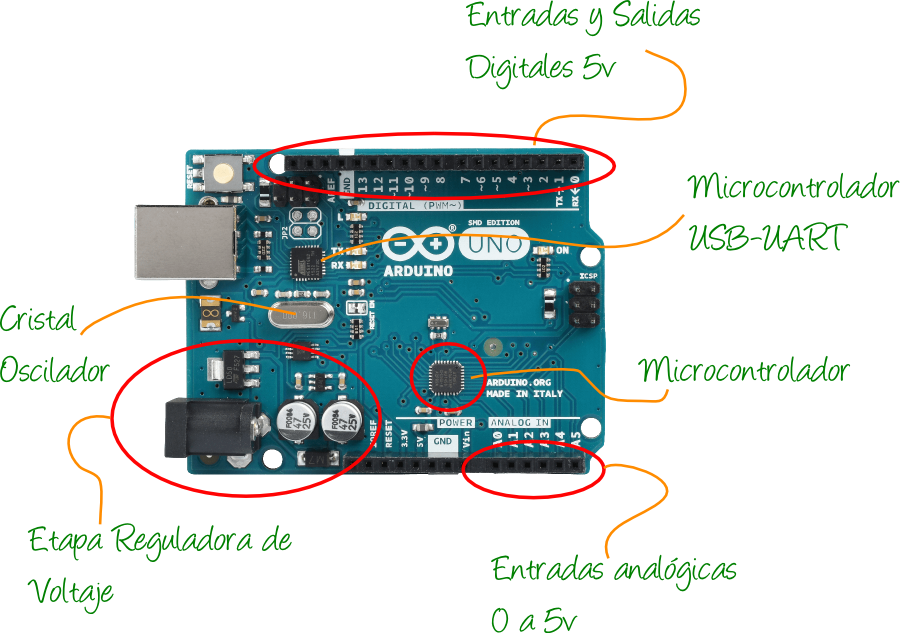
\includegraphics[scale=0.6]{anatomiaArduino.png}
		\caption{Anatomía de la Tarjeta de Desarrollo Arduino Uno. \label{anatomiaArduino}}	
	\end{figure}			
		
		Arduino Uno, es una \textbf{Tarjeta de Desarrollo} basada en el Microcontrolador de Atmel ATmega328p, precargada con un \emph{Bootloader} que permite la programación del microcontrolador directamente desde un puerto serial UART. Contiene los periféricos asociados que permiten que el microcontrolador entre en funcionamiento, tal cómo se puede apreciar en la imagen \ref{anatomiaArduino}, donde tenemos:
		
		
		\begin{itemize}

			\item {\bf Cristal Oscilador:} Encargado de entregar la  \emph{señal de reloj} para que el microcontrolador pueda ejecutar instrucción tras instrucción. Funciona en base al \textbf{Efecto Piezoeléctrico}.
			\item {\bf Etapa de alimentación:} Regula el voltaje aplicado como alimentación a ambos microcontroladores--principal y de comunicación-- puede  recibir de forma segura voltajes de entrada hasta los 12 volts y entregar un voltaje estable de 5 volts.
		  
			\item {\bf Comunicación USB-Serial UART:} Es un microcontrolador adicional, incluido en las últimas versiones de arduino\footnote{Desde la versión R3 en adelante. La mayoria de las placas \emph{arduino compatible}, no tienen este chip y traen el dispositivo CH340g, el cual no es programable y solo se encarga de la comunicación SERIAL-USB a UART-TTL}, está programado para emular comunicación serial sobre usb, lo que permite programar el chip principal y establecer comunicación entre el PC y Arduino. También es programable (DFU programming) y permite generar dispositivos usb nativos \emph{Human Inteface Device} HID como teclados, mouse, controladores midi, entre otros.
			
			\item \textbf{Pines de entradas y salidas digitales: } Son conexiones eléctricas directas con pines específicos del microcontrolador y son las encargadas de convertir señales eléctricas en bits o vice-versa al interior de un programa. Funcionan detectando o emitiendo voltajes de 0 ó 5 volts, los cuales serán interpretados a nivel de programa como estados \texttt{HIGH} o \texttt{LOW}. Habitualmente el umbral de detección se encuentra alrededor de los 3 volts, es decir, todo voltaje aplicado a un pin digital, entre 3 y 5.5 volts será considerado como estado \texttt{HIGH} y si esta entre 3 volts y 0 volts, será un estado \texttt{LOW}. \cite{atmegaDatasheet}
			
			\item {\bf Pines de Entradas Analógicas:} Permiten que el sistema lea en forma de voltaje, información proveniente de variables continuas por medio de diversos tipos de sensores. 
		\end{itemize}
		
\section{Single Board Computer Raspberry Pi}

	Raspberry Pi, es básicamente un computador tal y como los conocemos, muy pequeño, del tamaño de una tarjeta de crédito, pero bastante reducido en recursos. Podríamos decir, que se asemeja en desempeño a un computador de hace unos ocho a diez años atrás, aunque evidentemente tiene más y mejor tecnología que aquellos de antaño y lo mejor, a un muy bajo costo.
	
\begin{figure}[h]
		\centering
		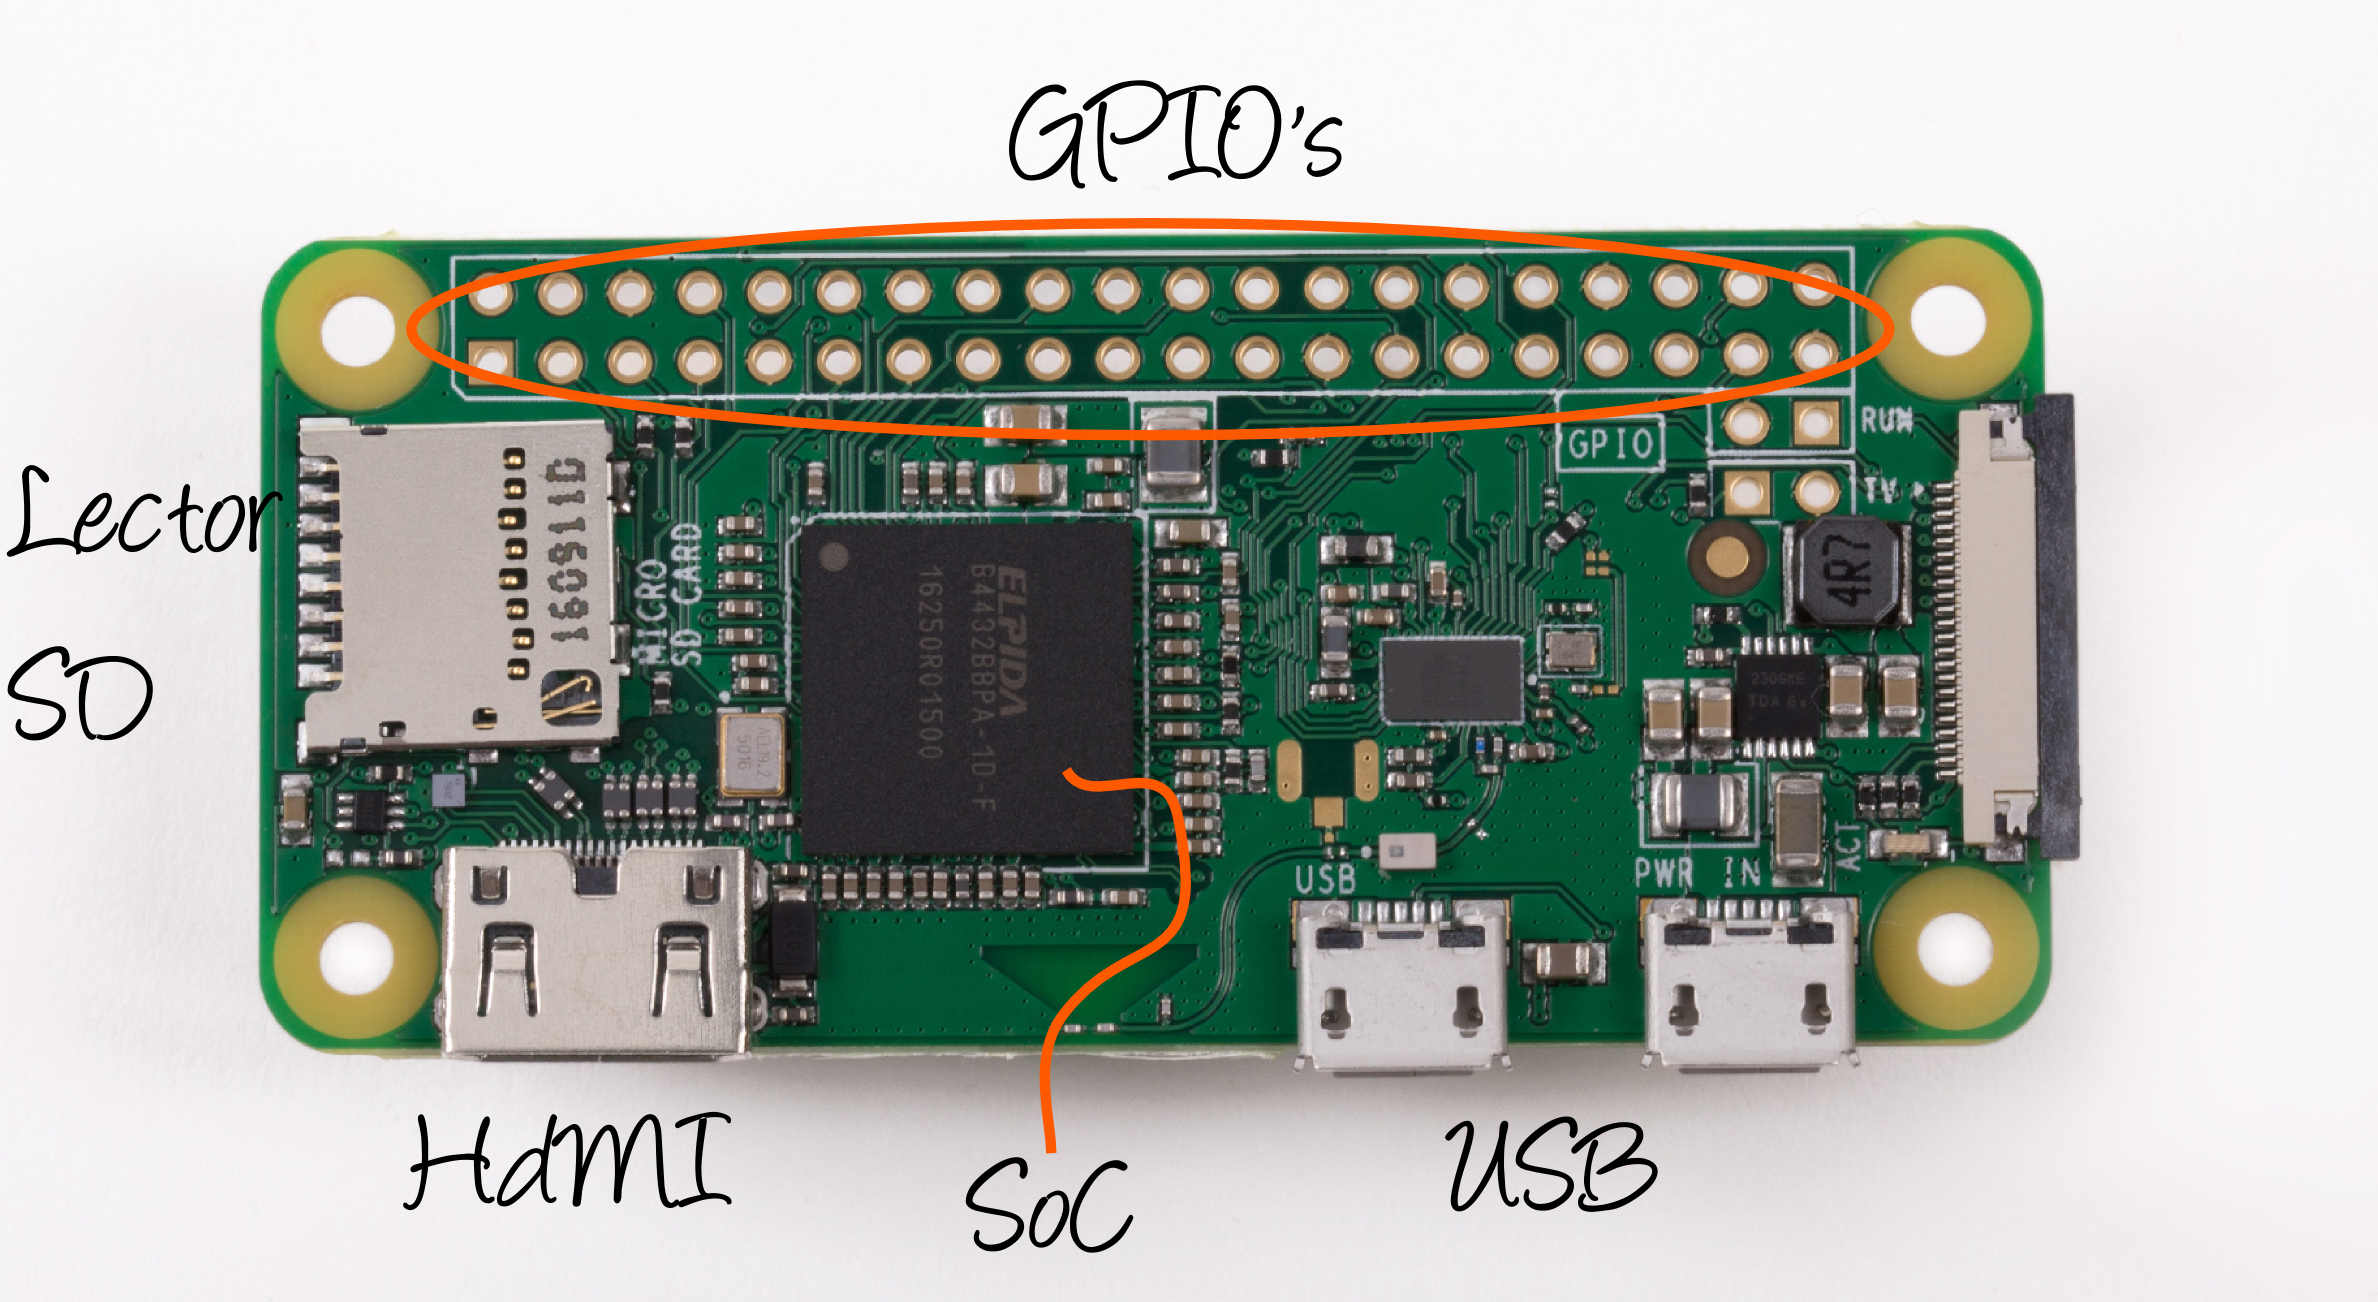
\includegraphics[scale=0.2]{anatomiaRaspberry.png}
		\caption{Raspberry Pi Zero (6.5 cm de longitud)\label{anatomiaRaspberry}}
\end{figure}
	
	En términos de hardware, se trata de un sistema con arquitectura ARM--como los smartphone--integrado con memoria ram y capacidades de video en un mismo chip\footnote{Aunque esto cae en la definición de microcontrolador, la complejidad del procesador califica a todo el sistema dentro de la categoría SoC} acompañado con periféricos como un Bus USB, un lector de tarjetas SD, interfaz de red y una interfaz física de video cómo HDMI o salida analógica de video, adicionalmente, posee interfaces especificas que los computadores utilizan para manejar circuitería interna en redes de bajo nivel, como buses SPI, I2C, los clásicos UART para comunicación Serial y unos pines de entrada o salidas que serían algo así como bits físicos, llamados GPIO, {\it General Purpose Input Output}. Todas las variantes de raspberry, corresponden a la misma arquitectura, por ejemplo en la figura \ref{anatomiaRaspberry}, se puede ver el caso de la más pequeña de todas, Raspberry Pi Zero.
	
	En términos de conocimientos necesarios para dominar sistemas con Raspberry Pi, cabe notar que se trata de un computador, por lo tanto, el conocimiento requerido depende más del sistema operativo que del dominio del hardware. Por excelencia, desde su creación ha sido la variante de Debian, \textbf{Raspbian}, que contiene precargados numerosos software que permiten probar funcionalidades básicas, pero no se debe olvidar que su potencial es el mismo que cualquier sistema Linux, por ende puede ser programado en diversos lenguajes, al igual que cualquier sistema operativo. Adicionalmente existen muchas \emph{distros}\footnote{Personalizaciones de linux como Ubuntu, Debian, Linux Mint, Fedora, entre otras} linux, especificas para Raspberry e incluso existe Windows CE, un sistema ampliamente utilizado por computadores embebidos a nivel industrial.	
	
	\chapter{Ecosistema Arduino y Control Digital}
	
	\section{?`Qué es Arduino?}
	
	\begin{center}
		
\includegraphics[scale=0.3]{awpLogo.png}
	\end{center}

	Arduino es una plataforma de \textbf{Electrónica de Código Abierto}--\emph{Open Source Electronics Platform}-- basada en hardware y software que se caracterizan por su facilidad de uso. Las tarjetas de desarrollo Arduino pueden leer entradas desde el mundo físico real, realizar un procesamiento a nivel de datos y devolver algún tipo de interacción con el mundo real, en forma de Luz, Movimiento, Sonido, etc. Para usar un arduino, se hace programándola directamente desde un computador por medio del \emph{Lenguaje Arduino}\footnote{Es una API implementada en lenguaje C++ con instrucciones intuitivas que permiten realizar tareas simples.} heredado de un proyecto anterior llamado \emph{Wiring}, el Entorno Integrado de Desarrollo (IDE por sus siglas en inglés) está basado también en un proyecto similar llamado \emph{Processing}.\footnote{Una API implementada en Java para programar contenido audiovisual.}

A lo largo de los años, Arduino ha sido el \emph{Cerebro} de miles de proyectos, desde objetos cotidianos hasta instrumentos y aplicaciones científicas. Gran parte del éxito de esta plataforma, se debe a una gran comunidad alrededor del mundo de \emph{Makers}, estudiantes, entusiastas, artistas, programadores y profesionales que han permitido que este proyecto \emph{open-source} siga avanzando gracias a la contribucion de increibles cantidades de conocimiento accesible a través de la web que es de gran ayuda tanto para principiantes como expertos en el área.
 
%Over the years Arduino has been the brain of thousands of projects, from everyday objects to complex scientific instruments. A worldwide community of makers - students, hobbyists, artists, programmers, and professionals - has gathered around this open-source platform, their contributions have added up to an incredible amount of accessible knowledge that can be of great help to novices and experts alike.

Arduino nace en el \emph{Ivrea Interaction Design Institute} como una herramienta de fabricación rápida de prototipos, que permitiría que estudiantes sin un respaldo de conocimientos en electrónica y programación pudieran desarrollar proyectos tecnológicos. Tan rapidamente como se lograron alcanzar grandes comunidades el proyecto en si mismo comenzo a adaptarse a diversas necesidades de distintas áreas, al punto que hoy en día existe un amplio ecosistema tanto hardware como software que permite desarrollar desde simples aplicaciones hasta resolver desafíos actuales de la industria 4.0 como el control de procesos, internet de las Cosas, Domótica, impresión 3d, maquinas CNC, entre otras áreas. \cite{queEsArduino}. En la imagen \ref{awp} se puede apreciar el software Processing, la Placa Wiring S, y la primera versión de Arduino \emph{Duemilanove}.

\begin{figure}[h]
	\centering
	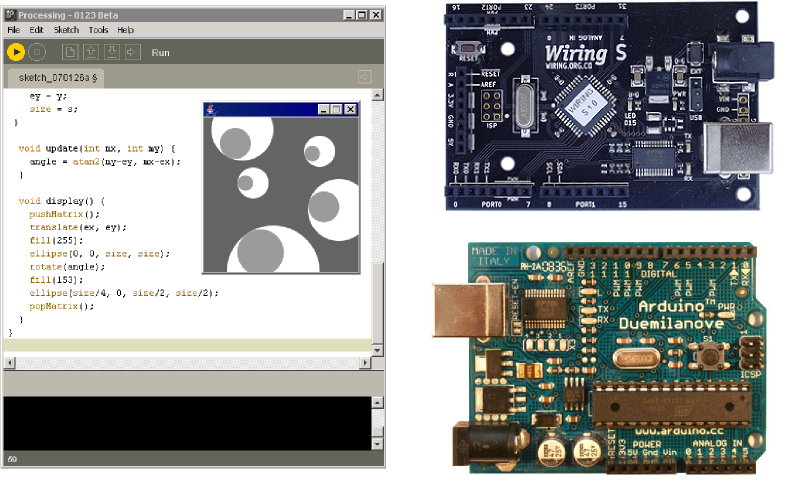
\includegraphics[scale=0.6]{awp.png}
	\caption{IDE processing, Placa Wiring S y Arduino Duemilanove. \label{awp}}
\end{figure}
	
\section{Primeros Pasos}

\subsection{Obtención del Entorno Integrado de Desarrollo}

El primer paso, para comenzar con Arduino, es descargar el Entorno Integrado de Desarrollo del mismo nombre, para ello es necesario un computador con acceso a internet. Habitualmente, es posible descargarlo desde el sigueiente sitio.

\begin{figure}[h]
	\centering
	\texttt{https://www.arduino.cc/en/main/software}\\
	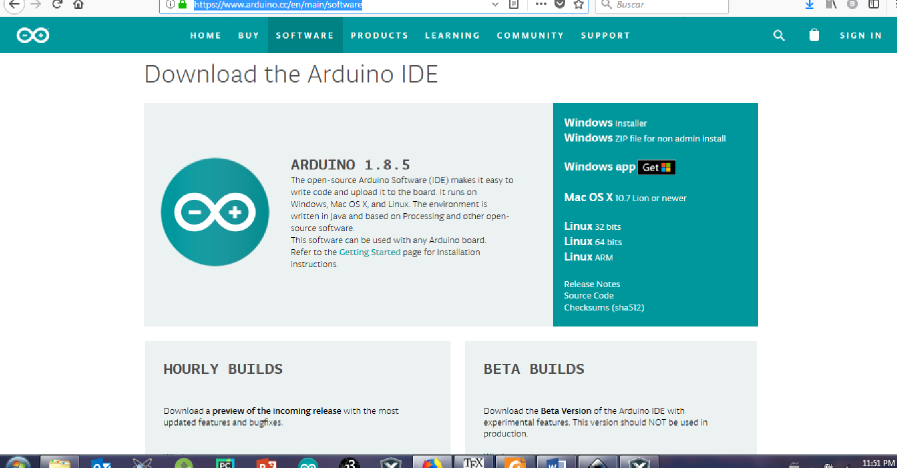
\includegraphics[scale=0.6]{download.png}
	\caption{Sitio de descarga del IDE Arduino.\label{descarga}}
\end{figure}		
		
En la imagen \ref{descarga}, se puede apreciar que existen dos instaladores de Windows, el primero es una instalación típica como cualquier software, mientras que el segundo \emph{Non-admin Installer} sirve para utilizar el software en maquinas que no tengan habilitados los permisos de administrador, lo cual, resulta de gran utilidad, pues es el caso de la mayoría de los PC's institucionales.

La instalación, como ha de esperarse en Windows, es presionar el boton siguiente hasta finalizar, con ello se instalan los drivers y todo lo necesario para que el sistema funcione. En sistemas Linux como Debian basta la instrucción \texttt{[sudo apt-get install arduino]} para instalar el software, puesto que se encuentra incluido en los repositorios oficiales. 
	
\subsection{Conexión de Arduino al PC y Configuración del IDE}

El siguiente paso, es conectar el Arduino al PC por medio del cable USB A-B o USB tipo D a un puerto cualquiera de nuestro computador, cabe notar que este puerto brindará energía para la mayoría de las experiencias que realizaremos. Una vez conectada, lo normal es que parpadeen algunos led's de la placa, dependiendo del programa que haya estado previamente cargado en cada una de las placas, puede que no se comporten todas igual.

Una de las maneras de asegurarnos de que toda la conexión está bien y que no hay problema de drivers en windows, es revisar el administrador de dispositivos (win+R devmgmt.msc) y buscar entre los dispositivos \emph{Puertos COM \& LPT} debería estar nuestra arduino en algún puerto COM cualquiera, tal como se muestra en la imagen \ref{debmgr}

\begin{figure}[h]
\centering
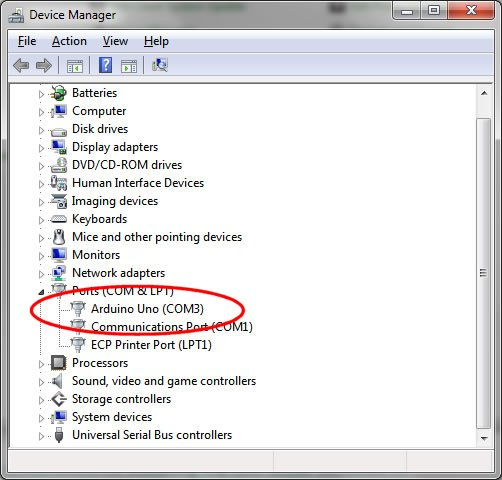
\includegraphics[scale=0.4]{device_manager.jpg}
\caption{Arduino Uno en Administrador de Dispositivos de Windows. \label{debmgr}}
\end{figure} 


Luego al abrir el IDE Arduino, podemos identificar los elementos mostrados en la figura \ref{ideArduino} y en la barra de menús superior, se debe escoger el modelo de placa con que estemos trabajando y el puerto COM al que stá conectada. (figura \ref{puertoplaca})
\begin{figure}
\centering
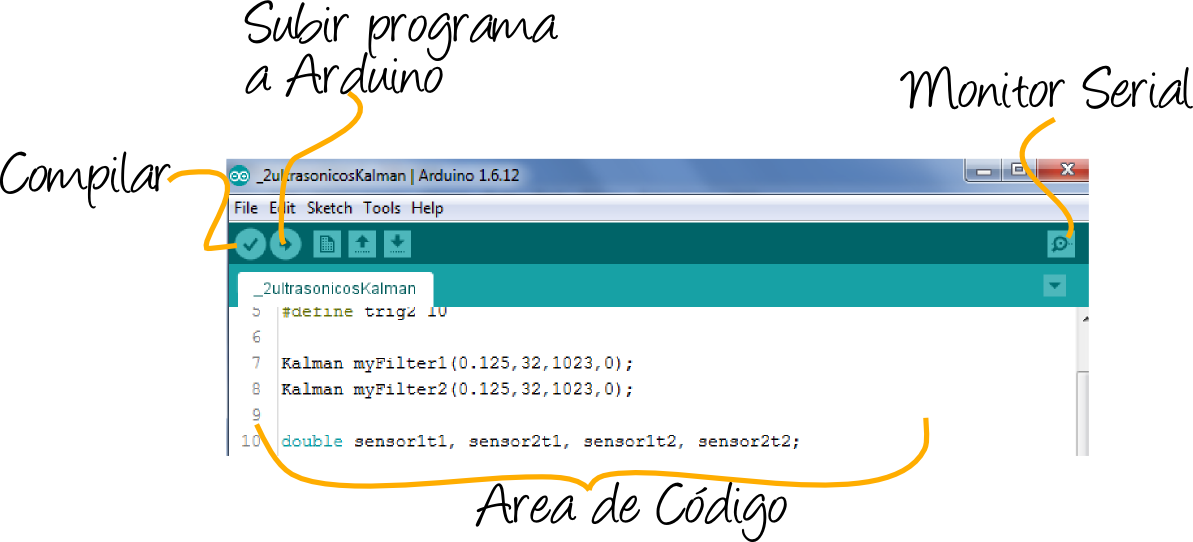
\includegraphics[scale=0.5]{ideArduino.png}
\caption{Elementos principales del IDE Arduino. \label{ideArduino}}
\end{figure}

\begin{figure}
\centering
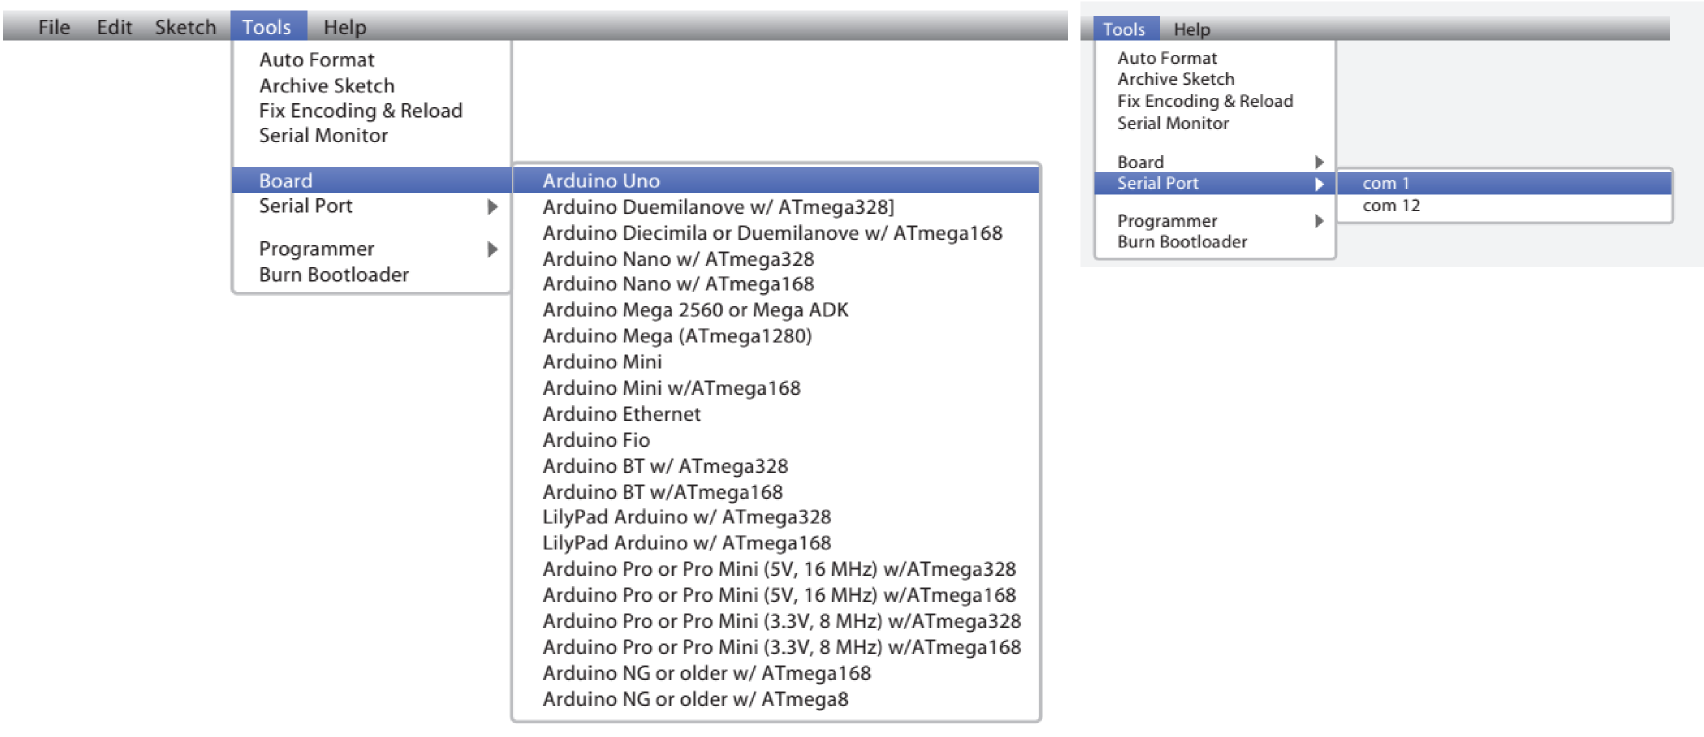
\includegraphics[scale=0.4]{puertoplaca.png}
\caption{Configuración de Modelo de Placa y Puerto COM. \label{puertoplaca}}
\end{figure}

Una vez realizado esto, podemos comenzar a programar nuestra Arduino.

\subsection{Estructura de un Código Arduino}

Como ya se mencionó antes, el Lenguaje Arduino, no es más que una API desarrollada en C++, por lo tanto, los fundamentos de programación estructurada en dicho lenguaje, se mantienen, por ejemplo, declaración de librerías, directivas al compilador, declaración de variables e incluso la mayoría de los tipos de variables en C se mantienen, de hecho Arduino utiliza un compilador cruzado GCC para arquitecturas Avr de Atmel.

La principal diferencia radica en un nuevo tipo de estructura en el código, que se separa en dos funciones principales de tipo \texttt{void} que son las siguientes:
\begin{itemize}
	\item \texttt{setup()}\\Función que se ejecuta una sola vez al encendido del microcontrolador, aquí se deben configurar entradas, salidas, periféricos y todo aquello que se desee realizar una sola vez para todo el tiempo de funcionamiento del sistema.
	
	\item \texttt{loop()}\\Bucle infinito que realizará repetidamente las instrucciones que se escriban dentro de el, originalmente está implementado con un \texttt{while(1)}. Aquí se realizan las operaciones principales del microcontrolador, como lectura de sensores, envío de datos y todo aquello que se quiera que esté realizando constantemente el microcontrolador.
\end{itemize}

\section{Control de Salidas Digitales}

A continuación, se muestra un código que sería el equivalente a un \emph{Hola Mundo} en computación física. Este se puede encontrar dentro de la gran colección de ejemplos que trae el software. (\texttt{File>Examples>Basics>Blink})
\\
\begin{lstlisting}[style=myArduino]
void setup() {  
  pinMode(13, OUTPUT);
}

void loop() {
  digitalWrite(13, HIGH);   // turn the LED on (HIGH is the voltage level)
  delay(1000);              // wait for a second
  digitalWrite(13, LOW);    // turn the LED off by making the voltage LOW
  delay(1000);              // wait for a second
}
\end{lstlisting}

Este código, pone a parpadear un Led integrado en la placa arduino, el cual está internamente conectado al Pin 13 de la tarjeta.

De aquí podemos analizar las instrucciones utilizadas:
\begin{itemize}
\item \texttt{pinMode(13,OUTPUT)}\\
Declara el pin número 13 del arduino como salida. Si cambiamos el número 13 por otro entre 0 y 12, la declaración afectará al pin correspondiente. De la misma manera, si se quiere que el pin sea entrada, basta cambiar \texttt{OUTPUT} por \texttt{INPUT}.

\item \texttt{digitalWrite(13,LOW)}\\
Como su nombre lo dice, realiza la escritura digital de un estado \texttt{LOW} en el pin 13. Cambiar el número afectará a otro pin, y para estados altos usamos la palaba \texttt{HIGH}.

\item \texttt{delay(1000)}\\
Genera un retardo de 1000 \textbf{mili-segundos} despues de la instrucción anterior. Si cambiamos ese número, esa será la cantidad de milisegundos que el microcontrolador quedará \emph{paralizado}. Cabe notar que el micro no puede ejecutar ninguna otra tarea durante el delay. Para retardos del orden de micro-segundos se utiliza la instrucción \texttt{delayMicroseconds(retardo)}.
\end{itemize}

\subsection{Actividad}
\begin{enumerate}
\item Cargue el programa en inicial en el microcontrolador y verifique su funcionamiento físico.
\item Juegue con valores extremadamente pequeños para el delay y comente acerca del efecto visual que se produce.
\item Realice el montaje del circuito mostrado en la figura \ref{circ}.
\item Modifique su código para hacer funcionar el circuito montado.
\end{enumerate}

\begin{figure}
\centering
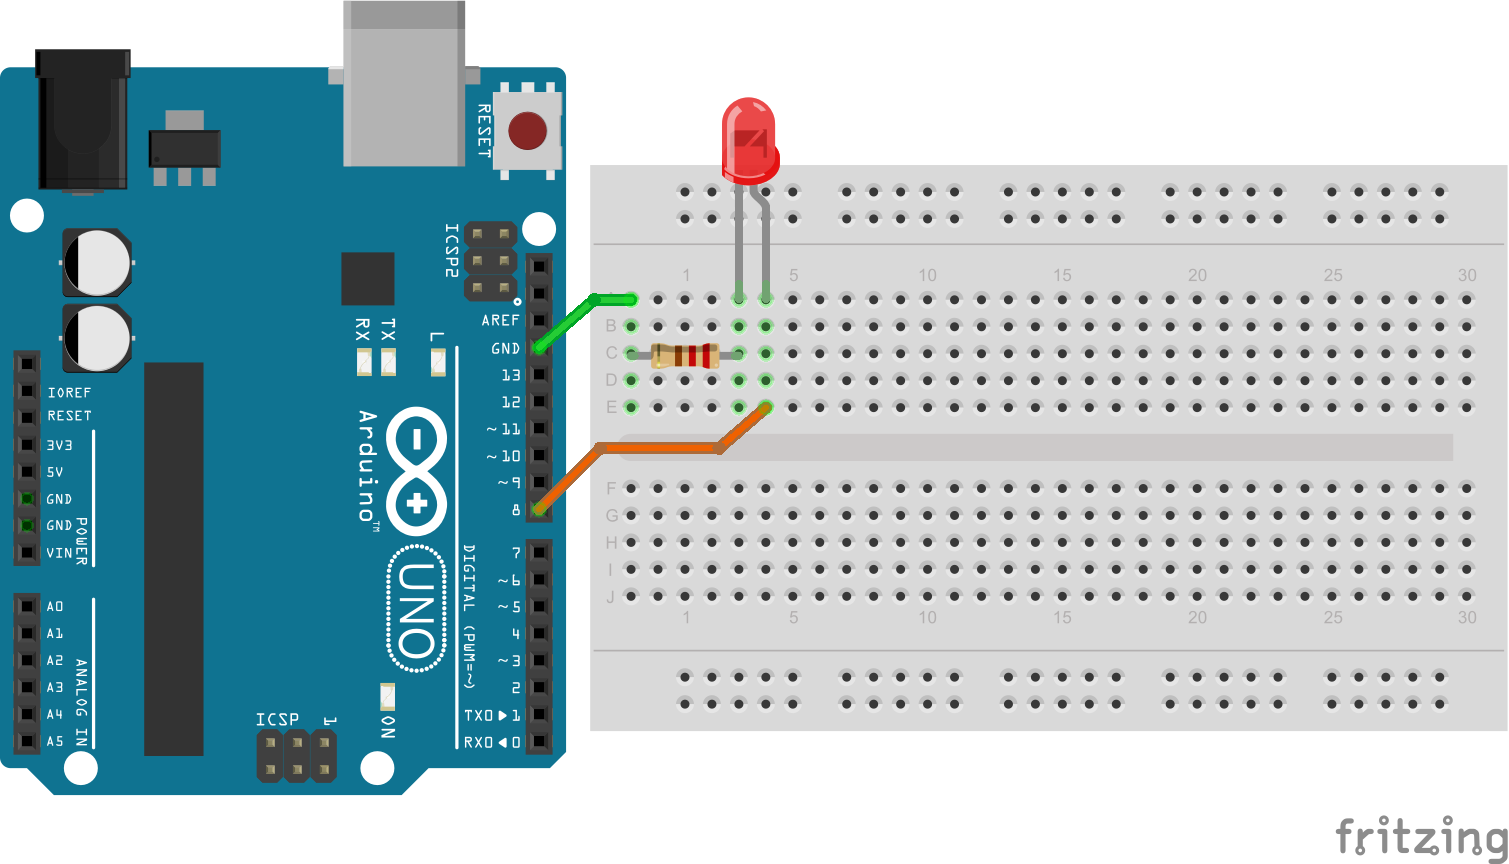
\includegraphics[scale=0.7]{circ1.png}
\caption{Circuito para encender un led conectado al pin 8.\label{circ}}
\end{figure}

Cabe notar que la imagen del circuito, fue desarrollada en el software open-source \emph{Fritzing}, en donde se muestra una protoboard con los componentes posicionados en ella. A nivel profesional, los circuitos no se muestran de esa manera sino que se representan por medio de diagramas como el mostrado en la figura \ref{diagrama1} y puede ir de muchas formas sobre la protoboard que no es más que un conjunto de conductores ordenados. (véase la figura \ref{protoboard} tomada de \cite{SIK})

\begin{figure}[h]
\centering
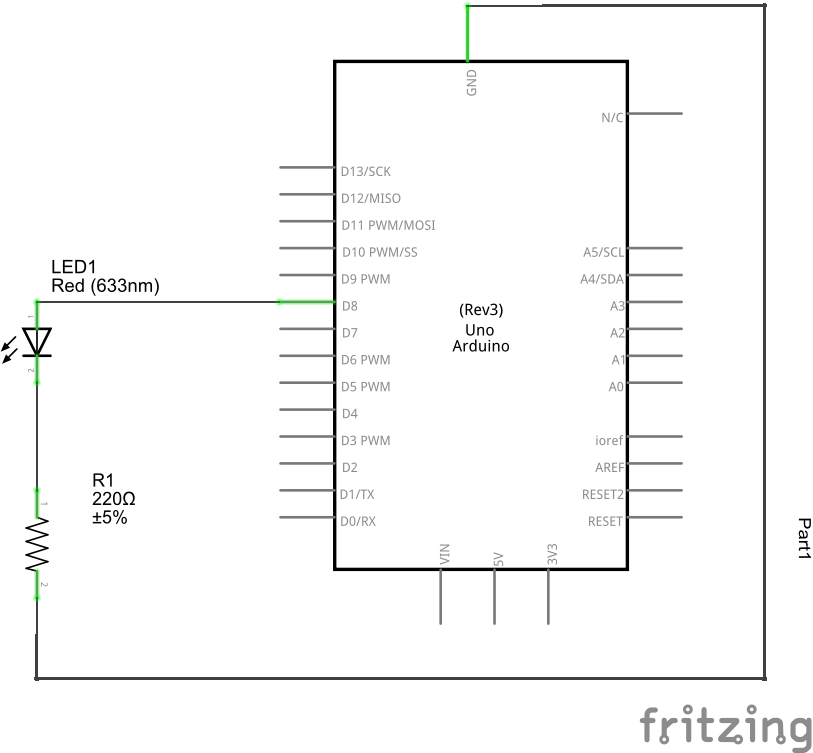
\includegraphics[scale=0.9]{diagrama1.png}
\caption{Diagrama de cicuito de la Actividad 1. \label{diagrama1}}
\end{figure}

\begin{figure}
\centering
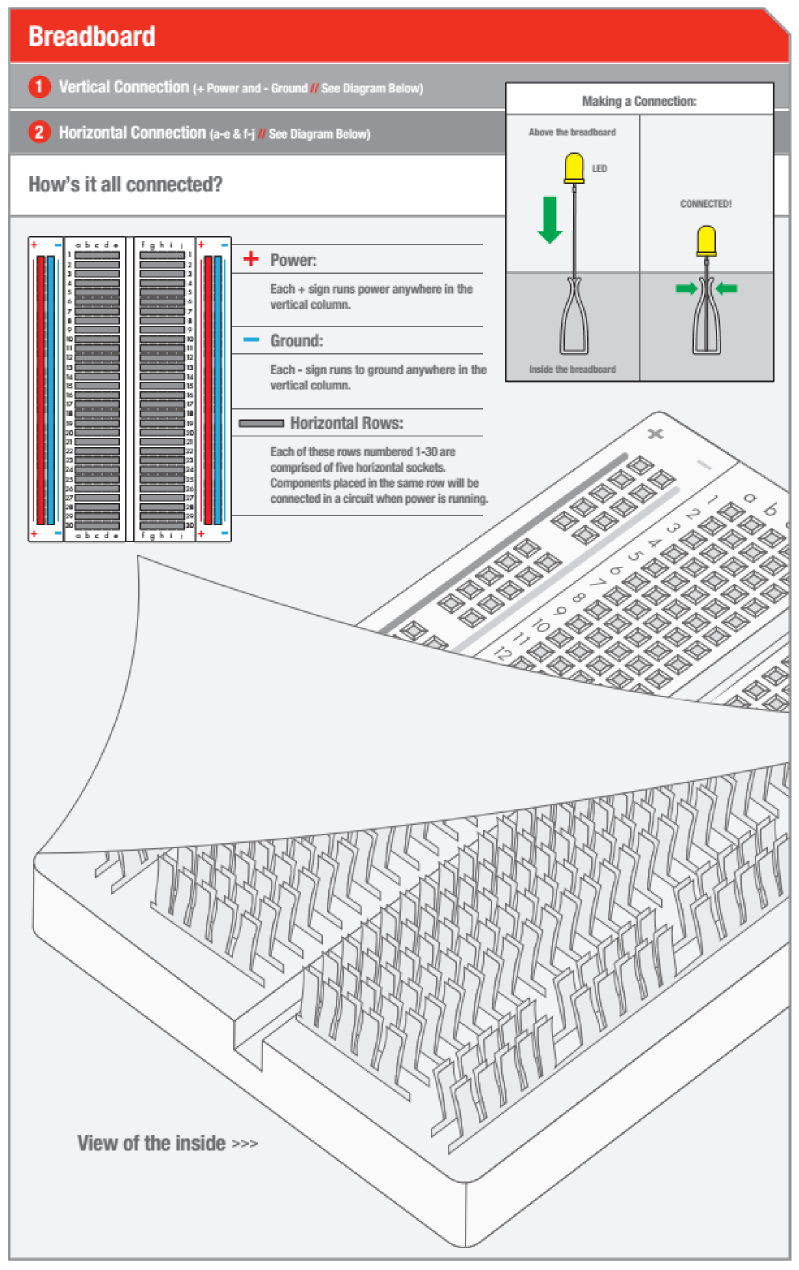
\includegraphics[scale=0.7]{protoboard.png}
\caption{Infografía acerca de la protoboard. \cite{SIK} \label{protoboard}}
\end{figure}

\newpage

\section{Control de entradas Digitales}

Entrada digital, quiere decir que nuestra Arduino será capaz de monitorear una señal eléctrica y realizar alguna acción en cuanto esto ocurra. La instrucción clave aquí es la siguiente:

\begin{itemize}
\item \texttt{digitalRead(3)}\\
Retorna el valor del estado del pin 3, que puede ser \texttt{HIGH} o \texttt{LOW} e incluso ser interpretado como 0 o 1. Se debe considerar declarar previamente el pin como entrada.
\end{itemize}

A continuación, se presenta un código, que cambia el estado del led del circuito de la imagen \ref{circEntrada} al ser presionado un botón, es decir, si el led está apagado, al presionar el boton encenderá y al presionar nuevamente, se apagará.

En este código, se puede ver como es posible utilizar características y técnicas del lenguaje C, también resulta de interés el uso de la instrucción \texttt{delay(50)}, puesto que el microcontrolador trabaja a una velocidad tal que, es posible que reaccione a los rebotes que produce el botón al ser presionado, aunque nosotros no lo notemos.
\newpage
\begin{lstlisting}[style=myArduino] 
boolean  estadoLed = false;

void setup() {
  
  pinMode(8, OUTPUT);  //declaro el pin 8 como salida
  pinMode(3, INPUT);  //declaro el pin 3 como entrada

}

void loop() {
  //pregunto si se ha presionado el boton en el pin 3
  if(digitalRead(3)){
    
    delay(50);            //espero a que el boton deje de rebotar
    estadoLed=!estadoLed; //cambio el estado del flag
  
  }
  
  digitalWrite(8,estadoLed);  //escribo el valor en el pin correspondiente
                              //al led

}
\end{lstlisting}

\begin{figure}
\centering
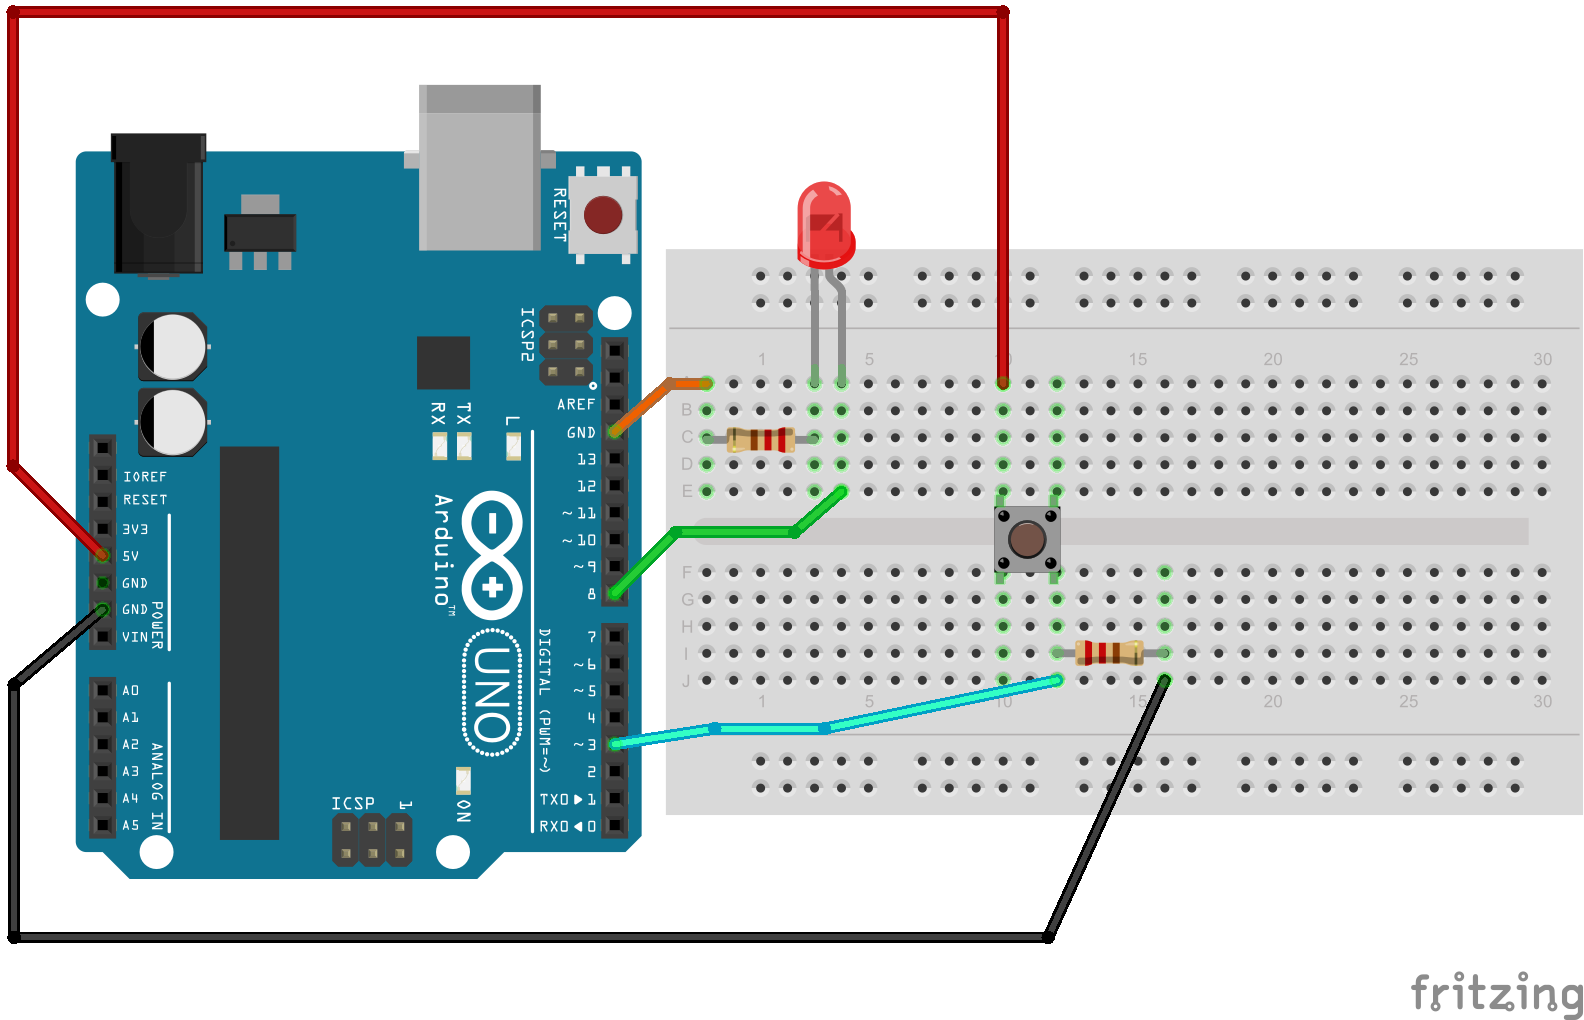
\includegraphics[scale=0.7]{botonLed.png}
\caption{Circuito para probar entrada digital del pin 3. \label{circEntrada}}
\end{figure}
 
\subsection{Actividad}
\begin{enumerate}
\item Con ayuda de su compañero/a, realice el montaje del circuito mostrado en la figura \ref{circEntrada}.
\item Cargue el programa correspondiente en su Arduino.
\item Cree un nuevo programa, tal que al presionar el botón, el led parpadee tres veces.
\end{enumerate}

\section{Control de Salidas PWM}\label{pwmSec}

\begin{center}
{\it Pulse Wide Modulation}
\end{center}

Tal como se vio en un principio, que comportamientos extraños ocurrían al exponer el led del pin 13 a encendidos y apagados demasiado rápidos, sabemos de cierta forma que controlar los tiempos de encendido y apagado de una señal eléctrica a gran velocidad, es a grandes rasgos, controlar su potencia.

Beneficiosamente, Arduino permite ejercer un control directo sobre la potencia \emph{virtual} de los pines marcados con el símbolo $\sim$ , mediante la técnica conocida como PWM \emph{Modulación por Ancho de Pulso} que consiste en controlar el balance entre los tiempos de estado alto y bajo de la señal.

La instrucción que permite realizar estas operaciones es la siguiente:
\begin{itemize}
\item \texttt{analogWrite(pin,potencia)}\\
Permite que el pin correspondiente, emita una señal a la potencia especificada como un número entre 0 y 255. Por ejemplo.\\
\begin{itemize}
	\item \texttt{analogWrite(9,255); //Pondrá el equivalente a 5 volts en el pin 9.}\\
	\item \texttt{analogWrite(5,1);   //Pondrá el equivalente a un voltaje muy pequeño en el pin 5.}
\end{itemize}
	En la figura \ref{pwm}, se muestran las formas de onda aplicada a los pines de salida, normalmente esto ocurre a una frecuencia de 32kHz.
\end{itemize}

\begin{figure}[h]
\centering
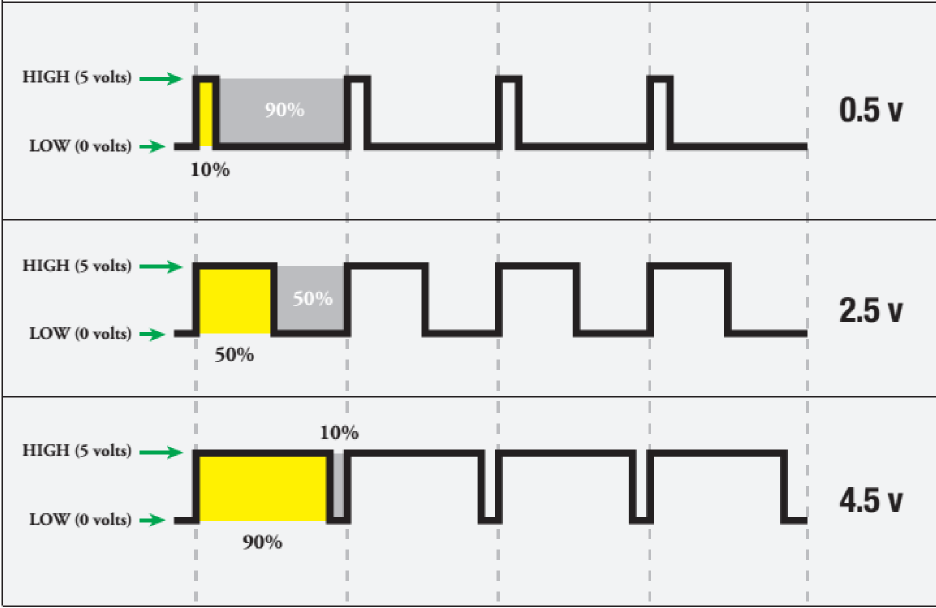
\includegraphics[scale=0.5]{pwm.png}
\caption{Señales PWM. \label{pwm}}
\end{figure}

Aunque la instrucción hace alusión a una señal analógica, resulta evidente que es solamente una aproximación digital.

\subsection{Actividad}
\begin{enumerate}
\item Utilizando el mismo circuito de la figura \ref{circEntrada}, programe el siguiente código, que permite probar la instrucción \texttt{analogWrite}, dejando el led encendido a distintos valores de potencia.

\begin{lstlisting}[style=myArduino] 
void setup() {
  
  pinMode(9, OUTPUT);  //declaro el pin 9 como salida

}

void loop() {

  analogWrite(9,100); //enciendo el pin 9 con un valor de potencia determinada 

}
\end{lstlisting}

\item Utilice sus habilidades en programación, para crear un algoritmo que varíe la intensidad del led constantemente de manera continua, como si \emph{respirara}. Recuerde que las sentencias condicionales, son las mismas del lenguaje C.

\end{enumerate}

\section{Lectura de Entradas Analógicas}

\begin{figure}[h]
\centering
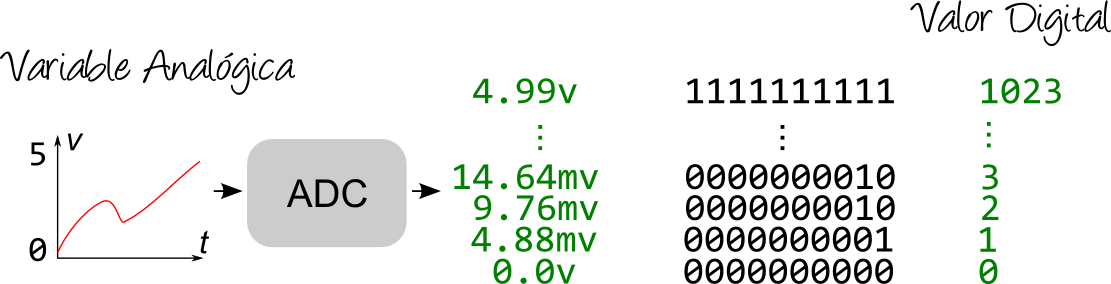
\includegraphics[scale=0.6]{adc.png}
\end{figure}

Arduino, está dotado de un conversor análogo-digital con una profundidad de 10 bits, es decir, que es capaz de transformar magnitudes analógicas entre 0 y 5 volts, en números de 0 a 1024 \emph{cuentas}. Lo anterior permite establecer que la resolución de voltaje de Arduino, es de 4.88 mili volts, lo que significa que es ese el mínimo cambio de voltaje que el sistema puede detectar.

La instrucción que nos permite capturar el número equivalente al voltaje medido es la siguiente:

\begin{itemize}
	\item \texttt{analogRead(A3)}\\
	Retorna el número de cuentas equivalente al voltaje presente en el pin A3. En total Arduino cuenta con 6 entradas analógicas, tal como se vio en la figura \ref{anatomiaArduino}. Estos pines, no necesitan ser declarados como entradas.
\end{itemize}

\subsection{Actividad}

A continuación, se presenta un programa y circuito, que lee el voltaje analógico entregado por un potenciómetro en el pin A2 y lo almacena en la variable tipo entera \texttt{medicion}. Se pide que usted realice lo siguiente:

\begin{enumerate}
	\item Realice el montaje del circuito mostrado en la imagen \ref{circuitoAnalogico}.
	
	\begin{figure}
	\centering
	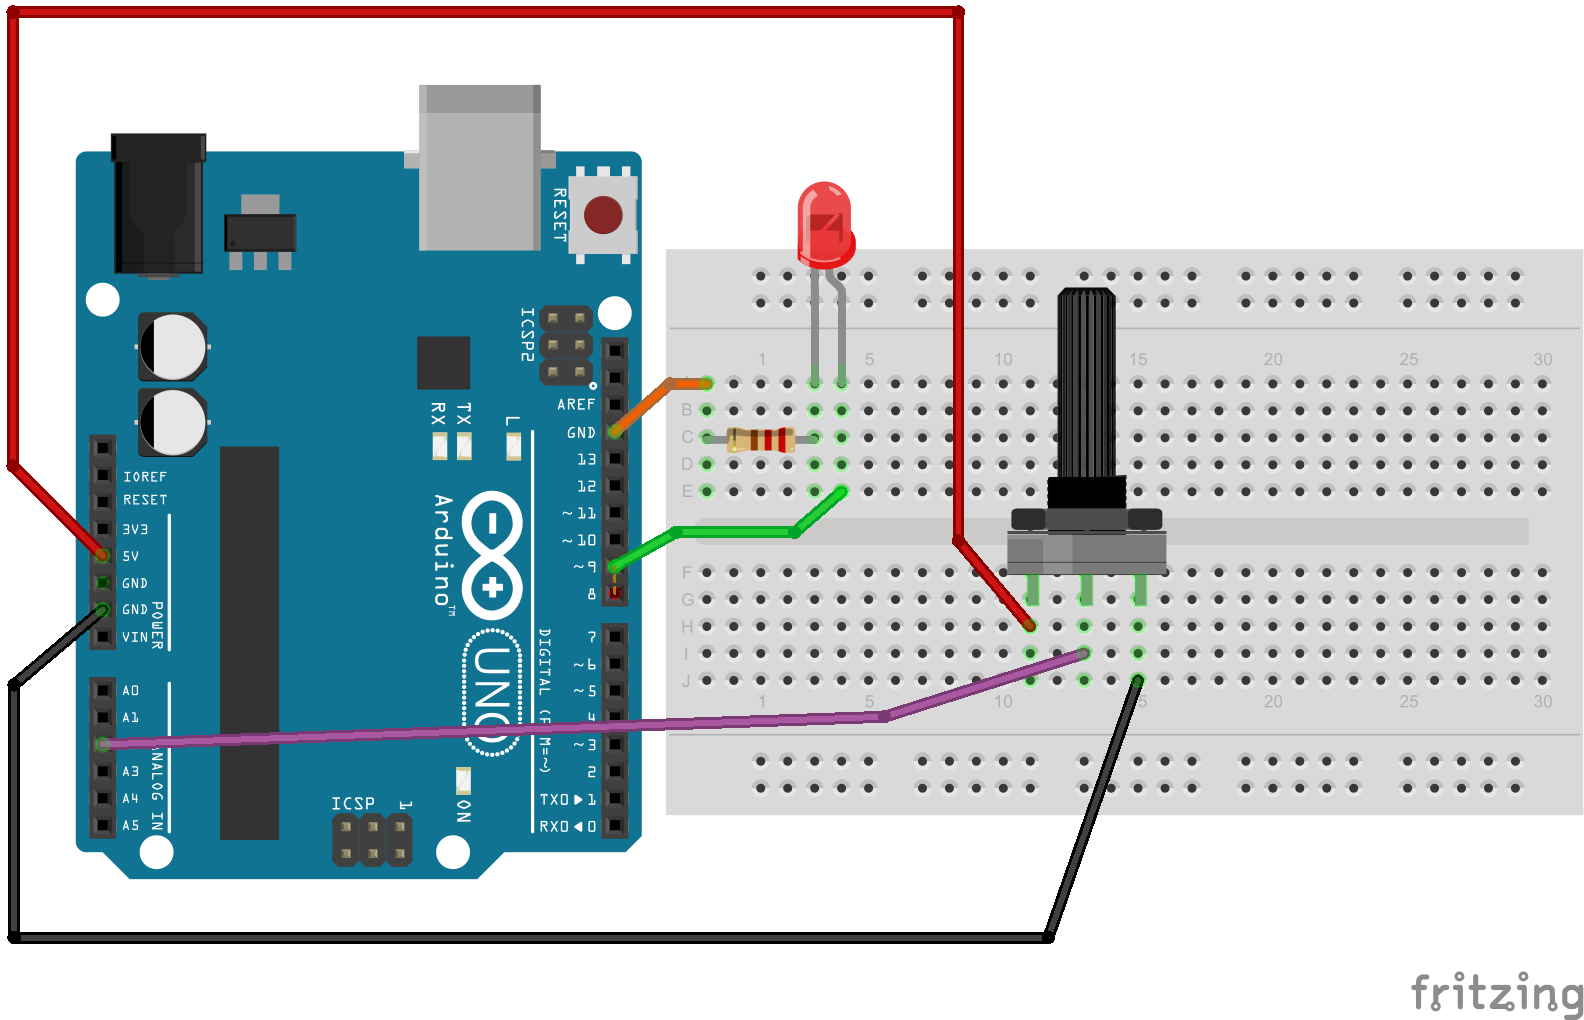
\includegraphics[scale=0.7]{circuitoAnalogico.png}
	\caption{Circuito de prueba de la actividad.\label{circuitoAnalogico}}
	\end{figure}
	
	\item Cargue el siguiente programa en su Arduino.
	
\begin{lstlisting}[style=myArduino]
int medicion;

void setup(){

}

void loop(){
	medicion=analogRead(A2);
}
\end{lstlisting}
	\item Modifique el programa presentado, de tal manera que \textbf{si el valor medido, sobrepasa las 500 cuentas, se debe encender el led.}
	
	Cabe notar que en este caso, el encendido del led será una alarma indicadora del sobrepaso del la medición por algun valor determinado.
\end{enumerate}

\section{Comunicación Serial}

En Arduino, la comunicación serial, tiene la función principal de cargar programas al microcontrolador, pero tambien puede ser usada para enviar y recibir mensajes en forma de texto ASCII entre el PC, la tarjeta e incluso algún otro dispositivo que permita este tipo de comunicación, cómo modulos de comunicación y GPS's, entre otros.  
\begin{figure}
\centering
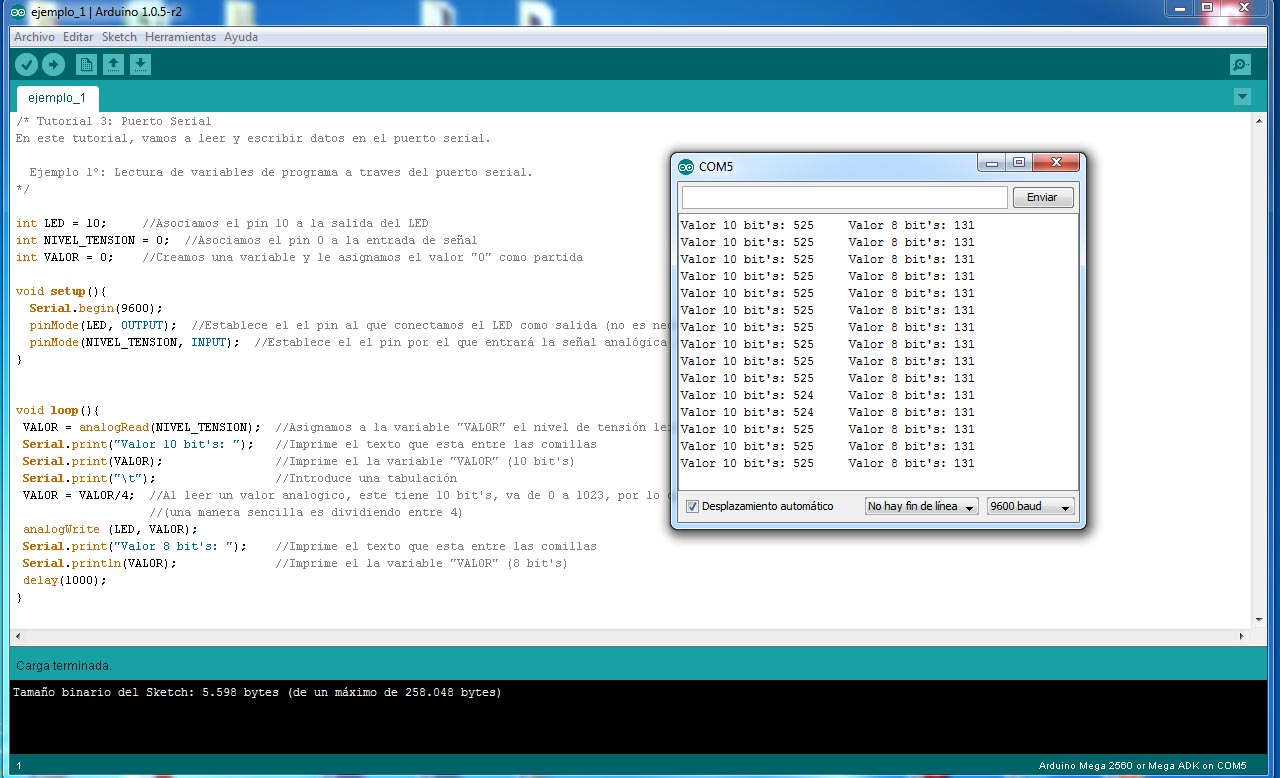
\includegraphics[scale=0.25]{serialcom.jpg}
\caption{Ventana del Monitor Serial.\label{serialcom}}
\end{figure}

Una de las maneras más simples de experimentar con la comunicación serial, es el envío y recepción de mensajes a través del \emph{Monitor Serial} que el software trae incorporado.

Las instrucciones relevantes, para manejar este tipo de comunicación son:
\begin{itemize}
\item \texttt{Serial.begin(9600)}\\
Inicia la comunicación serial a la velocidad en baudios\footnote{Bits por Segundo} especificada. La práctica habitual es utilizar esta instrucción en el \texttt{setup()}.

\item \texttt{Serial.print("mensaje")}\\
Envía la palabra \texttt{mensaje} desde Arduino al PC, mostrandose en el Monitor Serial.

\item \texttt{Serial.println("mensaje")}\\
Realiza lo mismo que la instrucción anterior, pero esta vez añade un retorno de carro al final del mensaje, es decir que si se escribe luego de esta instrucción, los mensajes continuarán en la línea siguiente, no asi en el caso anterior, donde los mensajes se van acumulando hacia el lado.

Cabe notar que ambas instrucciones, aceptan como argumentos, variables tipo \texttt{int}, \texttt{float}, entre otras y muestran su valor resultante en como caracteres ASCII.

\item \texttt{Serial.available()}\\
Retorna la cantidad de bytes almacenados en el buffer de entrada. Básicamente si este valor es distinto de cero, quiere decir que están llegando datos por el puesto serial en Arduino.

\item \texttt{Serial.read()}\\
Retorna el primer byte disponible en el buffer, una vez leído pasa al siguiente byte. Cabe notar que los datos vienen en binario correspondiente al código ASCII del caracter entrante.

\item \texttt{Serial.parseInt()}\\
Retorna el valor entero que se pueda identificar en el buffer de entrada, resulta muy útil para leer variables de entrada y almacenarlas como dato entero. Cabe notar que cuando no recibe datos retorna el valor entero cero.
\end{itemize}

Existen más instrucciones para el puerto Serie y se pueden encontrar en el sitio de referencia para la clase Serial del en la página oficial de Arduino. \cite{Serial} 

\subsection{Actividad: Lectura de variable analógica desde el Puerto Serie }\label{puertoSerie}
A continuación, presenta un código que permite leer valor del potenciómetro de la actividad anterior, almacenarlo en un variable de tipo entera y enviar ese valor de manera que se pueda visualizar a través del Monitor Serial.

\begin{lstlisting}[style=myArduino]
int medicion;

void setup(){
	Serial.begin(9600);
}

void loop(){
	medicion=analogRead(A2);
	
	Serial.print("Valor Medido: ");
	Serial.println(medicion);
	delay(200);
}
\end{lstlisting} 

Cabe notar, que en el código se utiliza un delay para no saturar el Monitor Serial con mensajes a gran velocidad.

\begin{enumerate}
\item Cargue el programa mostrado en su Arduino y mueva el potenciómetro para verificar el correcto funcionamiento de la aplicación.

\item Modifique el programa anterior, de manera que se muestre a través del Monitor Serial el valor de \textbf{voltaje} que se está midiendo en la entrada.

\begin{center}
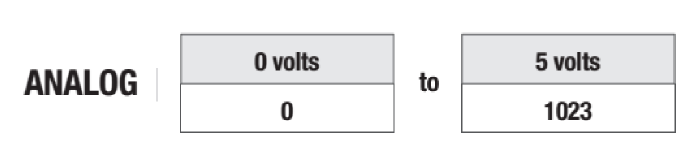
\includegraphics[scale=0.5]{anValue.png}
\end{center}

En instrumentación industrial, está operación se conoce como \emph{Escalamiento} y es habitual que los sistemas de control como PLC's la realicen, puesto que la mayoría de los instrumentos de medición entregan una señal en corriente de 4 a 20ma. la que debe ser transformada a la variable original de medición.
\end{enumerate}

\subsection{Actividad: Envío de instrucciones a Arduino a través del Puerto Serie}
A continuación, presenta un código que permite enviar una instrucción a Arduino a través del Puerto Serie, de manera que se le ordene el encendido o apagado de un Led. Se utiliza el mismo circuito de la figura \ref{circuitoAnalogico}.

\begin{lstlisting}[style=myArduino]
int byteEntrante;      	// aqui guardamos el valor que 
						//entra en el puerto serie

void setup()
{
	//se inicia la comunicacion Serial
    Serial.begin(9600);
    //se declara el pin para el led como salida
    pinMode(9, OUTPUT);
}

void loop()
{
    // se esperan datos en el puerto serie
    if (Serial.available() > 0)
    {
        // leemos el primer byte del buffer
        byteEntrante = Serial.read();
        // si llega una H encendemos el led
        if (byteEntrante == 'H')
        {
            digitalWrite(9, HIGH);
        }
        // si llega una L lo apagamos
        if (byteEntrante == 'L')
        {
            digitalWrite(9, LOW);
        }
    }
}
\end{lstlisting} 

\begin{enumerate}
\item Cargue el programa mostrado en su Arduino y verifique el correcto funcionamiento de la aplicación.

\item Modifique el programa anterior, de manera que nos confirme a través del mismo puerto serial si el led está encendido o apagado y si enviamos algún caracter no esperado, nos indique la situación y nos recomiende ingresar \texttt{H} o \texttt{L}.
\end{enumerate}
%=================================================================================================================
\chapter{Lectura de Sensores y Control de Actuadores con Arduino.}

Una de las características de los sistemas como arduino, es que pueden interactuar de manera física con el mundo que nos rodea, sus creadores lo llaman \emph{Physical Computing}. Toma mediciones del entorno o proceso por medio de sensores, realiza algún tipo de procesamiento o toma de decisión y en base a ello ejerce alguna acción sobre el sistema por medio de los actuadores.

\begin{center}
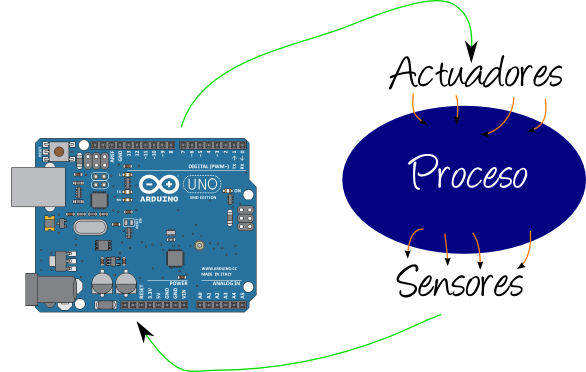
\includegraphics[scale=0.7]{proceso.png}
\end{center} 

En este capítulo, veremos algunos casos particulares de sensores y actuadores que se pueden utilizar con esta tarjeta ya sea por medio de mediciones analógicas o digitales.

\section{Sensor de luminosidad LDR}

LDR significa \emph{Light Dependant Resistor} por sus siglas en inglés, y se trata de un sensor de luz; este cambia su resistencia eléctrica dependiendo de la cantidad de luz que incida sobre el. También es común que se los llame \emph{Foto-resistencia} debido a este mismo principio.

\begin{figure}[h]
\centering
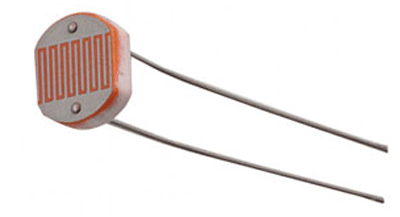
\includegraphics[scale=0.4]{LDR-Resistor.png}
\caption{Sensor de Luminosidad LDR. \label{LDR}}
\end{figure}

En la figura \ref{LDR}, se puede ver como luce este tipo de sensor. A mayor luz, el LDR disminuirá su valor resistivo, mientras que en la oscuridad presentará una gran resistencia eléctrica.

Como ya se ha visto antes, arduino sólo mide voltajes, ya se de forma digital o analógica y no mide resistencia. Gracias a ley de Ohm, estas magnitudes están ligadas y es posible generar voltajes proporcionales a las mediciones de luz por medio de un \emph{circuito divisor de tensión}, cómo el que se muestra en la figura \ref{circuitoLDR}. Cabe notar, que este principio de medición, es válido para cualquier sensor que sea del tipo resistivo, por ejemplo, sensores flex o galgas extensiométricas, sensores de carga, etc.
\begin{figure}[h]
\centering
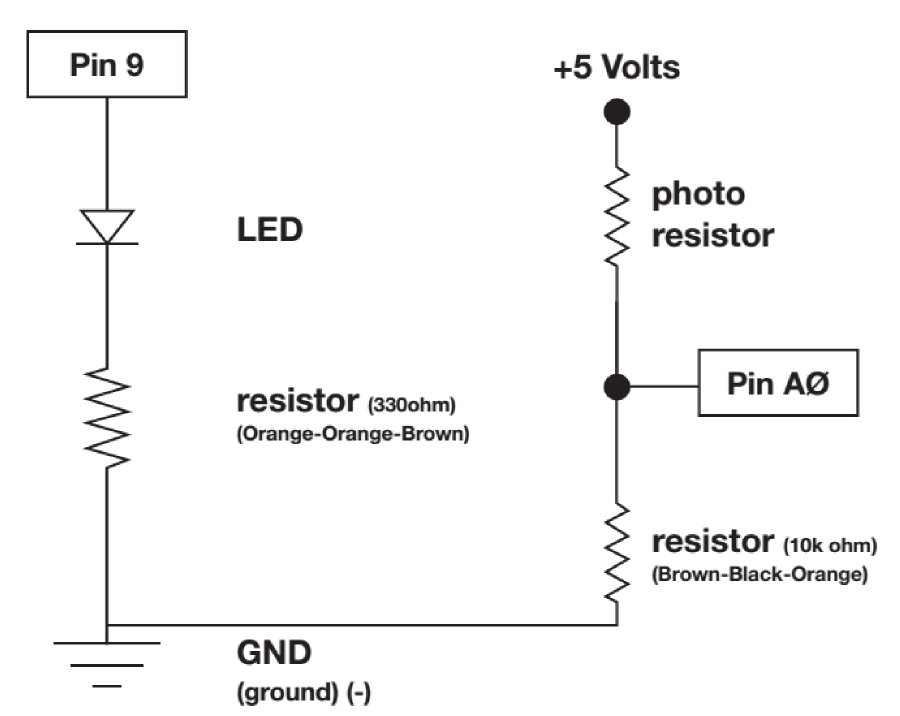
\includegraphics[scale=0.35]{circuitoLDR.png}
\caption{Divisor de tensión para medir luminosidad con un LDR.\label{circuitoLDR}}
\end{figure}

En este caso, el Led conectado al pin 9, no es necesario para la medición con LDR, pero luego programaremos para que nos indique si el nivel de luz ha bajado de algún valor determinado.

\subsection{Actividad}

\begin{enumerate}
\item Realice el montaje en protoboard, del circuito de la figura \ref{circuitoLDR}. Esta vez no se incluye el diagrama de la protoboard, pues debe ser usted quien decida el montaje.
\item Modifique el código de la Actividad \ref{puertoSerie} para poder verificar los distintos valores entregados por el sensor ante diversas condiciones de Luz, puede tapar el sensor, iluminarlo con la linterna de su teléfono y revisar su comportamiento.

\item Defina niveles de Luminosidad para una sala iluminada y una sala oscura, en base a eso, programe el Arduino para que encienda automáticamente un led al detectar que la sala está oscura.
\end{enumerate}

\section{Sensor de Temperatura LM35}

El sensor LM35, está diseñado para medir temperaturas entre 0 y 150$^{\circ}$C aproximadamente, internamente contiene circuitería analógica perfectamente calibrada para asegurar una precisión máxima de 0.5$^{\circ}$C dentro de ese rango.

\begin{figure}[h]
\centering
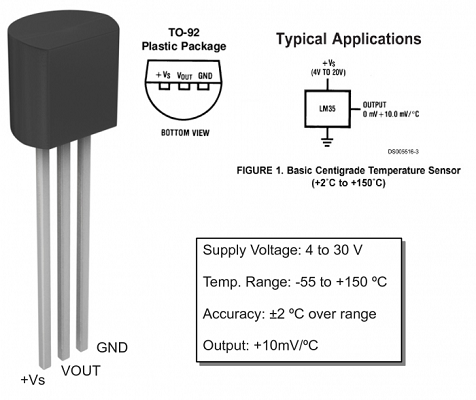
\includegraphics[scale=0.55]{lm35.png}
\caption{Sensor LM35, pines del dispositivo. \label{LM35}}
\end{figure}

A su salida, entrega una señal de voltaje proporcional a la medición de temperatura con característica de {\bf 10mV por cada Grado Celsius} según su hoja de especificaciones técnicas. \cite{LM35}

En este caso, es necesario realizar el escalamiento, para que en el puerto serial nos muestre el valor de temperatura en vez del número de cuentas correspondiente a la medición.

\subsection{Actividad}
\begin{enumerate}
\item Considerando que el sensor entrega una medida equivalente  10 mili-volts por cada grado medido, esto es 0 volts a 0$^\circ$C y a los 5 volts estaría mostrando 500$^\circ$, matemáticamente hablando; realice el cálculo que debe ser implementado en arduino para que este muestre a través del puerto serial, el valor de temperatura medido.

\item Conecte el sensor de temperatura a la entrada analógica A0 de Arduino de acuerdo a las especificaciones del fabricante--figura \ref{LM35}--, registre también el diagrama de dicha conexión.

\item Programe el microcontrolador, de manera que al abrir el puerto serial este muestre los valores de temperatura como sigue:
\begin{center}
	\texttt{TEMPERATURA: 23.0 Grados}\\
	\texttt{TEMPERATURA: 23.5 Grados}
\end{center}

\item Establezca un indicador de alarma al sobrepasar los 50$^\circ$C, mediante un Led conectado al Pin 9 de su Arduino.
\end{enumerate}

\subsection{Serial Plotter}

El Software Arduino Incorpora en sus últimas versiones una utilidad llamada \emph{Serial Plotter}, que permite graficar variables en tiempo Real, en la pantalla del ordenador. Serial Plotter, necesita recibir números separados por comas, para poder mostrarlos, si recibe texto, no mostrará nada.
Pruebe el Serial Plotter con el sensor LM35 y el último programa de la actividad.

\begin{figure}[h]
\centering
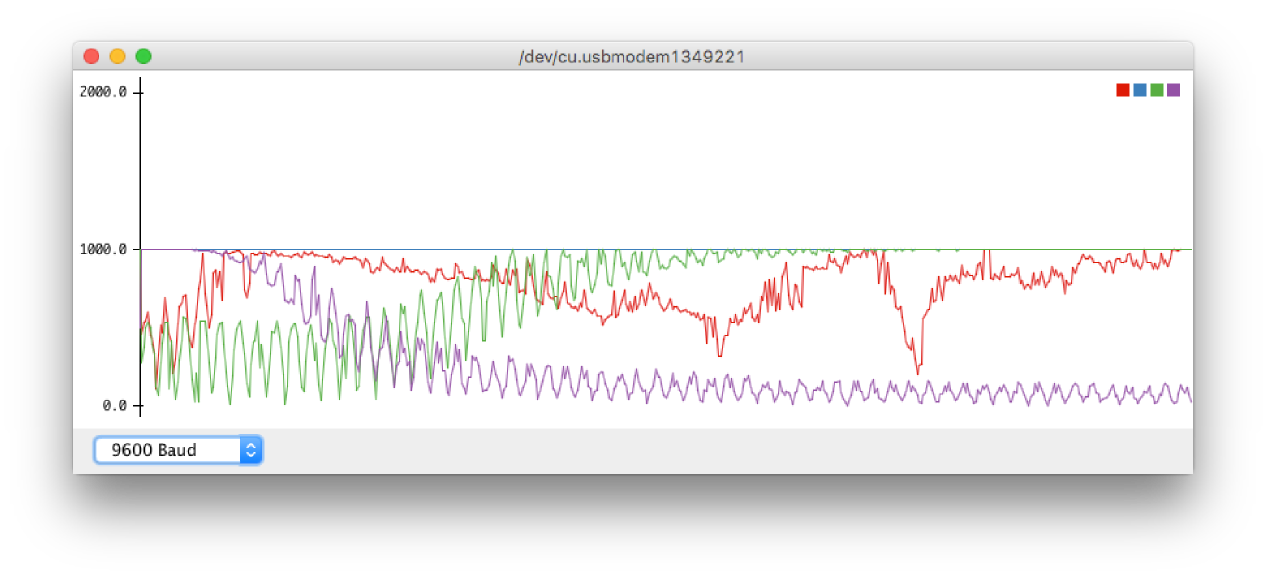
\includegraphics[scale=0.4]{serialPlotter.png}
\caption{Serial Plotter de Arduino IDE.}
\end{figure}

\section{Sensor Ultrasónico Parallax PING}\label{pingSec}

El sensor ultrasónico Ping, permite medir distancias mediante el envío de un pulso de ultrasonido y el conteo del tiempo de vuelo del pulso hasta recibirlo de vuelta.

\begin{figure}[h]
\centering
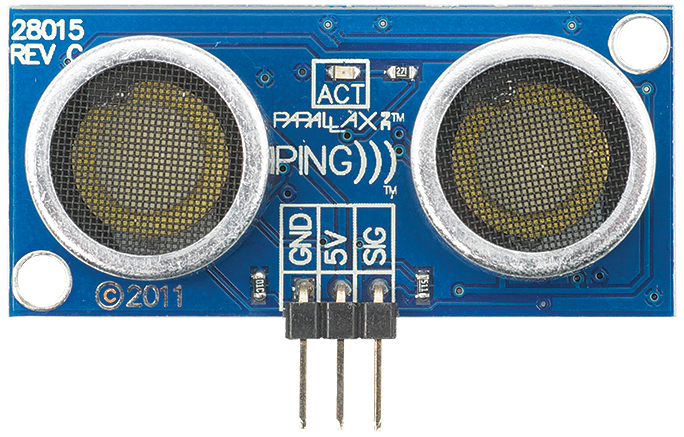
\includegraphics[scale=0.3]{ping.jpg}
\caption{Sensor Ultrasónico Parallax Ping.\label{ping}}
\end{figure}  

Al tener un objeto sólido en frente, la onda ultrasónica rebotará y será recibida con una diferencia de tiempo proporcional a la distancia a la que se encuentra el objeto, cabe notar que el pin que se usa tanto como para emitir, como recibir el ultrasonido es el mismo, por lo tanto el microcontrolador debe ser capaz de cambiar su configuración de entrada a salida durante la marcha. Este sensor fue desarrollado inicialmente para complemetar un kit de robótica educacional llamado \emph{Boe-Bot} basado en el microcontrolador \emph{Basic Stamp}, hoy en día es usado muchas aplicaciones que van desde la robótica hasta la IoT ya que es perfectamente compatible con Arduino.

\begin{figure}[h]
\centering
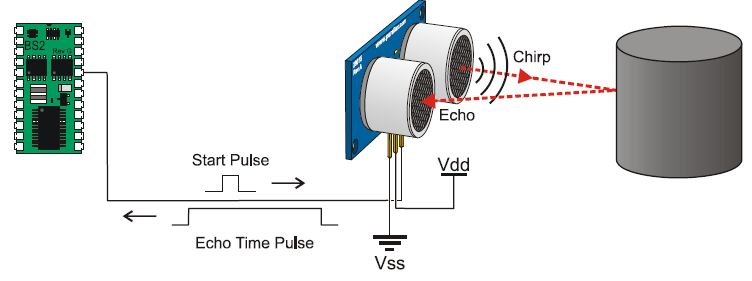
\includegraphics[scale=0.4]{medicionPing.JPG}
\caption{Medición con Sensor Ping y Microcontrolador Basic Stamp}
\end{figure}

La realizar mediciones reiteradas con este sensor, requerirá que el controlador execute por lo menos los siguientes pasos, de forma repetitiva:
\begin{enumerate}
\item Declarar el pin \texttt{Sig} como \textbf{Salida}.
\item Emitir un pulso con una duración de 5 micro segundos.
\item Declarar el pin \texttt{Sig} como \textbf{Entrada}.
\item Contar el tiempo hasta que se recibe el pulso ultrasonico y guardarlo en una variable, este sera el \emph{Tiempo de Vuelo}. 
\end{enumerate}

Finalmente, el tiempo de duración será proporcional a la distancia. En base a la velocidad del sonido de 340 metros por segundo o 29 microsegundos por centimetro, es posible establecer que el pulso ultrasónico va y vuelve, luego para encontrar la distancia hasta el objeto, necesitamos la mitad de la distancia recorrida.

\begin{center}
\texttt{distancia = tiempoVuelo / 29 / 2;}
\end{center}

A continuación, se presenta un código que toma la medición del sensor Ping y muestra el valor de la distancia en centímetros a través del puerto serial.

\begin{lstlisting}[style=myArduino]
long tiempoVuelo, distancia;
const int pingPin = 7;	// pin Sig del sensor


void setup() {
  // inicio de la comunicacion Serial
  Serial.begin(9600);
}

void loop() {

  // Se declara el pin como salida
  pinMode(pingPin, OUTPUT);
  
  // Se forma el pulso de 5 microsegundos
  digitalWrite(pingPin, LOW);
  delayMicroseconds(2);
  digitalWrite(pingPin, HIGH);
  delayMicroseconds(5);
  digitalWrite(pingPin, LOW);

  // se declara el pin como entrada
  pinMode(pingPin, INPUT);
  
  tiempoVuelo = pulseIn(pingPin, HIGH);

  // calculamos el valor en CM 
  distancia = tiempoVuelo / 29 / 2;

  // se muestra el resultado	
  Serial.print("Distancia: ");
  Serial.println(distancia);

  delay(100);
}
\end{lstlisting}

\subsection{Actividad}

\begin{enumerate}
	\item Realice el conexionado del sensor a su tarjeta arduino.	
	\item Programe el microcontrolador y verifique el correcto funcionamiento de la aplicación.
	\item Modifique el código de forma que pueda ser utilizado con el Serial Plotter. Comente acerca de la fidelidad de la señal mostrada y el ruido presente en esta.
	\item Implemente un código, tal que cada 10 mediciones arduino muestre el promedio de estas, con el fin de obtener una medición más suave.
\end{enumerate}

\section{Pantalla LCD 16x2}\label{LCD}

\begin{figure}[h]
\centering
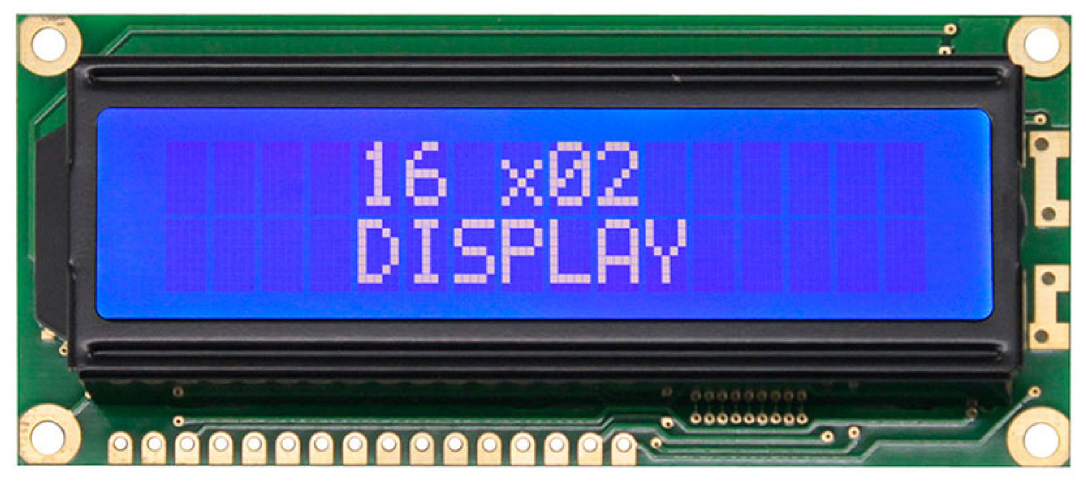
\includegraphics[scale=0.3]{lvcd.png}
\caption{Pantalla Lcd 16x2.\label{lcd}}
\end{figure}

Se trata de un periférico bastante popular, que aún se puede encontrar en algunos equipos comerciales e industriales. Por ejemplo, estas maquinas expendedoras, de Inacap Concepción.

\begin{figure}[h]
\centering
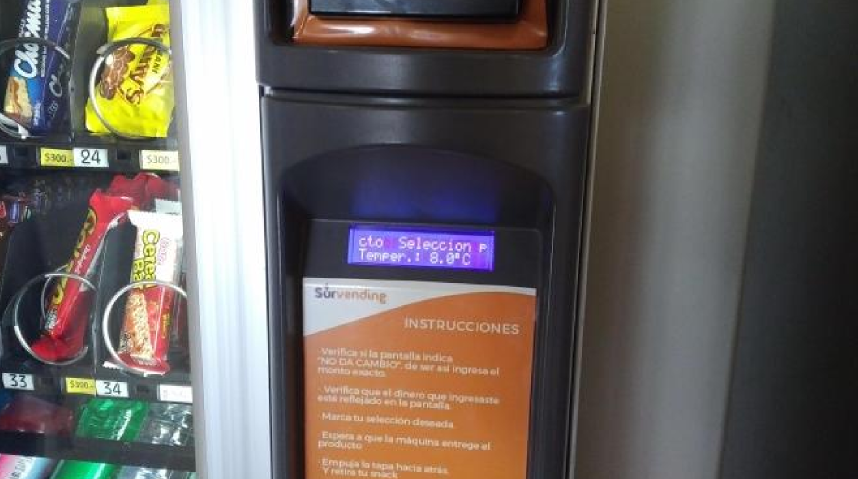
\includegraphics[scale=0.5]{lcd_maquina.png}
\caption{Utilización de pantalla Lcd en Vending-Machine.\label{lcd}}
\end{figure}

Estas pantallas utilizan un driver HD44780 creado el año 1987, en ese entonces, algo equivalente a lo que hoy sería el procesador de un monitor de ordenador.

El trabajo que hace este micro, no es menor, puesto que se encarga de encender o apagar cada uno de los pequeños cuadrados que componen cada caracter de nuestra pantalla. Una ardua tarea, si pensamos en que cada uno de estos puntos utilizaría una salida de nuestro un microcontrolador como Arduino, obviamente no sería posible.

\begin{figure}[h]
\centering
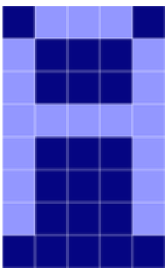
\includegraphics[scale=0.4]{matriz.png}
\caption{Matriz de puntos que forma un caracter.}
\end{figure}

El producto, consta de una interfaz sencilla, mostrada en la figura \ref{interfaz}, es universal casi a todas las pantallas LCD 16x2 e incluso otras variantes como 16x4 o alguna otra basada en el mismo driver.

\begin{figure}[h]
\centering
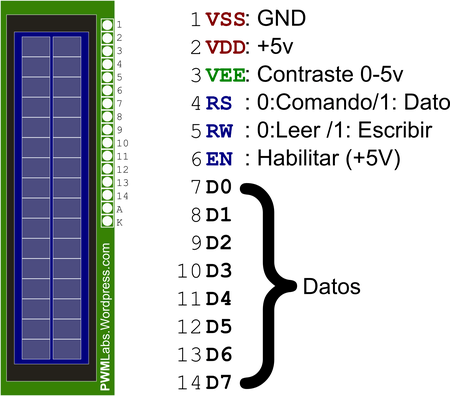
\includegraphics[scale=2]{lcd_pines.png}
\caption{Interfaz de conexión de una pantalla Lcd 16x2.\label{interfaz}}
\end{figure}

Aunque, son muchos pines, la conexión es bastante simple, y podemos dividirla, en:
\begin{itemize}
	\item {\bf Pines Alimentación:} VSS, VDD.
	\item {\bf Contraste:} Conectamos un Potenciómetro de 10k y con el manipulamos para una pantalla más clara u oscura.
	\item {\bf Control:} RS y EN son los pines que usará Arduino para manejar la pantalla. RW sirve para enviar el dato de vuelta, pero en este caso eso es innecesario asi que se conecta a GND.
	
	\item {\bf Datos:} En este Byte, Arduino, enviará los datos o comandos. Aunque son 8 lineas desde el nuestra tarjeta hasta la pantalla, nuestra librería funciona sólo con 4 bits. D4 , D5, D6 y D7, por lo tanto, los demás pines se aterrizan.
\end{itemize}

En resumen, además de la alimentación, el contraste y aterrizar los pines que no se utilizan; se deben conectar a salidas de Arduino, los pines RS, EN, D4, D5, D6 y D7. 

Enviar los datos ASCII en hexadecimal hasta la pantalla resulta una tarea un tanto ardua de programar, por lo cual, se hace uso de una librería de terceros, en este caso se utilizaremos \texttt{LiquidCrystal}, que en las últimas versiones ha pasado a ser parte de las librerías oficiales que Arduino trae en sus repositorios.

\subsection{Instalación de Librerias}\label{library}

Para instalar una nueva librería en Arduino IDE, debe dirigirse a \texttt{Sketch>Include Library>Manage Libariess}, como se muestra en la figura \ref{linInstall}.

\begin{figure}[h]
\centering
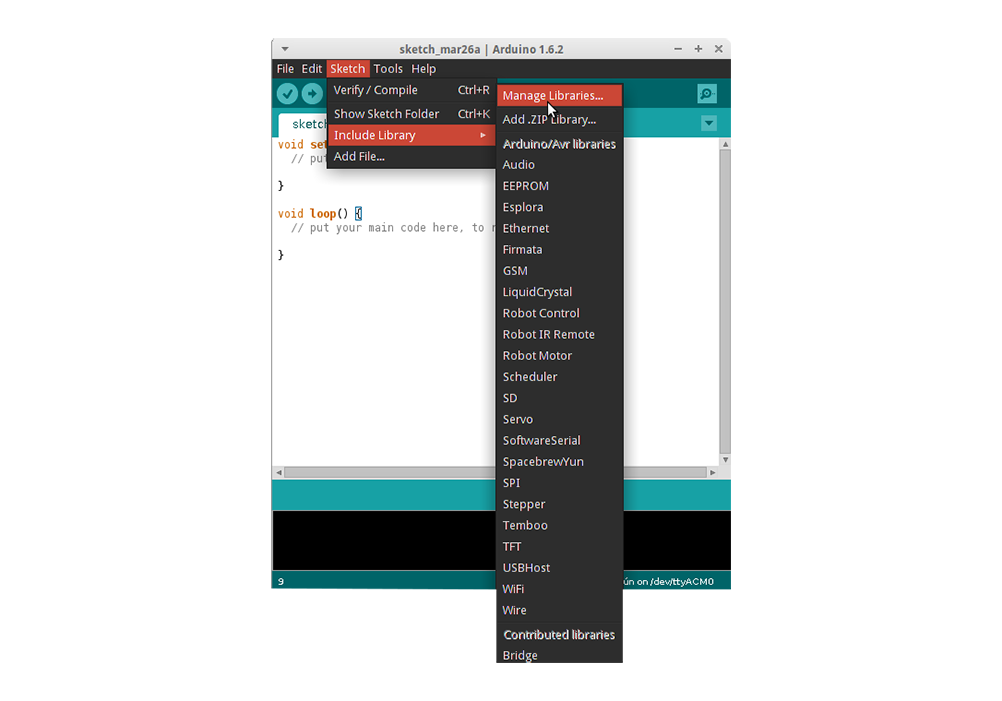
\includegraphics[scale=0.5]{LibraryManager_1.png}
\caption{Acceso al \emph{Library Manager} en Arduino IDE. \label{linInstall}}
\end{figure}

Una vez abierta la ventana \emph{Library Manager}. Se despliega un listado con las librerías añadidas oficialmente a los repositorios de Arduino, en el buscador agregamos \emph{LiquidCrystal} y debería aparacer nuestra librería con un botón para instalar, presionamos dicho boton y seguimos el proceso. En la figura \ref{libMan}, se muestra la ventana del Library Manager, que en este caso no muestra el boton para instalar \emph{LiquidCrystal}, pues ya está instalado en ese equipo.

\begin{figure}[h]
\centering
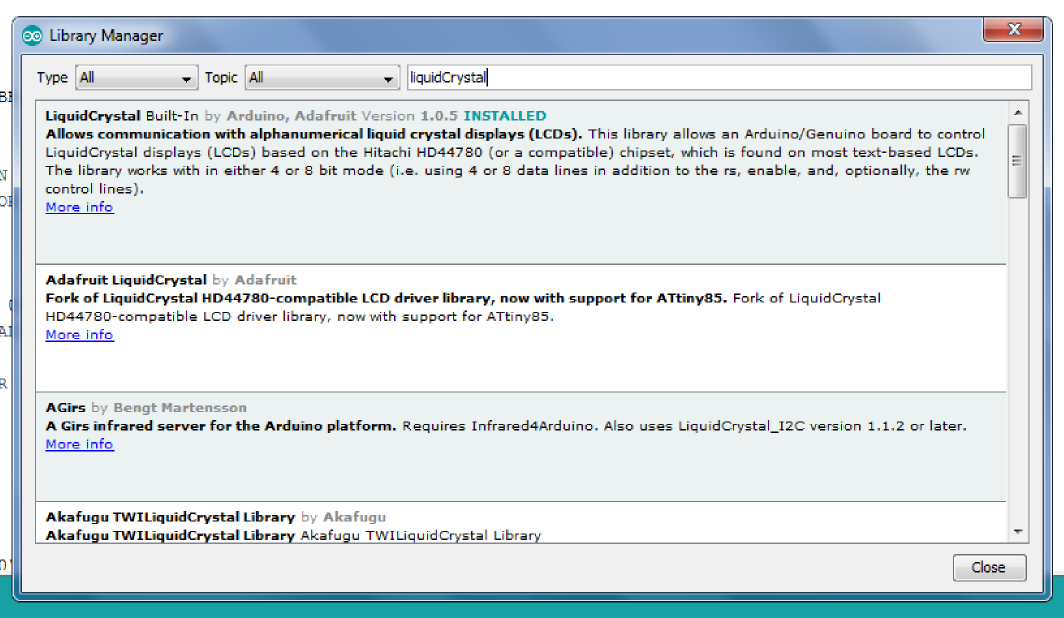
\includegraphics[scale=0.5]{libManager.png}
\caption{Ventana del \emph{Library Manager}.\label{libMan}}
\end{figure}

\subsection{Programación de Pantalla LCD}\label{lcdprog}

A continuación, se provee un programa de ejemplo que muestra en la pantalla Lcd el mensaje \emph{''Hello World"} y bajo este un contador que indica los segundos transcurridos desde el inicio del programa.

La instrucción \texttt{millis()}, retorna la cantidad de milisegundos que han transcurrido desde el último reset o encendido de la tarjeta, esta instrucción resulta muy útil para operaciones que requieren contar o controlar el tiempo en que se ejecuta una actividad.
\\
\begin{lstlisting}[style=myArduino]
// declaracion de pines para el LCD
const int rs = 12, en = 11, d4 = 5, d5 = 4, d6 = 3, d7 = 2;

// Creacion del objeto LCD
LiquidCrystal lcd(rs, en, d4, d5, d6, d7);

void setup() {
  // Inicializacion de un LCD 16 columnas y 2 filas
  lcd.begin(16, 2);
  
  // Esribe el mensaje en la pantalla del LCD
  // En la Posicion 0,0
  lcd.print("hello, world!");
}

void loop() {
  // ponemos el cursor en la columna 0, fila 1
  // linea 1 es la segunda fila, comienzan en 0:
  lcd.setCursor(0, 1);
  
  // muestra un conteo de tiempo:
  lcd.print(millis() / 1000);
}
\end{lstlisting}


\subsection{Actividad}

\begin{enumerate}
\item Realice la conexión de la pantalla Lcd a la placa Arduino de acuerdo a la figura \ref{circuitoLCD}, no olvide considerar el potenciómetro de $10k\Omega$, este le permitirá ajustar el brillo de la pantalla.

\begin{figure}[h]
\centering
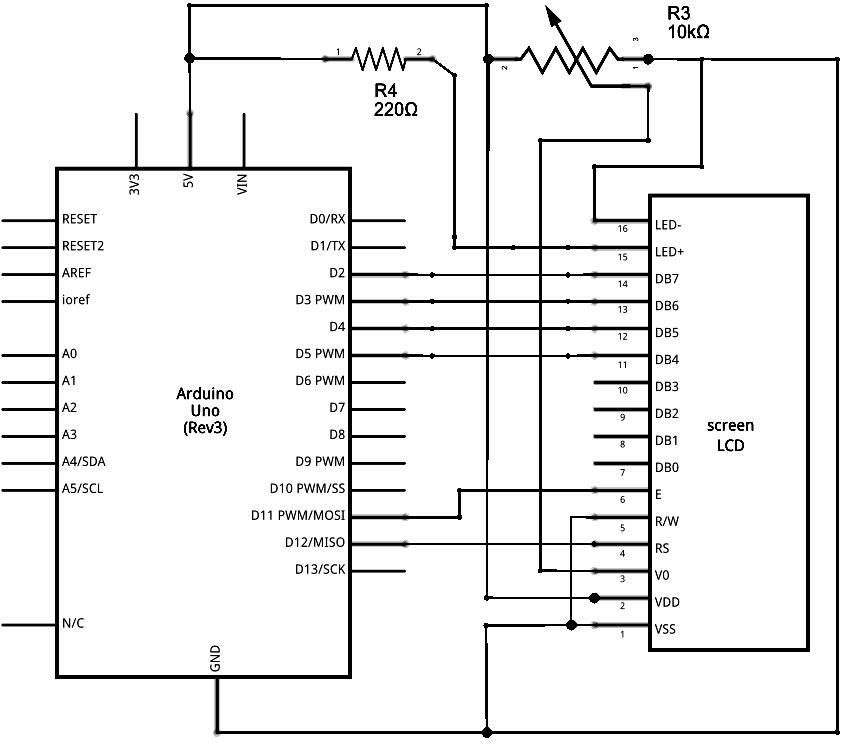
\includegraphics[scale=0.9]{circuitoLCD.png}
\caption{Conexión de Pantalla Lcd a Arduino.\label{circuitoLCD}}
\end{figure}

\item Cargue el programa de la subsección \ref{lcdprog} en su Arduino y verifique el correcto funcionamiento del ejemplo.

\item Modifique el código y circuito de forma que esta vez se pueda mostrar en pantalla, la medición de algún sensor de su elección, de los vistos en este curso. (véase el ejemplo de la figura \ref{ejemplo})

\begin{figure}[h]
\centering
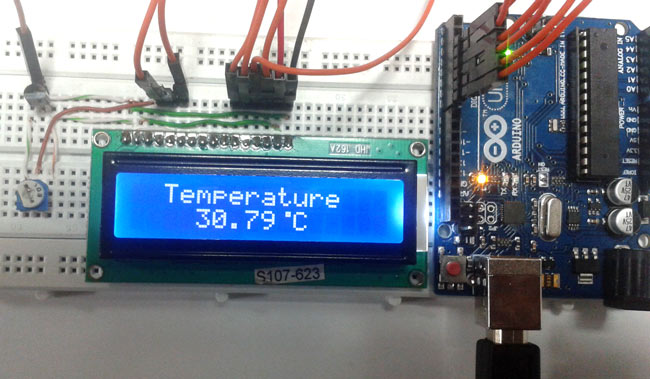
\includegraphics[scale=0.4]{ejemplo.jpg}
\caption{Ejemplo de aplicación con Sensor LM35 y Pantalla Lcd.\label{ejemplo}}
\end{figure}

\end{enumerate} 

\section{Control de Servomotores}

\begin{figure}[h]
\centering
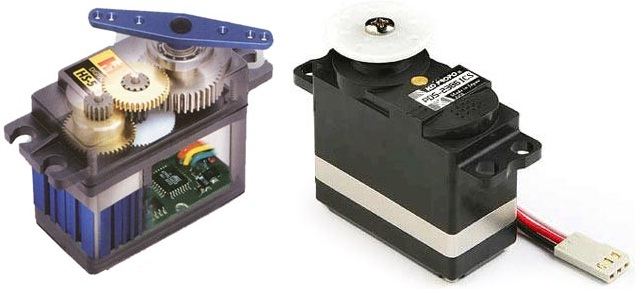
\includegraphics[scale=0.4]{servomotores.jpg}
\caption{Interior de un Servomotor.\label{servo}}
\end{figure}

El concepto de \textbf{Servo-Motor}, consiste en un sistema de control rotacional de velocidad o posición, que se caracteriza habitualmente, por traer integrado en un sólo producto --figura \ref{servo}--, al menos los siguientes elementos:
\begin{enumerate}
	\item Motor DC.
	\item Caja reductora.
	\item Sensor de Posición o Velocidad.
	\item Circuito analógico de control proporcional.
\end{enumerate} 

Al contrario de cualquier motor convencional, que gira libremente en algún sentido al ser alimentado, estos motores pueden entregar con mediana precisión, ángulos o velocidades determinadas, en base a una señal de comando, que generalmente consiste en un pulso de una duración determinada. Los \emph{servos} que entregan posición, se conocen como \emph{Standar Servo}, los que entregan velocidad, como \emph{Continous Servo} y son la base de la Robótica y el Control de Movimiento tanto nivel, científico e industrial como  educacional.

La conexión de estos servomotores, responde a un estándar respetado por la mayoría de los fabricantes, los cables Rojo y Negro corresponden a la alimentación, generalmente hasta 12 volts y el cable Blanco corresponde a la señal de comando, que en este caso, obtendremos de un pin de nuestra Arduino.

Para la programación, se utilizará la librería \emph{Servo}, contenida en el listado oficial y que puede ser instalada según el procedimiento de la subsección \ref{library} de la sección \ref{LCD}.

A continuación, se muestra un ejemplo de código que permite que nuestro motor se mueva secuencialmente entre 0, 90 y 180 grados.
\\
\begin{lstlisting}[style=myArduino]
#include <Servo.h>
 
// Declaramos el objeto servo
Servo servoMotor;
 
void setup() { 
  // se inicializa el servo en el pin 9
  servoMotor.attach(9);
}
 
void loop() {
  
  // posicion 0 grad
  servoMotor.write(0);
  // Esperamos 1 segundo
  delay(1000);
  
  // posicion 90 grad
  servoMotor.write(90);
  // Esperamos 1 segundo
  delay(1000);
  
  // posicion 180 grad
  servoMotor.write(180);
  // Esperamos 1 segundo
  delay(1000);
}
\end{lstlisting}

\subsection{Actividad}

\begin{enumerate}
	\item Realice el montaje del circuito mostrado en la figura \ref{circuitServo} que permite accionar un servomotor.
	
\begin{figure}[h]
\centering
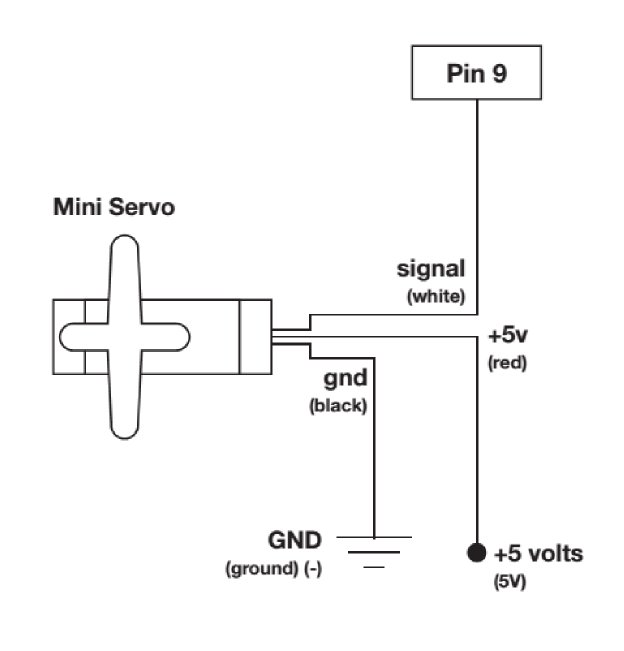
\includegraphics[scale=0.4]{servoCircuit.png}
\caption{Conexión de un ServoMotor.\label{circuitServo}}
\end{figure}

\item Cargue el programa mostrado anteriormente y verifique su funcionamiento.

\item Realice las modificaciones necesarias, para hacer que el servomotor se mueva a partir del ángulo de un potenciómetro. Una instrucción útil para esto:
	\begin{itemize}
		\item \texttt{map(input, minIn, maxIn, minOut, maxOut);}\\
		Retorna un entero que permite escalar la variable \texttt{input} que oscila entre los valores [\texttt{minIn}, {\tt maxIn}], entregando un resultado que oscila entre [{\tt minOut}, {\tt maxOut}]. 
	\end{itemize}	
\end{enumerate}

\section{Motores DC}

\begin{figure}[h]
\centering
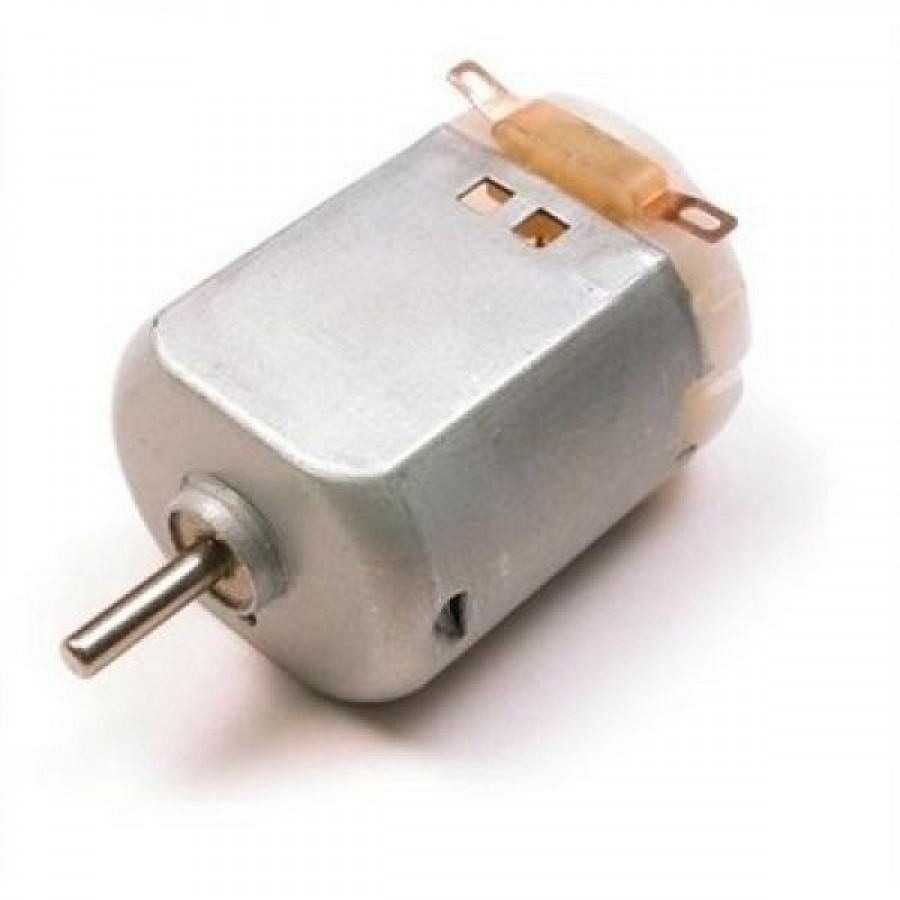
\includegraphics[scale=0.1]{motorDC.jpg}
\caption{Motor DC de escobillas.\label{motorDC}}
\end{figure}

Los motores DC --de corriente continua--, que podemos encontrar en juguetes y ventiladores de cpu, como el de la figura \ref{motorDC}, se caracterizan por girar inmediatamente después de conectarles una fuente de alimentación. Generalmente pueden funcionar a partir de los 3 volts, pero por lo menos requieren sobre 100mA de corriente para funcionar, corriente que lamentablemente no puede ser entregada por ninguna de las salidas de nuestra Arduino.\footnote{Atmel, recomienda un máximo de 20ma por salida para aplicaciones de prueba, en general se debe diseñar para que salga la minima corriente posible del microcontrolador.} Aquí enfrentamos un problema típico de la electrónica, que tiene que ver a grandes rasgos, con un área llamada \emph{Control de Potencia}, que se encarga de  \emph{acoplar} \textbf{señales de control} como las que trabaja Arduino, con \textbf{corrientes de fuerza} cómo la que necesita un motor para poder mover alguna carga o su propio eje.

Nace entonces, la necesidad de contar con la circuitería necesaria para realizar el \emph{acople} mencionado, generalmente este tipo de circuitos se conoce como \emph{Driver}.

A continuación, en la figura \ref{driverDC}, se muestra un driver básico hecho en base a un transistor 2n2222 que permite a Arduino manejar las corrientes que requiere el motor.

\begin{figure}[h]
\centering
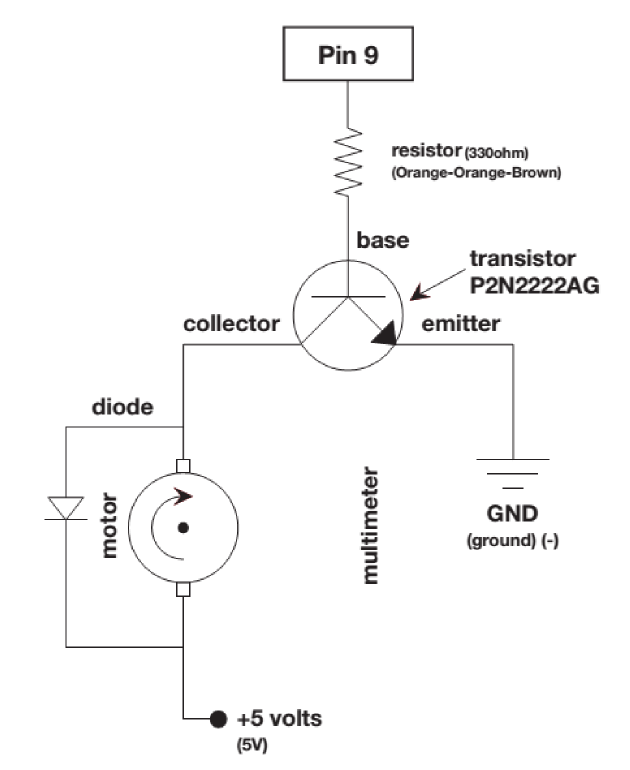
\includegraphics[scale=0.5]{driverDC.png}
\caption{Driver para motor DC basado en Transistor 2n2222.\label{driverDC}}
\end{figure}

Cabe notar que en este circuito, se utilizan dos elementos desconocidos hasta ahora, los cuales se describen brevemente a continuación:

\begin{itemize}
	\item {\bf Transistor:} Elemento semiconductor, que a partir de una pequeña corriente en su terminal de base, puede manejar proporcionalmente corrientes entre sus terminales Colector y Emisor. 		
	El modelo 2n2222 se caracteriza por poder manejar una corriente de hasta 200ma, lo que que resulta suficiente para nuestra aplicación.
	
	\item {\bf Diodo:} Elemento que permite el paso de la corriente en un solo sentido, en esta aplicación permite 
	bloquear corrientes producidas por el \emph{chisporroteo} del motor que, de no estar el diodo, terminarían dañando el transistor.
\end{itemize}

\subsection{Actividad}

\begin{enumerate}
\item Realice el montaje del circuito mostrado en la figura \ref{driverDC}. Con el fin de simplificar el montaje, se muestra de forma explícita la conexión en la figura \ref{driverDCdum}.

\begin{figure}[h]
\centering
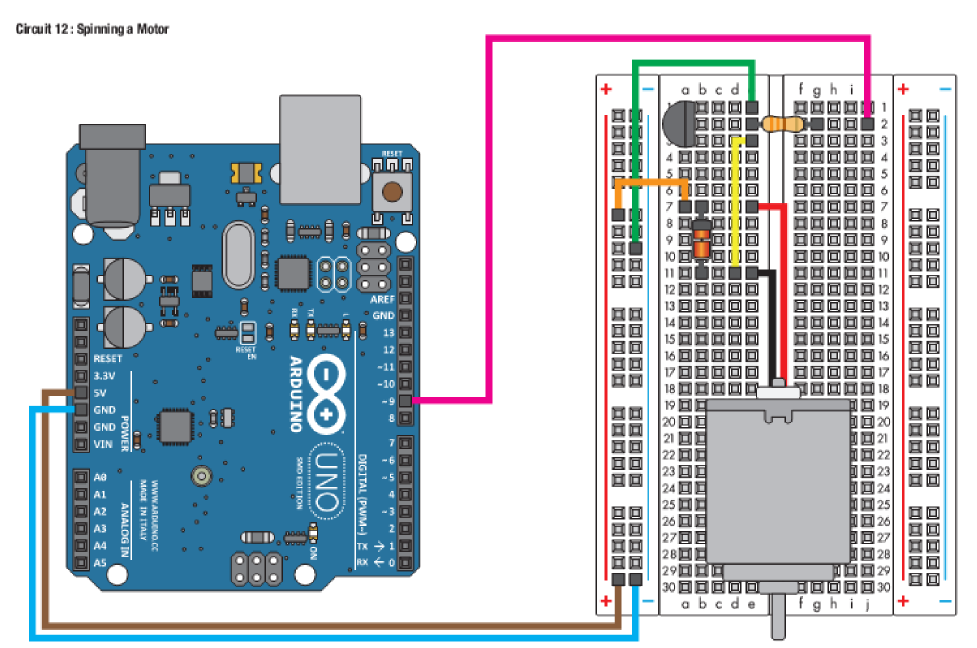
\includegraphics[scale=0.5]{driverDCdum.png}
\caption{Driver para motor DC, tomado de \cite{SIK}. \label{driverDCdum}}
\end{figure}

\item Escriba un programa --o reutilice alguno anterior--, que haga girar el motor durante un segundo, luego que este se detenga durante un segundo y que esto se repita eternamente.

\item Escriba un programa que envíe distintas señales PWM al pin 9, comente acerca del funcionamiento que presenta el motor. (Revise la sección \ref{pwmSec})
\end{enumerate}

\section{Cargas Fuertes y Corriente Alterna por medio de Relé}

En ocasiones, puede ser necesario utilizar Arduino para comandar artefactos cotidianos, cómo encender una ampolleta de nuestra casa, lo cual no sería posible, puesto que nuestra tarjeta trabaja con 5 volts en corriente continua y en nuestra vivienda el estándar es 220 volts en corriente alterna, por lo que cualquier interconexión directa entre ambos terminaría \emph{friendo} nuestra Arduino.

Bien se podría utilizar un transistor, pero no serviría el pequeño 2n2222 que utilizamos en prácticas anteriores, si no que en este caso, se requeriría calcular un driver que utilice arreglos de varios transistores con especificaciones para mayor potencia, los que en la actualidad son bastante caros y se utilizan mayormente en aplicaciones industriales como parte de costosos equipos, por lo cual descartamos este tipo de dispositivos para aplicaciones simples. Utilzaremos en cambio, un dispostivo bastante simple, llamado Relé.

\begin{figure}[h]
\centering
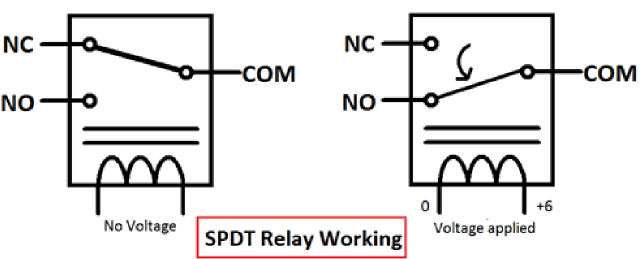
\includegraphics[scale=0.5]{relayDiag.png}
\caption{Diagrama simplificado de un Relé. \label{rele}}
\end{figure}

Un Relé, como el e la figura \ref{rele}, es un dispositivo que permite accionar magnéticamente un interruptor interno, en donde la principal característica es que tanto la bobina que produce el campo magnético como el interruptor, pueden pertenecer a circuitos distintos, es decir, podríamos accionar la bobina del dispositivo como si se tratara del motor DC de nuestro ejemplo anterior y el interruptor utilizarlo para accionar una ampolleta de nuestra casa. Lo anterior, además otorgar una \emph{Aislación Galvanica} entre nuestra Arduino y la red de 220VAC, es decir, no existe un camino eléctrico conductor entre ambas partes del circuito.

\begin{figure}[h]
\centering
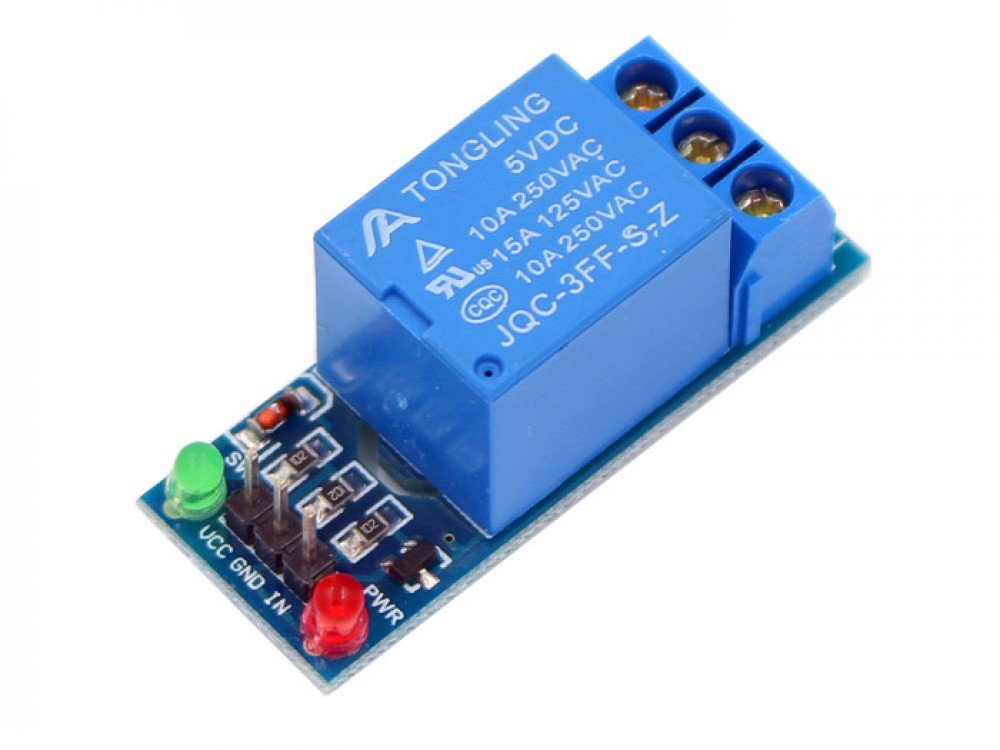
\includegraphics[scale=0.15]{relayModule.JPG}
\caption{Modulo Relé Integrado. \label{moduloRele}}
\end{figure}

En la figura \ref{moduloRele}, se muestra un Módulo Relé integrado, que permite manipular cargas de 220VAC directamente desde algún pin de nuestra Arduino.

\subsection{Actividad}

\begin{enumerate}
	\item Realice la conexión del sensor Ping (véase la sección \ref{pingSec}) y la conexión del Módulo Relé a los pines que usted estime conveniente. Para la parte de potencia del circuito, puede utilizar como guía la siguiente imagen. 
	
\begin{figure}[h]
\centering
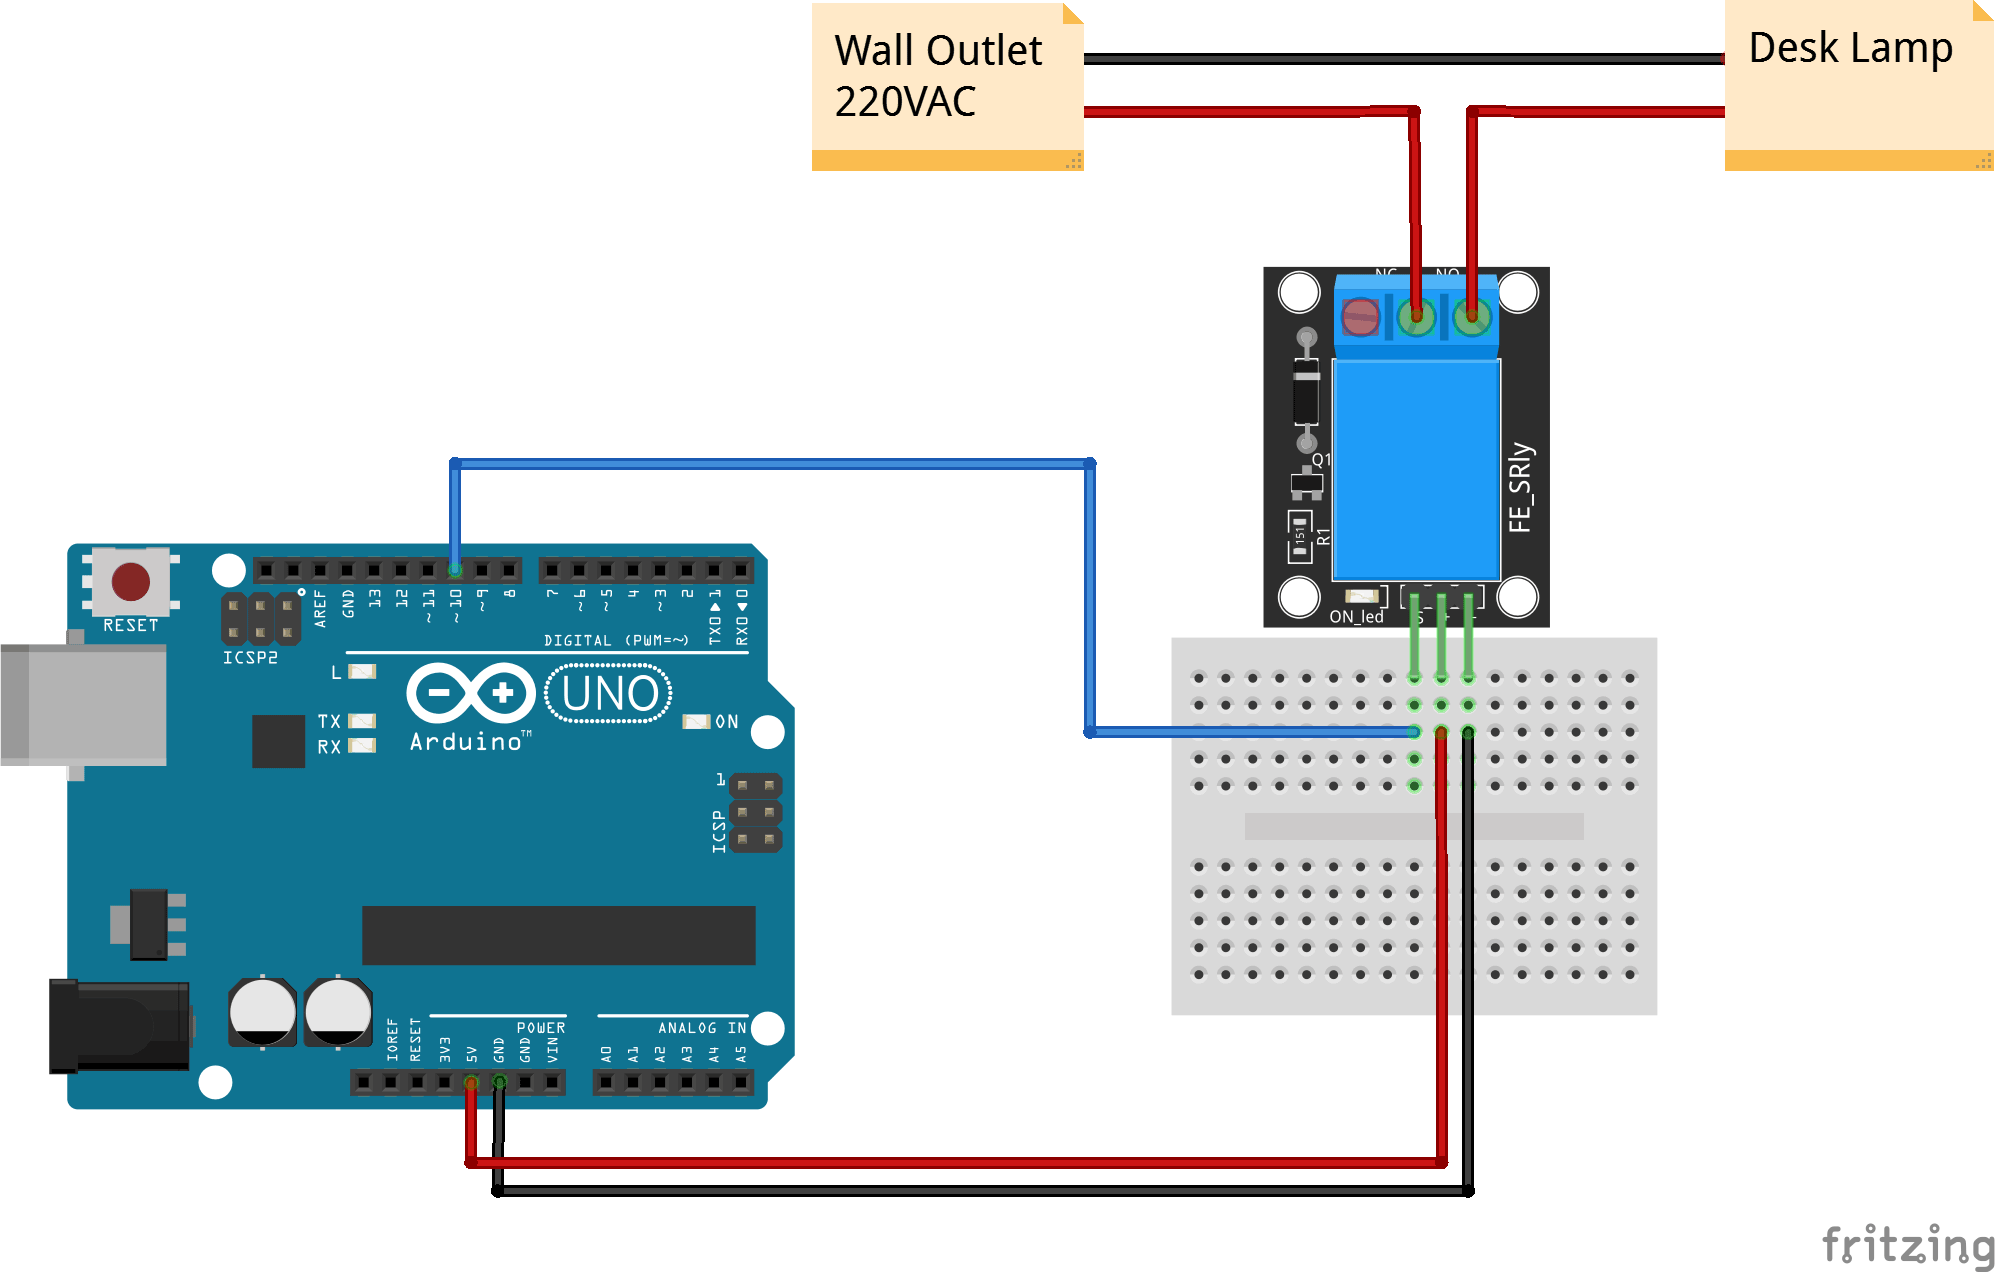
\includegraphics[scale=0.15]{relay.png}
\caption{Circuito con Relé y carga de 220VAC. \label{rele}}
\end{figure}


\item {\bf Smart-Home:} Desarrolle un programa, de manera que la luz se encienda, en cuanto alguien se acerque a menos de 1 metro del sensor ultrasónico y que esta permanezca encendido durante 5 segundos.

\begin{figure}[h]
\centering
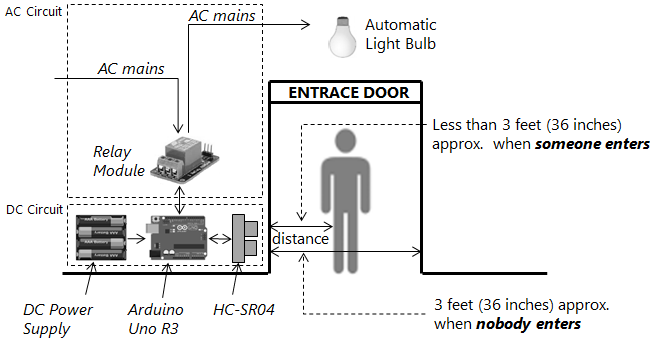
\includegraphics[scale=0.6]{aplicacion.png}
\caption{Ejemplo de Aplicación Smart-Home.}
\end{figure}

\end{enumerate}

\chapter{Introducción a los Sistemas de Control Automático}

\section{Automatización}
En general, cuando se habla de \emph{Automatización} inmediatamente se asocia el concepto a sistemas inteligentes, sistemas que realizan tareas repetida e incansablemente o sistemas que controlan alguna variable de interés, como por ejemplo puertas de recintos comerciales que se abren cuando algún cliente se acerca a ellas, rápidas lineas de ensamblaje que completan varias tareas al minuto o un climatizador que mantiene la temperatura que el usuario quiera independiente de las condiciones ambientales exteriores; son todos sistemas automáticos que en cierta medida no requieren la intervención de un ser humano para su pleno funcionamiento.
\vspace{10pt}

\textbf{Automático}
\begin{quotation}
	\it
	Que funciona por sí solo o que realiza total o parcialmente un proceso sin ayuda humana.
\end{quotation}
\vspace{10pt}
Es posible diferenciar dos tipos de sistemas que tienen propósitos diferentes pero no dejan de ser automáticos. Por ejemplo 
\begin{itemize}
	\item Se tiene un estanque con dos botones que al ser presionados comanda el vaciado o llenado completo del recipiente.
	\begin{figure}[h]
		\centering
		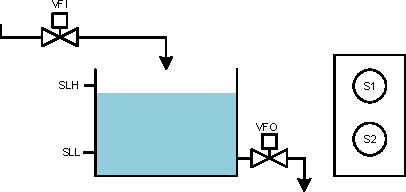
\includegraphics[scale=0.8]{Estanque.pdf}
		\caption{Estanque de Control Discreto del Nivel.}	
	\end{figure}
	
	\item Se tiene un sistema que controla el nivel del estanque que es capaz de purgar los excesos de nivel perdido mediante la apertura gradual de una válvula.
	\begin{figure}[h]
		\centering
		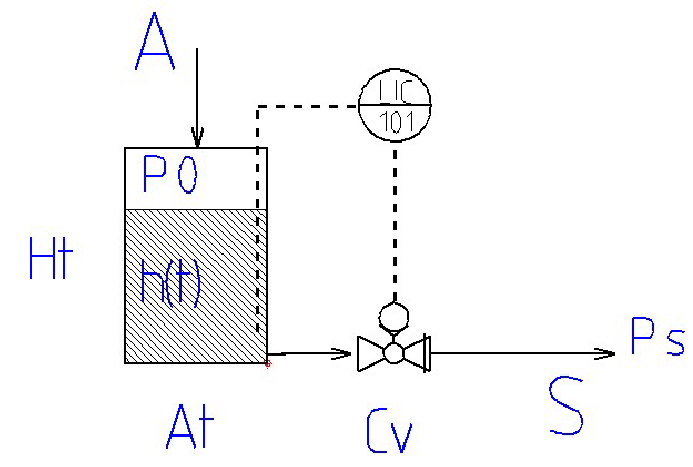
\includegraphics[scale=0.23]{EstanqueControl.png}
		\caption{Diagrama P\& ID del Control Continuo del Nivel de Estanque}	
	\end{figure}

\end{itemize}	
	La diferencia fundamental entre estos dos sistemas, es que uno automatiza una \emph{tarea} mientras que el otro realiza una \emph{regulación} automática permanente en el tiempo.
	
	\section{Control de Eventos Discretos}
	Es la automatización de tareas repetitivas y eventos discretos que no requieren mayor inteligencia, por lo que pueden ser ejecutados por maquinas de forma reiterativa y a gran velocidad. Se dividen en tareas y eventos que tienen un comienzo y un final. Dentro de este tipo de sistemas se encuentran.
	\begin{itemize}
		\item Partidas directas e inversores de giro con elementos de comando eléctrico.
		\item Encender o apagar las luces de una vivienda a horarios determinados.
		\item Encender o apagar las luminarias en la vía pública cuando se ha escondido el sol.
		\item Ensamblar piezas mediante brazos robóticos.
	\end{itemize}	
	
	\section{Control Regulatorio}
	
	Consiste en mantener variables físicas en un valor deseado según estrategias acuñadas por la \emph{Teoría de Control} que generalmente requieren un análisis matemático avanzado de la física que involucra el proceso que se quiere controlar.
	
	En su forma más básica, el control regulatorio se logra siguiendo la \emph{Estructura General de Control} detallada a continuación.
	
	\section{Estructura general de control}
	Al representar las distintas partes del sistema como bloques las partes necesarias para controlar una variable junto con las interconexiones entre las mismas son las siguientes. 
	
	\begin{figure}[h]
		\centering
		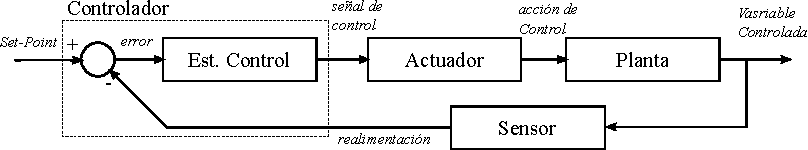
\includegraphics[scale=0.9]{egControl.pdf}
		\caption{Estructura General de un Sistema de Control.\label{egControl}}	
	\end{figure}

	\subsection{Bloques del Sistema}	
	
	\begin{itemize}
	\item {\bf Controlador: }
	Es un equipo al que se ingresa el valor de set point, se conecta el sensor y el actuador. Contiene la Estrategía de Control y en base a esta comanda al actuador según la magnitud de la diferencia entre el valor deseado y el valor actual que mide el sensor.
	
	\item {\bf Actuador: }
	Es el encargado de ejercer la  \emph{Acción de Control}, es comandado por el controlador y es el que provee el esfuerzo necesario para cambiar el estado actual de la variable de salida del proceso. Se conoce tambien con el nombre de \emph{Elemento Final de Control}.
	
	\item {\bf Proceso: }
	Comunmente se le llama \emph{Planta}, y es el proceso físico que se quiere controlar, por ejemlo un estanque con su dinámica de llenado y vaciado, una caldera con toda la física involucrada en el calentamiento del agua y su transformación a vapor. Este bloque, recibe la acción de control cambiando su estado, siendo este medido por el sensor e informando al controlador.
	
	\item {\bf Sensor: }
	Se encarga de informar al controlador acerca del estado actual del proceso que se quiere controlar, es el encargado de producir la \emph{Realimentación} necesaria para que el sistema sea controlado.
	\end{itemize}
	
	\subsection{Señales del Sistema}
	
	Son las líneas que interconectan cada uno de los bloques.
	\begin{itemize}
	\item {\bf Set-Point SP: }
 Es el valor deseado para el sistema en cuestión, tiene la misma magnitud que la variable de salida, por ejemplo si se controla el nivel de un estanque, el set point, será un nivel determinado, por ejemplo 5m de altura. También se conoce con los nombres de \emph{Señal de Consigna}, \emph{Señal de Referencia}, \emph{Entrada del Sistema}, entre otros.
	
	\item {\bf Error: }
 Es el valor resultante de la resta del Set-point con el Valor actual del proceso informado por realimentación que provee el sensor. Cuando este valor es cero se dice que el sistema esta controlado.
	
	\item {\bf Señal de Control MV: }
 Es la señal de comando para el actuador  generada en el controlador de acuerdo al error calculado según lo que dicte la estrategia de control.
	
	\item {\bf Acción de Control: }
 Es el esfuerzo físico que ejerce el actuador, puede ser cerrar una válvula, encender un calefactor, encender un ventilador, etc.
 
	
	\item {\bf Realimentación PV:} Es la señal eléctrica enviada por el sensor para informar al controlador el estado actual de la planta.
\end{itemize}

\section{Aplicación de Arduino cómo Sistema de Control Regulatorio}

A continuación, se presenta un sistema de control de un proceso físico, en donde Arduino actúa como controlador. El sistema consiste en la levitación de una bolita de poliestireno a una altura deseada, por medio del empuje de una corriente de aire producida por un ventilador de CPU; la altura es sensada de forma continua por un sensor ultrasónico Ping y el Set-Point se modifica mediante un potenciómetro conectado al Arduino. En la figura \ref{levitron1}, se muestra un esquema del sistema. 

\begin{figure}[h]
	\centering
	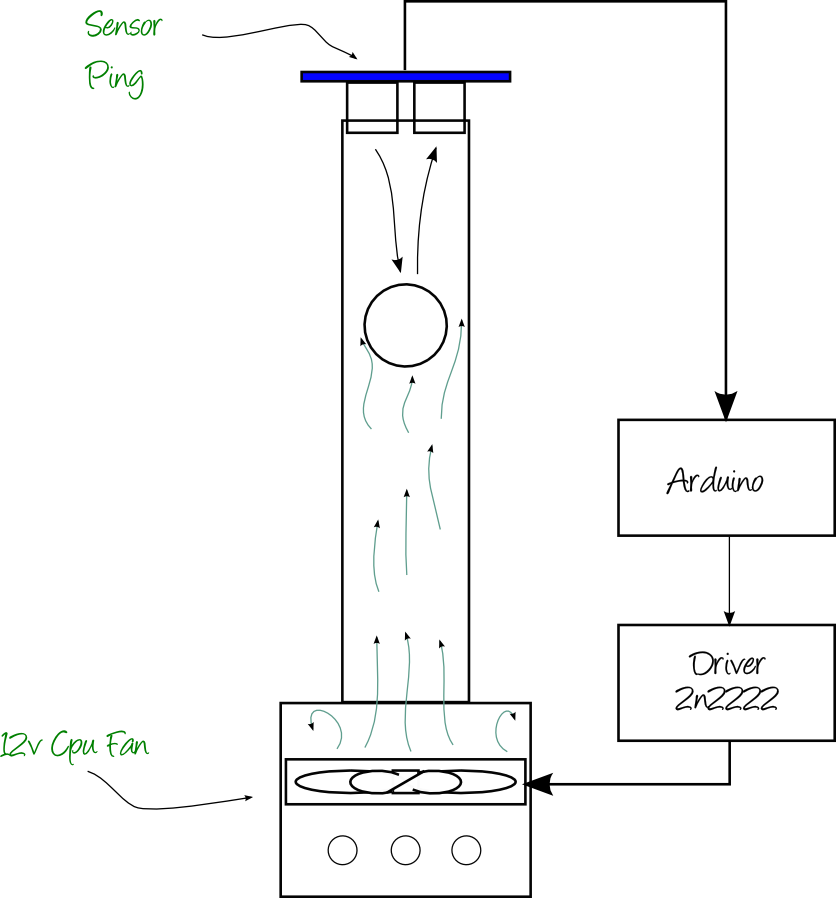
\includegraphics[scale=0.4]{levitron.png}
	\caption{Sistema de control de levitación por aire. \label{levitron1}}
\end{figure}	

A grandes rasgos, el sistema permite manipular la altura a la que levita la bolita, mediante un potenciómetro. Si analizamos el sistema mediante la \emph{Estructura General de Control} de la figura \ref{egControl}, tenemos el caso mostrado a continuación. (figura \ref{controlLevi})

\begin{figure}[h]
	\centering
	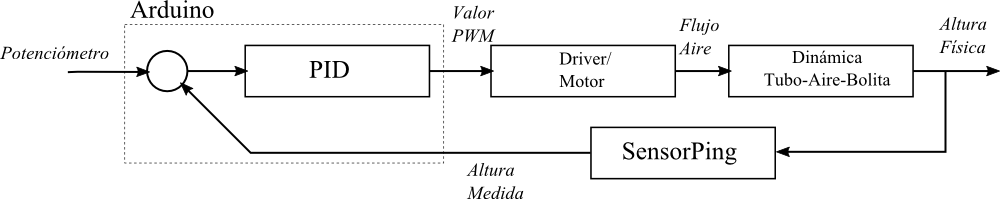
\includegraphics[scale=1]{controlLevi.png}
	\caption{Estructura general de control aplicada al sistema. \label{controlLevi}}
\end{figure}

Cabe notar, que en el bloque correspondiente a la \emph{Estrategia de Control}, encontramos las siglas PID, puesto que es precisamente el nombre de la estrategia que se utilizará para calcular la potencia que se debe enviar al actuador para obtener una altura determinada.

\subsection{Control Proporcional Integral y Derivativo PID}

Es una estrategia de control, que permite calcular la magnitud de la \emph{Acción de Control} para que el valor de la \emph{Realimentación} se iguale al valor del \emph{Set-Point} y que que aunque el cálculo no lleve a un buen resultado, el sistema por sus característica iterativa logrará llegar al punto buscado.

El control PID se basa en tres constantes, llamadas \textbf{Proporcional, Integral} y \textbf{Derivativa}, las cuales son ponderaciones que se otorgan al valor de la acción de control en base al \emph{Error}, es decir, podemos tener un sistema sensible a los tres siguiente parámetros:

\begin{itemize}
	\item \textbf{Constante Proporcional: } permite ajustar la sensibilidad del sistema al tamaño del error, es decir, mientras mayor sea el error, mayor será la acción que se ejerza sobre el sistema.
	
	\item \textbf{Constante Proporcional: } permite ajustar la sensibilidad del sistema al tiempo que este aguantará que se presente el error, es decir, a mayor constante integral, el sistema tolerará durante menos tiempo un error estático aumentando el valor de la acción de control en el tiempo.
	
	\item \textbf{Constante Proporcional: } ajusta la sensibilidad del sistema a la tasa de cambio del error, es decir, si el sistema se acerca o se aleja muy rápido del Set-Point, la acción de control aumentará o disminuirá acorde a esa velocidad.
\end{itemize}

\subsection{Codigo que Implementa el Control del Sistema}

 A continuación, se presenta el código que permite controlar la levitación de la bolita de poliestireno.
 
 \begin{lstlisting}[style=myArduino]
 #include <PID_v1.h>

const int pingPin = 7;            //Ultrasonic sensor Pin
const int fanPin  = 8;            //Actuator Pin (fan)
const int potPin  = 5;            //Potentiometer to set the Sp

double Sp, Pv, Mv;                //Values for PID control

//Compensator Values
double kp = 5;                    //Proportional
double ki = 3;                    //Integral
double kd = 3;                    //Derivative

//Compensator declaration
PID myPID(&Pv, &Mv, &Sp, kp, ki, kd, REVERSE);

void setup() {
  
  Serial.begin(9600);
  
  Pv = 29;                  //initial PV Value to trigger the actuator.
  Sp = 18;                  //initial SetPoint
  
  myPID.SetMode(AUTOMATIC);
  myPID.SetOutputLimits(0,255);

}

void loop() {
  
  Sp = map(analogRead(potPin),0,1023,3,29);
  Pv = usonicMeas();
  
  myPID.Compute();
  
  analogWrite(fanPin,Mv);

  showVariables();          //list Sp,Pv and Mv on Serial Monitor
  
}

long usonicMeas(){

  //shape the pulse
  
  pinMode(pingPin, OUTPUT);
  digitalWrite(pingPin, LOW);             
  delayMicroseconds(2);         
  digitalWrite(pingPin, HIGH);  
  delayMicroseconds(5);
  digitalWrite(pingPin, LOW);

  //Measure Time of Flight
  
  pinMode(pingPin, INPUT);                //act as input
  long duration = pulseIn(pingPin, HIGH); //Read the pulse
  return duration / 29 / 2;               //return value in centimeters
  
}

void showVariables(){
  
  Serial.print(Sp);
  Serial.print(", ");
  Serial.print(Pv);
  Serial.print(", ");
  Serial.println(Mv);  

}
 
 \end{lstlisting}

\subsection{Actividad}

En base a la explicación del código anterior, provista por el profesor, realice las siguientes tareas:

\begin{enumerate}
	\item Identifique a partir del código y la información presentada, el diagrama de conexiones que requiere este circuito, indicando claramente los pines del Arduino donde deben ir conectados los elementos:
	\begin{itemize}
		\item Sensor Ping.
		\item Cpu Fan y driver 2n2222.
		\item Potenciometro.
	\end{itemize}
	
	\item Identifique la sección de código que se encarga de la medición de la altura de la bolita y como funciona esta.
	
	\item Explique que función cumple la instrucción \texttt{analogRead} dentro de todo el sistema de control.
\end{enumerate} 

%%%%%%%%%%%%%%%%%%%%%%%%%%%%%%%%%%%%%%%%%%%%%%%%%%%%%%%%%%%%%%%%%%%%%%%%%%%%%%%%%%%%%%%%%%%%%%%%%%%%%%%%5555

\chapter{Internet de las Cosas con Raspberry Pi}

\begin{center}

\includegraphics[scale=0.15]{logoRaspberry.png}
\end{center}

Raspberry Pi es un pequeño computador del tamañano de una tarjeta de crédito, el cual podemos conectar fácilmente a una televisión vía HDMI o RCA como salida de video. Además al ser un computador, podemos utilizarla, con un teclado y un mouse. Tiene conexión vía Ethernet, bus USB y pines GPIO (General Purpose Input/Output), para que podamos interactuar con nuestra placa con sensores, botones, entre otros. Pese a que el sistema operativo que se utiliza por defecto como parte del proyecto; {\bf Raspbian}, tiene capacidades de reproducción de vídeo en alta definición, procesadores de texto tipo \emph{Office} y juegos tipo \emph{Arcade}, realmente la mayor utilidad de este sistema computacional, se encuentra en el desarrollo de sistemas computacionales embebidos, es decir, aquellas aplicaciones que requieran de procesamiento de datos, cómo \emph{Data-Mining}, visión artificial, recolección de Big-Data, entre otros y que no necesiten de un entorno gráfico o siquiera un escritorio, pues el hardware se halla inserto en algún proceso o sistema muy lejos de parecerse el escritorio de una oficina con teclado, mouse y pantalla.

\section{Primer Encendido y Configuración Para Uso Remoto}

\begin{figure}[h]
\centering
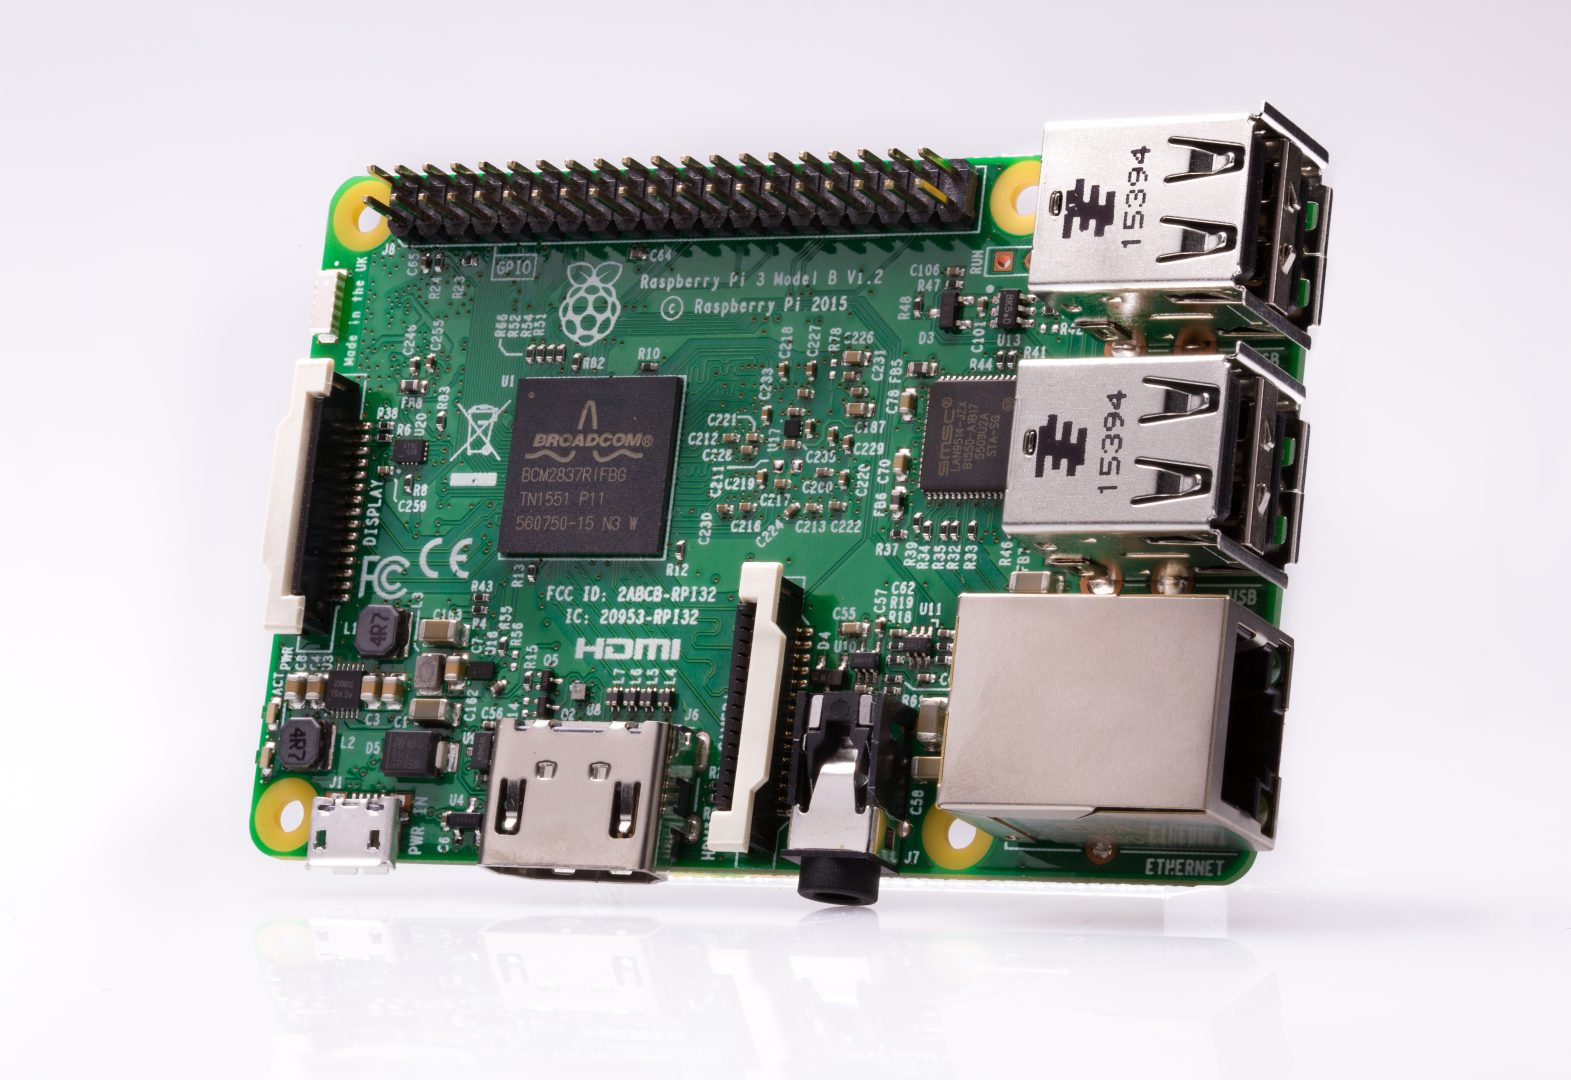
\includegraphics[scale=0.25]{pi3.jpg}
\caption{Raspberry Pi 3 Model B.\label{RPI}}
\end{figure}

Este curso, considera el uso de la variante de Raspberry Pi 3, precargada con el sistema operativo Raspbian, entre las especificaciones computacionales de esta tarjeta se destaca:
\begin{itemize}
\itemsep=0pt
	\item Quad Core 1.2GHz Broadcom BCM2837 64bit CPU.
	\item 1GB RAM.
	\item Conectivididad wireless LAN y Bluetooth de bajo consumo energético.
	\item 40 pines GPIO.
	\item 4 puertos USB 2.0.
\end{itemize}

Nuestro primer encendido, lo haremos como si se tratase de un computador de escritorio, por lo tanto necesitamos contar con un \textbf{Teclado, un Mouse y una Pantalla}, además de una \textbf{tarjeta SD previamente cargada con el sistema operativo Raspbian} y respectiva alimentación de 5 volts, capaz de proveer 2.5A. Con ello, podremos a punto nuestra Raspberry para poder deshacernos de todo el aparataje que conllevan los periféricos nombrados, pudiendo acceder desde la comodidad de nuestro computador portatil por medio de una conexión de \textbf{Escritorio Remoto VNC} o \textbf{SSH} en caso de no ser necesario un entorno gráfico. 

\subsection{Actividad: Configuración de Raspberry para conexión remota}

\begin{enumerate}
	\item Conectamos Teclado, Mouse, Monitor, Tarjeta SD y Alimentación a nuestra Raspberry.  Aquí deberíamos ver un encendido típico de una maquina Linux, primero iniciando y luego detenerse en el escritorio clásico de Gnome. (figura \ref{startup})

\begin{figure}[h]
	\centering
	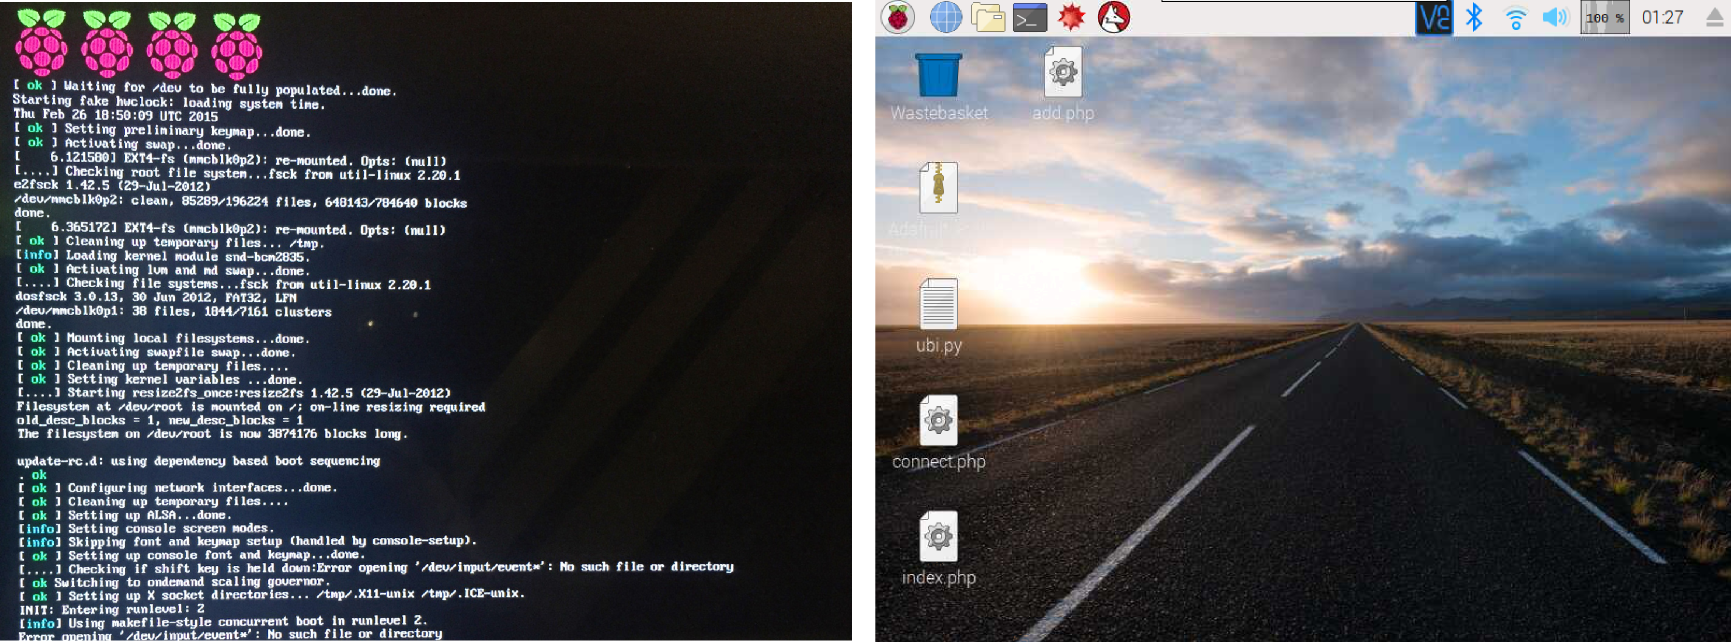
\includegraphics[scale=0.3]{startup.png}
	\caption{Pantallas de inicio al encender Raspberry Pi. \label{startup}}
\end{figure}	

\item Con el fin de habilitar el acceso remoto a nuestra Rpi, vamos al \emph{Applications Menu>Preferences>Raspberry Pi Configuration}, una vez abierta la ventana correpondiente, seleccionamos la pestaña \emph{Interfaces} y marcamos las opciones que nos interesen. Con fines de desarrollo, es común habilitarlas todas. (figura \ref{piConf})

\begin{figure}[h]
	\centering
	\includegraphics[scale=0.3]{piConf.png}
	\caption{Configuración de interfaces de Raspberry. \label{piConf}}
\end{figure}

\item Instalamos el software que nos permitirá acceder de manera gráfica nuestro escritorio \textbf{Real VNC Server} mediante el clásico terminal de linux y el comando Apt.

\begin{center}
	\texttt{sudo apt-get install realvnc-vnc-server}
\end{center} 

Curiosamente, esta distro de linux, no pide contraseña de administrador al ejecutar el comando \texttt{sudo}. De todas maneras, el usuario del escritorio es \texttt{Pi} y la contraseña de este es \texttt{raspberry}, y en caso del usuario \texttt{root}, la contraseña es la misma. 

\item Conectamos nuestra Rpi a la red. Ya sea por medio de WiFi o de manera cableada y registramos la IP que nos ha asignado el Router, para poder acceder con ella nuestro escritorio remoto.

En el terminal ingresamos \texttt{sudo ifconfig}, ante lo cual nos debería aparecer una respuesta del tipo mostrado en la figura \ref{ifconfig}. Mientras no desconectemos nuestra Raspberry, podremos acceder mediante esta IP desde nuestro PC o portátil. En caso de deconectarnos, aun existen muchas maneras de descubrir o incluso fijar la IP de nuestra Raspberry, ello escapa a los contenidos de este curso, pero un buen manejo técnico de redes de datos siempre podrá resolverlo. 

\begin{figure}[h!]
	\centering
	\includegraphics[scale=0.6]{ifconfig.png}
	\caption{Respuesta del comando \texttt{sudo ifconfig}. \label{ifconfig}}
\end{figure}


\item Finalmente, desde nuestro portátil o PC podremos ingresar de manera remota a nuestra Rpi con la IP, usuario y contraseña correspondientes, desde el software RealVNC, tal como se muestra en la imagen \ref{vnc}.

\begin{figure}[h!]
	\centering
	\includegraphics[scale=0.3]{vnc.png}
	\caption{Conexión VNC con Raspberry desde Windows 7. \label{vnc}}
\end{figure}
\end{enumerate}

\newpage
\section{Control de GPIO's en Python}

Como ya se vio antes, en la introducción de este curso, los GPIO's son pines de entradas o salidas de propósito general, en términos simples, son pines digitales como los de Arduino que pueden ser programados por medio de lenguajes de alto nivel como \textbf{Python}.

Dependiendo del modelo de Raspberry a utilizar, puede que este traiga o no escritos los nombres de sus respectivos pines, como por ejemplo, el caso de Pi Zero que no trae nombre en sus pines. De todas formas los modelos siguen el mismo \emph{Pinout} con pequeñas variaciones, por ejemplo en la figura \ref{gpios} se muestra el correspondiente al modelo B+.
\begin{figure}[h!]
	\centering
	\includegraphics[scale=0.55]{gpios.png}
	\caption{Enumeración de GPIO's de Raspberry Pi modelo B+. (tomada de \cite{gpio}) \label{gpios}}
\end{figure}

\textbf{Nota:} La mayoria de los GPIO's tienen conexión directa con el chip Broadcom, por lo tanto al lidiar con circuitos conectados a estos pines, existe un gran riesgo de inhabilitar nuestra Raspberry.

\subsection{Actividad: Manejo de GPIO's desde Python}
\begin{enumerate}
	\item Preparar el circuito a utilizar durante todo este capítulo, para ello realizar el montaje mostrado en figura \ref{testPi}.
	
	\begin{figure}[h!]
	\centering
	\includegraphics[scale=0.8]{testPi.png}
	\caption{Circuito de prueba para control de GPIO's desde Python. \label{testPi}}
\end{figure}
	
	\item Instalar o revisar la instalación del interprete de Python 3 y el módulo Rpi.GPIO mediante el siguiente comando desde una terminal.
	
	\begin{center}
	\texttt{sudo apt-get install python-dev python-rpi.gpio}
	\end{center}
	
	Lo anterior, procederá a instalar lo mencionado, o en su defecto, nos permitirá verificar una instalación previa.
	
	\item Por medio de un Terminal, creamos un archivo para nuestro código, con el comando:\\
	\begin{center}	
	\texttt{nano blink.py}
	\end{center}
	
	Luego, en el editor de texto, escribimos el siguiente código:
	
	\begin{lstlisting}[language=Python, style=myArduino]
import RPi.GPIO as GPIO
import time
GPIO.setmode(GPIO.BCM)
GPIO.setup(17, GPIO.OUT) ## GPIO 17 como salida
GPIO.setup(27, GPIO.OUT) ## GPIO 27 como salida

def blink():
        print "Comienzo Programa..."
        while 1:
                GPIO.output(17, True) 	## Enciendo el 17
                GPIO.output(27, False) 	## Apago el 27
                time.sleep(1) 			## Esperamos 1 segundo
                GPIO.output(17, False) 	## Apago el 17
                GPIO.output(27, True) 	## Enciendo el 27
                time.sleep(1) 			## Esperamos 1 segundo
        GPIO.cleanup() ## Hago una limpieza de los GPIO	
        
blink()	##llamamos a la funcion
\end{lstlisting}	

Una vez escrito el código, presionamos CTRL+X y aceptamos guardar los cambios.

\item Finalmente, ejecutamos nuestro código con permisos de administrador, mediante la siguiente instrucción:
\begin{center}
	\texttt{sudo python blink.py}
\end{center}

Si todo ha resultado bien, hasta esta parte deberiamos ver en el terminal el mensaje \texttt{Comienzo Programa...} y nuestros leds deberían comenzar a parpadear según los tiempos programados.

\item Finalmente, modifique los tiempos de encendido de los Led y verifique el funcionamiento de la implementación.
\end{enumerate}

\newpage
\section{Servicio IoT Ubidots.com}

\begin{center}
\includegraphics[scale=0.3]{ubidots.png}
\end{center}

Ubidots.com es un servicio para aplicaciones de \emph{Internet de las Cosas} IoT, que existe desde 2014, presta servicios comerciales de almacenamiento de datos en la nube y posee un muy buen soporte, independiente si se trata de cuentas de pago o educacionales, además de contar con una creciente comunidad que genera material para la mayoría de las plataformas hardware y software actuales, como Raspberry Pi, Arduino, NodeMCU, entre otras.

Su funcionamiento es bastante simple. Se basa en cuentas de usuario, aseguradas por un \emph{Token}\footnote{Identificador único para cada cuenta}, en donde uno pude crear dispositivos, los que a su vez pueden contener variables con identificadores únicos, las cuales, contienen el historial de datos datos almacenados que bien podrían ser enviados por elementos tanto físicos como elementos software. Una vez, puestas a punto, las variables y dispositivos, se pueden crear vistosos \emph{Dashboards} que permiten tanto visualizar como manipular los datos contenidos en las variables. (figura \ref{dashboard})

\begin{figure}[h!]
	\centering
	\includegraphics[scale=0.2]{dashboard.jpg}
	\caption{Ejemplo de Dashboard en Ubidots. \label{dashboard}}
\end{figure}

Ubidots cuenta con API's y librerías, que permiten tanto subir como bajar datos, desde todo tipo de aplicaciones, incluyendo un módulo para Python.

\subsection{Actividad: Cuenta y Dispositivos en Ubidots}

\begin{enumerate}
\item Diríjase al sitio \texttt{ubidots.com} y en el botón \emph{Signup}, complete la información requerida y siga los pasos para crear una cuenta, necesitará de una dirección de correo electrónico.

\item En la parte superior de su cuenta, en \emph{Devices}, cree un nuevo dispositivo y llámelo \emph{Raspberry} o el nombre que usted prefiera, a su vez, dentro del dispositivo cree las variables \texttt{cuenta}, \texttt{led1} y \texttt{led2}. Debería ver pantallas como las que se muestran en la figura \ref{dispo}.

\begin{figure}[h!]
	\centering
	\includegraphics[scale=0.3]{dispositivo.png}
	\caption{Creación de un dispositivo y variables. \label{dispo}}
\end{figure}

\item Finalmente, tome nota de su \emph{Token} y sus \emph{Variable ID's}, cómo se muestra en la figura \ref{varid}. Se recomienda seguir las instrucciones del relator.

\begin{figure}[h!]
	\centering
	\includegraphics[scale=0.6]{varid.png}
	\caption{Identificador de variable. \label{varid}}
\end{figure}

\item En la parte superior de su cuenta, en \emph{Dashboard}, cree una pantalla escogiendo \emph{widgets} de manera que se muestre algo como lo mostrado en la figura \ref{dash}.

\begin{figure}[h!]
	\centering
	\includegraphics[scale=0.4]{dash.png}
	\caption{Dashboard con nuestras variables. \label{dash}}
\end{figure}

\end{enumerate}

\subsection{Actividad: Envío de datos a Ubidots}
A continuación, se presenta una implementación que genera una variable en un script en Python y envía dicha variable a una cuenta en Ubidots. Lo anterior, puede ser fácilmente modificado para el envío de datos tomados por algún sensor.

\begin{enumerate}
\item Primero, necesitamos instalar el módulo que permite que Python comunique con Ubidots. Para ello en un terminal ejecutamos:

\begin{verbatim}
$ sudo apt-get install python-setuptools
$ sudo easy_install pip
$ sudo pip install ubidots
\end{verbatim}



\item Manteniendo el circuito de la figura \ref{testPi}, de actividades anteriores, creamos un archivo llamado \texttt{contador.py} con el siguiente código:

\begin{lstlisting}[language=Python, style=myArduino]
import RPi.GPIO as GPIO
from ubidots import ApiClient
import time
GPIO.setmode(GPIO.BCM)
GPIO.setup(22, GPIO.IN)
GPIO.setup(17, GPIO.OUT)

api = ApiClient(token='SU-TOKEN')
contador = api.get_variable('ID-VARIABLE-CONTADOR')

def program():
        print "Ejecucion iniciada..."
        i = 0
        while 1:
                if GPIO.input(22):

                        while GPIO.input(22):
                                pass
                        i=i+1
                        print i
                        contador.save_value({"value": i})
        GPIO.cleanup()

program() ## Hago la llamada a la funcion
\end{lstlisting}

El código resulta bastante intuitivo. En síntesis, cada vez que se presiona el botón conectado a GPIO22 aumenta un valor de cuenta en una unidad y envía ese valor la variable \emph{Contador} de nuestra cuenta.

\item Finalmente, ejecute el código y verifique su funcionamiento; al presionar el boton conectado a la Raspberry el valor de cuenta, debería aumentar al mismo tiempo que lo hace en el Dashboard.
\end{enumerate}

\subsection{Actividad: Accionamiento de dispositivos desde Ubidots}

A continuación, se presenta una implementación, que permite accionar elementos discretos desde una cuenta en Ubidots. Lo anterior, mediante el uso de módulos relé puede perfectamente permitir la activación o desactivación de artefactos electrodomésticos desde la nube.

\begin{enumerate}
\item Manteniendo el circuito de la figura \ref{testPi}, de actividades anteriores, creamos un archivo llamado \texttt{leds.py} con el siguiente código:

\begin{lstlisting}[language=Python, style=myArduino]
import RPi.GPIO as GPIO
from ubidots import ApiClient
import time
GPIO.setmode(GPIO.BCM)
GPIO.setup(27, GPIO.OUT)
GPIO.setup(17, GPIO.OUT)

api = ApiClient(token='SU-TOKEN')
led2 = api.get_variable('VAR-ID-LED2')
led1 = api.get_variable('VAR-ID-LED1')

def program():
        print "Ejecucion iniciada..."

        while 1:
                valorLed1 = led1.get_values(1)
                valorLed2 = led2.get_values(1)

                print "led 1 " + str(valorLed1[0]['value'])+", led 2 "+ str(valorLed2[0]['value'])

                if valorLed1[0]['value']==1.0:
                        GPIO.output(17,True)
                else:
                        GPIO.output(17,False)

                if valorLed2[0]['value']==1.0:
                        GPIO.output(27,True)
                else:
                        GPIO.output(17,False)

                if valorLed2[0]['value']==1.0:
                        GPIO.output(27,True)
                else:
                        GPIO.output(27,False)
        GPIO.cleanup()

program() ## Hago la llamada a la funcion
\end{lstlisting}

En este caso, el código, se encarga de leer el valor de las variables \emph{Led1} y \emph{Led2} en nuestra cuenta de Ubidots y en base al valor que estos presenten, enciende o apaga los GPIOS 27 y 17.

\item Ejecute el código y verifique su funcionamiento. El terminal de linux debería permanecer mostrando los valores 0.0 ó 1.0 para los leds 1 y 2, mientras que al presionar los botones del dashboard mostrado en la figura \ref{dash}, los leds conectados a nuestra Raspberry deberían cambiar su estado.

\item Adicionalmente, puede descargar la aplicación \emph{Ubidots Explorer} para smartphones con sistema operativo Android y comandar su aplicación desde allí. Tal como se muestra en la figura \ref{android}.
\begin{figure}[h!]
	\centering
	\includegraphics[scale=0.2]{android.png}
	\caption{App Ubidots Explorer. \label{android}}
\end{figure}

\end{enumerate}


 
\begin{thebibliography}{9}

	\bibitem{libroMicro}
  		 Dogan Ibrahim, 
  		\textit{Programación de Microcontroladores Pic},
  		Editorial Marcomobo,
  		2007.
  		
  	\bibitem{atmegaDatasheet}
  		Hoja de Datos ATmega328p, \textit{8-bit AVR Microcontrollers ATmega328P
 		DATASHEET COMPLETE}\\
 		\verb@http://www.atmel.com/Images/@ \\
 		\verb@Atmel-42735-8-bit-AVR-Microcontroller-ATmega328-328P_Datasheet.pdf@
 		
 	\bibitem{queEsArduino}
 		Introducción a Arduino, \textit{What is Arduino?}\\
 		\verb@https://www.arduino.cc/en/Guide/Introduction@
 		
 	\bibitem{SIK}
 	Adafruit Industries, \textit{SparkFun Inventor’s Guide}\\
 	Guía ilustrada adjunta al kit de iniciacion en Arduino Sparkfun Inventors Kit.
 
 	\bibitem{Serial}
 	Serial -- Arduino Reference\\
 	\texttt{https://www.arduino.cc/reference/en/language/functions/communication/serial/}
 	
 	\bibitem{LM35}
 	Texas Instruments, {\it LM35 Temperature Sensor Datasheet}\\
 	\texttt{http://www.ti.com/lit/ds/symlink/lm35.pdf}
 	
 	\bibitem{guiaControl}
 	Antonio David Vásquez Briones, \emph{Conceptos de Automatización}\\
 	Apunte para asignatura Sistemas de Control Automático, Inacap Concepción.
 	
 	\bibitem{realVNC}
 	Sitio de Descargas de Real VNC para disintos SO's.\\
 	\texttt{https://www.realvnc.com/es/connect/download/vnc/}
 	
 	\bibitem{gpio}
 	Guía para GPIO's en Raspberry Pi. \\
 	\emph{Simple Guide to the RPi GPIO Header and Pins}\\
 	\texttt{https://www.raspberrypi-spy.co.uk/2012/06/simple-guide-to-the-rpi-gpio-header-and-pins}
 	
 	\bibitem{ubi}
 	Documentación Ubidots para Raspberry Pi\\
 	\emph{Raspberry Pi - WiFi/Ethernet}\\
 	\verb@https://ubidots.com/docs/devices/raspberrypi.html#raspberry-pi-wifi-ethernet@

\end{thebibliography}
\newpage


\section*{Agradecimientos}

Se agradece a las siguientes personas que contribuyeron de manera directa o indirecta en la realización de este curso.
\begin{itemize}
\itemsep=0pt
\item \textbf{Marcos Abarzúa Fuentealba} -- Asesor Área Informática y Telecomunicaciones
\item \textbf{Eduardo Diaz Manriquez} -- Coordinador de Especialidad Área Electricidad y Electrónica Inacap Concepción
\item \textbf{Pamela Avilés Belmar} -- Coordinadora de Especialidad Área Informática y Telecomunicaciones Inacap Concepción
\item \textbf{Juan Carlos Spichiger Stuardo} -- Director de Carreras Informática, Telecomunicaciones y Diseño Inacap Concepción
\item \textbf{Rodrigo Ferreira Soto} -- Coordinador Área Electricidad y Electrónica Inacap Concepción 
\end{itemize}
\vspace{100pt}
{\it
**Todo el material del curso, ha sido redactado, desarrollado y probado, íntegramente por su autor. En caso de incluirse información de terceros, esta se encuentra debidamente referenciada.

Los códigos fuente expuestos e incluso el código fuente del mismo documento, están disponibles en el repositorio \emph{Github} \texttt{https://github.com/AnthonyMake/capacitacionArduinoRaspberry}.}

\vspace{150pt}

\begin{flushright}
\textbf{Antonio David Vásquez Briones}\\
Ingeniero Civil en Automatización\\
Licenciado en Ciencias de la Ingeniería\\
Académico Área Electricidad y Electrónica Inacap Concepción
\end{flushright}



\end{document}